

% Definitionen



%%%%%%%%%% Kopfbereich %%%%%%%%%%%%%
%\documentclass[a4paper,titlepage,oneside,fontsize=2pt]{scrbook} % Dokumentklasse
\documentclass[11pt,a4paper,titlepage,oneside]{report} % Dokumentklasse
\pdfminorversion=7  %akzeptiert pdf in version 1.7
%\RequirePackage{pdf14}
\usepackage{etex}

\usepackage{nomencl,longtable,ifthen} % Symbolverzeichnis
%\usepackage{ngerman} % Deutsch, neue Rechtschreibung
%\usepackage[latin1]{inputenc} % Sonderzeichen ��� etc.
\usepackage[T1]{fontenc} % T1 Format
\usepackage{geometry} % Seitenr�nder
\usepackage[printonlyused]{acronym} % Abk�rzungsverzeichnis
\usepackage{graphicx} % Einbinden von Grafiken
\usepackage{fancyhdr} % Gestaltung von Kopf- und Fu�zeile
%\usepackage{bibgerm} % Literaturverzeichnis
%\usepackage[squaren]{SIunits} % SI Einheiten
\usepackage{amsmath, amsthm, amssymb}
\usepackage{mathtools}
\usepackage{floatflt}
\usepackage{float}
\usepackage{graphics}
\usepackage{picins}
\usepackage{wrapfig}
\usepackage{threeparttable}
\usepackage{textcomp}
\usepackage{tabularx}
\usepackage{hhline}
\usepackage{siunitx}
\usepackage{framed, color}

\usepackage{courier}
\usepackage{listings}
\usepackage{color}
\usepackage{multicol}
\usepackage{multirow}
\usepackage[hyphens]{url}
\usepackage{xcolor}
\usepackage[right]{eurosym}
\usepackage{colortbl}
\usepackage{subfigure}
\usepackage{setspace}
\usepackage{footnote}
\usepackage{wasysym}
% Seitenstil definieren
\pagestyle{fancy}
\fancyhead{}
\fancyfoot{}
\rhead{\leftmark}
\cfoot{\thepage}
\renewcommand{\headrulewidth}{0pt}
\renewcommand{\footrulewidth}{0.4pt}

\usepackage[bottom]{footmisc}
%\usepackage{footmisc}
\setlength{\footnotemargin}{2mm} % Einr�cken der Fu�note
\setlength{\footnotesep}{12pt}% Abstand zwischen den Fu�noten 
\setlength{\skip\footins}{22pt}% Abstand Zwischen Haupttext und Fu�noten

%-------------------------------
\usepackage{calc}

% Paket f�r Zeichnungen
\usepackage{tikz}
\usepackage{tikz-timing}
\usepackage{vhistory}
%

\usetikztiminglibrary[new={char=Q,reset char=R}]{counters}
\usetikztiminglibrary{arrows}
\usetikzlibrary{shapes,
								arrows,
								calc,
								automata,
								positioning,
								mindmap,
								fit,
								trees,
								shadows,
								decorations,
								scopes,
								matrix,
								chains,
								shapes.misc,% wg. rounded rectangle
  							shapes.arrows,%
  							decorations.pathmorphing}



%-------------------------------
\usepackage[plainpages=false]{hyperref}
\hypersetup{colorlinks%Rot im inhaltsverzeichniss entfernt"'
,linkcolor=black
,filecolor=blue
,urlcolor=blue
,citecolor=blue}

%\pdfoptionpdfminorversion=6
%\pdfminorversion=7  %akzeptiert pdf in version 1.7
\setcounter{tocdepth}{3} %%f�r subsubsection!!!
\setcounter{secnumdepth}{3} 
%\usepackage{watermark}
\definecolor{light}{gray}{.50}



%%%%%%%%% Neue Kommandos %%%%%%%%%%%%%
\let\abk\nomenclature % Abk�rzung shortcut
\newcommand{
\changefont}[3]{\fontfamily{#1} \fontseries{#2} \fontshape{#3} \selectfont} % Setzen der Schriftart



%%%%%%%%%%%%%% zus�tzliche unit-Spalte %%%%%%%%%%%%%%%%
\newcommand{\nomunit}[1]{%
\renewcommand{\nomentryend}{\hspace{2em}\hspace*{\fill}#1}}


%%%%%%%%%%%%%% longtable an Stelle der Liste %%%%%%%%%%
\makeatletter
\def\@@@nomenclature[#1]#2#3{%
   \def\@tempa{#2}\def\@tempb{#3}%
   \protected@write\@nomenclaturefile{}%
      {\string\nomenclatureentry{#1\nom@verb\@tempa @{\nom@verb\@tempa}&%
         \begingroup\nom@verb\@tempb\protect\nomeqref{\theequation}%
            |nompageref}{\thepage}}%
   \endgroup
   \@esphack}
\def\thenomenclature{%
   \@ifundefined{chapter}{\section*}{\chapter*}{\nomname}%
   \nompreamble
   \begin{longtable}[l]{@{}ll@{}}}
\def\endthenomenclature{%
\end{longtable}
\nompostamble}
\makeatother


%%% Listings
\definecolor{LinkColor}{rgb}{0,0,0.5}
\definecolor{ListingBackground}{rgb}{0.9,0.9,0.9}
\definecolor{dunkelgrau}{rgb}{0.8,0.8,0.8}
\definecolor{lightblue}{rgb}{0.6132,0.7382,0.8554}
\definecolor{lightwhite}{rgb}{1,1,1}
\definecolor{schwarz}{rgb}{0,0,0}
\definecolor{weiss}{rgb}{1,1,1}
\definecolor{codegreen}{rgb}{0,0.5,0}
\definecolor{codegray}{rgb}{0.0,0.5,0.5}
\definecolor{codepurple}{rgb}{0.5,0,0.5}
\definecolor{backcolour}{rgb}{0.95,0.95,0.92}


\lstloadlanguages{C} % TeX sprache laden, notwendig wegen option 'savemem'
\lstset{%
	language=C,     				% Sprache des Quellcodes ist TeX
commentstyle=\color{codegreen},
    keywordstyle=\color{blue}\bfseries,
    numberstyle=\tiny\color{codegray},
    stringstyle=\color{codepurple},
	numbers=left,            % Zelennummern links
	stepnumber=1,            % Jede Zeile nummerieren.
	numbersep=5pt,           % 5pt Abstand zum Quellcode
	numberstyle=\tiny,       % Zeichengr�sse 'tiny' f�r die Nummern.
	breaklines=true,         % Zeilen umbrechen wenn notwendig.
	breakautoindent=true,    % Nach dem Zeilenumbruch Zeile einr�cken.
	postbreak=\space,        % Bei Leerzeichen umbrechen.
	tabsize=2,               % Tabulatorgr�sse 2
	basicstyle=\ttfamily\footnotesize, % Nichtproportionale Schrift, klein f�r den Quellcode
	showspaces=false,        % Leerzeichen nicht anzeigen.
	showstringspaces=false,  % Leerzeichen auch in Strings ('') nicht anzeigen.
	extendedchars=true,      % Alle Zeichen vom Latin1 Zeichensatz anzeigen.
	captionpos=b, %Caption unten
	backgroundcolor=\color{weiss}} % Hintergrundfarbe des Quellcodes setzen.


%%%%%%%%%%%%%%%%%%%%%%%%%%%%%%%%%%%%%%%%%%

\lstdefinelanguage{Assembler}%
   {morekeywords={BL,LDR,MOV,bx,sub,stmfd,ldr,str,mrs,msr,ldmia},%
    morekeywords=[2]{.global,.extern,.macro,.endm},%
    alsoletter={.,0,1,2,3,4,5,6,7,8,9},%
    alsodigit={?},%
    sensitive=false,%
    morestring=[b]",%
    morecomment=[s]{/*}{*/},%
    morecomment=[l]@,%
    morecomment=[l]//,%
   }[keywords,comments,strings]

%%%%%%%%% Erstellung der Verzeichnisse %%%%%%%%%%%%%
\makenomenclature
%\makeglossaries
%\makeindex

%%%%%%%%% Seitenlayout %%%%%%%%%%%%%
\setlength{\parindent}{0pt} % Zeileneinzug bei Absatz
\linespread{1.3} % hor. Zeilenabstand
%\geometry{a4paper, top=40mm, left=35mm, right=25mm, bottom=40mm, headsep=10mm, footskip=10mm} % Randabst�nde kl�ren

\geometry{a4paper, top=40mm, left=30mm, right=30mm, bottom=40mm, headsep=10mm, footskip=10mm} % Randabst�nde kl�ren
\setlength{\headheight}{15pt}

 % Include Packages

% to fix grouping in the list of .......
\let\Chapter\chapter
\def\chapter{\addtocontents{lol}{\protect\addvspace{10pt}}\Chapter}

%%%%%%%%% Dokumentenbeginn %%%%%%%%%%%%%%%
\begin{document}


\title{ARM9 interrupt latency measurement on an AT91RD9200-EK development board}
\author{Christian W�rz}

%\nomenclature[gz]{}{\nomunit{}}
%\changefont{cmr}{m}{n},
%\fontsize{12}{15}
%\selectfont


%Titelseite
\pagenumbering{Alph}

%%%%%%%% Titelseite %%%%%%%%%%%%%
\begin{titlepage}
\newgeometry{top=40mm, left=33mm, right=23mm, bottom=40mm}
\begin{center}

\begin{table}              
\begin{tabular}{ll}

\includegraphics[width=6cm]{images/logo_hse.jpg} %& 
\includegraphics[height=1cm]{images/weiss.pdf}\\�
%%& 
\includegraphics[width=5cm]{images/weiss.pdf}\\ \\ \\
\end{tabular}
\end{table}

\vspace*{2mm}
\begin{huge}
Project Work\\
\end{huge}

\vspace{17mm}

\begin{Huge}
{\sf \textsc{ARM9 interrupt latency measurement on an AT91RD9200-EK development board} }\\
\end{Huge}

\vspace{37mm}

\onehalfspacing
\large{Christian W�rz}\\
\large{Student ID: 747833}\\
%\large{geboren am 02.03.1990}\\
%\large{Poststra�e 8}\\
%\large{72587 R�merstein}\\
\end{center}
\onehalfspacing
\vspace{5mm}

\begin{center}
\doublespacing
%\begin{tabbing}
%\large{Durchgef�hrt bei:} \= \large{\textsc{Robert Bosch GmbH}, Abteilung GS/ESC3}\\
%\>\large{Robert-Bosch-Str. 2, 71701 Schwieberdingen}\\
%\end{tabbing}

\singlespacing
\large{\textsc{Hochschule Esslingen}}\\
\large{{Faculty: Graduate School}}\\
\large{{Course of Study: Software-Based Automotive Systems}}\\

\onehalfspacing
\vspace{15mm}
%\begin{tabbing}
%%\doublespacing
\large{Supervisor:  M.Sc. Vikas Agrawal}\\

\onehalfspacing
%\end{tabbing}

\vspace{10mm}
\large{Processing time: 17.03.2014 - 27.06.2014}\\
%\large{Fachhochschule Esslingen}\\
%\large{Semester: IT5B}\\
%\large{Fakult�t: Informationstechnik}\\
%\large{Schwerpunkt: Technische Informatik}\\
%\large{Matrikelnummer: 737788}\\
%\vspace{5mm}
%\large{Sperrvermerk: Firmenvertraulich}



\end{center}
\end{titlepage}
 % Erkl�rung
\restoregeometry % Manipulierte Seitenr�nder wiederherstellen.
\setcounter{page}{2}
\chapter*{}
\thispagestyle{empty}  % Leerseite mit Alpha Buchstaben


%%%%%%%%%% Externe Seiten %%%%%%%%%%%%%
%
%%%%%%%%%% Verzeichnisse, Erkl�rungen etc. %%%%%%%%%%%%%
%{
\pagestyle{plain} % Leere Seiten
%\include{parts/blankpage} % Leerseite
\pagenumbering{Roman} % R�mische Seitennummerierung f�r die ersten Seiten


%\include{parts/Sperrvermerk} % Sperrvermerk
%\include{parts/Erklaerung} % Erkl�rung
%\include{parts/Abstract} % Kurzfassung

%------------------
%Versioning page
%\begin{document}
% Start of the revision history table
\begin{versionhistory}
  \vhEntry{1.0}{27.06.14}{Christian Wörz}{created}
  \vhEntry{1.1}{18.07.15}{Vikas Agrawal}{Added static ip configuration, cygwin, options for makefile, tftpserver}
  \vhEntry{1.1}{30.07.15}{Vikas Agrawal}{Added functioning TFTP server with BDI2000}
\end{versionhistory}
\pagebreak
%------------------

\pdfbookmark[1]{Table of contents}{toc} % PDF-Bookmark f�r Inhaltsverzeichnis setzen
\tableofcontents % Inhaltsverzeichnis
\clearpage


\chapter*{List of Abbreviations}											% Kapitel Abk�rzungsverzeichnis (ohne Nummerierung)
\markboth{List of Abbreviations}{List of Abbreviations}

\begin{acronym}[XXXXXXXXX]
%\renewcommand{\bflabel}[1]{\normalfont{\normalsize{#1}}\hfill}  %Serivenschrift
\setlength{\itemsep}{-\parsep}
	
%\singlespacing
  \acro{Abbreviation}{Description}
  \vspace{6mm}%\acro{}{}
	\acro{RTC}{Real Time Clock}
  \acro{AIC}{Advanced Interrupt Controller}
	\acro{IPR}{Interrupt Pending Register}
	\acro{RISC}{Reduced Instruction Set Computer}
  \acro{PN2}{Programmers Notepad 2}
	\acro{TFTP}{Trivial File Transfer Protocol}
	\acro{UDP}{User Datagram Protocol}
	\acro{RAM}{Random Access Memory}
	\acro{CPU}{Central Processing Unit}
	\acro{ILMS}{Interrupt Latency Measurement Service}
	\acro{ACT}{Active}
	\acro{MIPS}{Million Instructions Per Second}
	\acro{IRQ}{Interrupt Request}
	\acro{FIQ}{Fast Interrupt Request}
	\acro{PC}{Program Counter}
	\acro{CPSR}{Current Program Status Register}
	\acro{ISR}{Interrupt Service Routine}
	\acro{UART}{Universal Asynchronous Receiver Transmitter}
	\acro{USB}{Universal Serial Bus}
	\acro{DMA}{Direct Memory Access}
	\acro{BCD}{Binary Coded Decimal}
	\acro{JTAG}{Joint Test Action Group}
	\acro{DIO}{Digital Input Output}
	\acro{HAL}{Hardware Abstraction Layer}
	\acro{API}{Application Programming Interface}
	\acro{PIO}{Parallel Input/Output}
	\acro{PMC}{Power Management Controller}

	%-----------------
	
\onehalfspacing
\end{acronym}
\addcontentsline{toc}{section}{List of Abbreviations}	% in Inhaltsverzeichnis aufnehmen



%\clearpage

%\include{parts/Symbolverzeichniss}
%\clearpage
%------------------------
%------------------------

\pagenumbering{arabic} % Arabische Seitennummerierung f�r den Hauptteil
\onehalfspacing

% Kapitelanfangsseiten umgestalten
\fancypagestyle{plain}{
\fancyhf{}
\cfoot{\thepage}\renewcommand{\headrulewidth}{0pt}} 


%%%%%%%%% Hauptteil %%%%%%%%%%%%%
\pagestyle{fancy}
%\include{parts/Einleitung}
\chapter{Task description}The overall task is to investigate and develop a service that allows to measure the latency an interrupt generates. This has to be achieved without external hardware and as accurate as possible with an AT91RD9200-EK development board. The service should be generic and independent in terms of the main functionality. One other point is, that the service ought to create less overhead and not extent the measured interrupt more than necessary. Further more the the measured value has to be converted into a time unit (e.g. $\mu s$) and be compensated to represent the real period the interrupt needed without the may influencing measure service. For the system output the values hast to be transmitted by any terms of connection to a host computer, running a database and stores the received values. For better readability it is recommended that the transmitted values are plain text. This allows easier debugging and also a stand alone operation without the running database. To trace back the recorded latencies timestamps should be provided to identify when and maybe under what conditions, excess length in interrupt routine occurred.\\


\chapter{Environment}
This chapter is a short introduction into the microcontroller and environment and software to program the chip. It provides information about the basic setup to get started with the controller plus the required software with the corresponding settings.\\

\section{The chip ATMEL AT91RM9200}
\label{atcore}
The chip AT91RM9200 is an ARM9-based microcontroller. The on \ac{RISC} based architecture features more than 1\ac{MIPS} per MHz. Several other features like low power consumption and two switchable instruction set are also present. Furthermore the chip hosts an \ac{AIC} which allows the system designer or programmer, a flexible and prioritized interrupt configuration. The 8-level priority allows nested interrupts. In general the processor has 16 registers. Table \ref{tab:regs} illustrates the register names and their functionality.

\begin{table}[H]
\begin{tabular}{lll} %\hline
\textbf{Register}	 &\textbf{Description} &\textbf{Notes}  \\
\hline
\hline
R0-R7 			& general-purpose Register & Registers are unbanked\\
R8-R12 			& general-purpose Register & Registers are banked in case of the \acs{FIQ}\\
R13 				& Stack pointer (software convention) & Banked register\\
R14 				& return address in an subroutine call & Banked register\\
R15					& \ac{PC} & Banked register\\
\hline
\hline
\acs{CPSR}	& \multicolumn{2}{l}{\acf{CPSR} containing:} \\
	& \multicolumn{2}{l}{$\bullet$ ALU flags (Negative, Zero, Carry, and Overflow)}\\
	& \multicolumn{2}{l}{$\bullet$ Interrupt disable bits}\\
  & \multicolumn{2}{l}{$\bullet$ One bit that indicates whether ARM or Thumb execution is used}\\
	&  \multicolumn{2}{l}{$\bullet$ The current processor mode (\textit{usr,fiq,irq,svc,abt,und,sys} see table \ref{tab:cpuMode})}\\


%\cline{1-2}

\end{tabular}
\caption{AT91RM9200 Registers}
\label{tab:regs}
\end{table}
The banked registers are in hardware separate registers accessed with the same hardware address. This means, that each register depends on the current processor mode. For the \ac{FIQ} there are more such banked registers. This allows a faster context switch with no need to save this registers. The \ac{FIQ}-\ac{ISR} should use the registers R8-R12 for the calculation or to process data. The interrupt entry and exit therefor could reduce the interrupt processor cycle count.\\
The chip also includes also a power management as well as a powerful debugging unit. Besides this there are several communication ports such as \ac{UART}, \ac{USB} or Ethernet located on the development board and supported by the core hardware.\\ 
Table \ref{tab:cpuMode} gives an overview about the different processor modes. Each mode has different privileges and priorities. The \ac{FIQ} for example can't be interrupted by the "normal" \ac{IRQ} and serves a fast response and low latency. To transmit data it can use the \ac{DMA} to send data with low \ac{CPU} load. In general most of the applications will run in the user mode. The other modes are used to access protected resources or serve exception handling.\cite{AT91Overview}\cite{AT91RTC}\cite{UNISTG}\\




\begin{table}[H]
\begin{tabular}{lll} %\hline
\textbf{Processor Mode} &\textbf{Mnemonic}	 &\textbf{Description / Usage}  \\
\hline
\hline
  User&\textit{usr}& Standard (user) execution state\\
  FIQ&\textit{fiq}& Fast data / interrupt processing mode\\
  IRQ&\textit{irq}& Used for General-purpose interrupts\\
  Supervisor&\textit{svc}& Protected mode for the operating system\\
  Abort mode&\textit{abt}& Implements virtual memory and/or memory protection\\
  System&\textit{sys}& Privileged mode for the operating system\\
  Undefined&\textit{und}& Mode for undefined instructions\\

\end{tabular}
\caption[Processor Mode]{Processor Mode \cite{AT91Overview}\cite{AT91RTC}\cite{UNISTG}}
\label{tab:cpuMode}
\end{table}








\section{WinARM}
The WinARM-package is collection of GNU and other ARM developing tools. It is supposed to run on Windows as host computer and includes with the GCC (compiler,linker and assembler) the way to generate target code. This one is needed, because the host system (in this project Windows 7) differs from the ARM-architecture and so the GCC takes over the part, as a cross compiler, of creating this ARM-specific target code.\\
To get started with the WinARM package download an actual version (used one: \href{http://www.siwawi.arubi.uni-kl.de/avr_projects/arm_projects/WinARM-20060606.exe}{WinARM-20060606}) of the package, extract and install it. For best practice locate the files in system root (C:\textbackslash WinARM).\\
Then the following lines needs to be added to the system variable "Path":
\begin{itemize}
	\item C:\textbackslash WinARM\textbackslash utils\textbackslash bin; 	This inclusion would help to run make itself. There are also other executables such as sh, rm and cp.
%	\item C:\textbackslash WinARM\textbackslash arm-elf\textbackslash bin;
	\item C:\textbackslash WinARM\textbackslash bin; The below inclusion includes the binary files for the cross compiling of the arm microcontroller.
\end{itemize}

\section{Programmers Notepad 2}
The Programmers Notepad is nice to have to be able to run the make utility. However, it is advised to use the shell to invoke the make command. This can be done using Cygwin in the Windows environment. To understand how it can be run, please look at the description below.
To be able to compile a program the \ac{PN2} need to be \textbf{run as Administrator}, otherwise the software does not have the right privileges to pass parameters to the compiler. Therefor right click on the \ac{PN2}.exe and select "Run as administrator". For the actual build the make-file hast to be opened inside the \ac{PN2} and then select "Tools" from the menu bar and click "Make all". This will generate all, by the make-file specified, files. The actual file-name for the output files is declared inside the "config.mk"-file as TARGET (in this project: {\textcolor{black}{TARGET}}= at91\_bdi2000).\\

\section{Cygwin}
Cygwin is the linux emulation. The arm-elf files are still present in the WinARM directory. As soon as the Windows Environment variable \textbf{PATH} is updated with the location of the binary files, the cygwin shell recognises it and all the arm commands can be run from inside there. In the project x86 has been used although the underlying chipset is x86\_64. The mirrors that has been used is \href{http://ftp-stud.hs-esslingen.de/pub/Mirrors/sources.redhat.com/cygwin/x86/}{FTP-HS-ESSLINGEN}. \\

\section{TFTP-Server} 
The \ac{TFTP} is a file transfer protocol and is used in the project to transfer the core configuration file to the BDI2000. One characteristic compared to a FTP-Server is, that the \ac{UDP} based \ac{TFTP} does not provide mechanism for authentication.\cite{TFTPWIKI}\\
The \ac{TFTP}-Server is also used to transfer the compiled runnable to the Microcontroller. Therefore the \ac{TFTP}-Server should contain the flash and also the configuration file. Cygwin has a built in \ac{TFTP}-Server and that has been used. The default port of TFTP Server is 69.\\
To test if the TFTP server is running on your computer, you need to install the tftp client packet under Cygwin. It is simply known as tftp. If you do man tftp, then a man page should open with all the options and in the man page you will see that its a client.
There is also a tftp-server which runs as a daemon ( tftpd ). The configuration file can be found under inet.d/tftp or xinet.d/tftp. The one under inet.d is for the user and the other is for the superuser i.e parameters under inet.d can be overridden.\\
However we will use another server. This can be installed by clicking on the exe file TFTPGui. This is written in python and has a very nice interface. \\
Once TFTPGui is started, start the server at 10.0.0.100 and you will see in the log windows that the server has started listening on the port 69. From Cygwin read any data. Type tftp and then connect 10.0.0.100 and then get readme.txt. You should now see a readme.txt in the same folder.\\
This worked great because the transfer is done internally i.e the files doesnt have to leave the computer. However, if we are using an ethernet port, then we need to configure the firewall as well so that the TFTPGui.exe although listening on the port 69, receives a command to get the file from its tftproot folder.\\
There are various ways to check if the port is being blocked by the firewall. First of all check if the port is up and running i.e there must be any program which have started to listen on the port. To test this run TFTPGui.exe and run netstat -an. You will see an entry with the port 69 under the UDP section i.e 0.0.0.0:69 as local address and *.* as foreign address. This means that this port is open and can invite any foreign address. If you stop TFTPGui.exe this line should disappear.\\
The next is start the logging option. The can be done by going to the Windows Firewall Advanced Security and then click on Firewall Properties. Over there, under the option Logging, you have to enable Dropped packets. The log file can be found under System32->LogFiles->Firewall->plogifle.log. The BDI2000 stores the configuration file internally. Hence to test the behaviour of a unsuccessful connection after a connection has been established once, you have to power off the BDI2000.\\
Also it is important to note, that if you are using a USB Ethernet or any other device, the profile of that device is not the same as the Ethernet port. It means, you might be connected to the companys network and the profile is either Domain or Private. Changing the firewall settings of the program for the private network wont work as the request for a connection is being received on the USB Ethernet and that is configured to be public.\\

tftp\\
connect 10.0.0.100\\
get readme.txt\\


\subsection{BDI-Configuration-File}
Besides the initialization of flash, clocks and \ac{RAM}, the configuration file contains information about the target e.g. the \ac{CPU}-type.\\
The [HOST]-section (Listening \ref{CFGFile}) comprises the Host-IP. The \ac{TFTP}-Server has to use this IP-address to enable the BDI to connect and load the configuration file. The FILE parameter provides the default file name which loaded via the Telnet (see section \ref{TEL}) if no other file name is specified. The PROMPT can be also customized and is a good way to check if the configuration is loaded correctly. The START option is the address where the \ac{CPU} starts if no other address is specified in the run command.\\
\begin{lstlisting}[language=C, caption={Extract of the rm9200dk.cfg-file}, label={CFGFile}]
[HOST]

IP          10.0.0.100
FILE	    	at91_bdi2000.bin	
FORMAT	    BIN 0x20000000
LOAD        MANUAL      		;<AGENT> load VxWorks code MANUAL
PROMPT      Chris@BDI>      ;new Telnet prompt
DEBUGPORT   2001
START	    	0x20000000
\end{lstlisting}

\section{Static IP} 
Since the development environment is in the PC, the PC and the BDI2000 should be inside the same subnet to be able to transfer the files. Therefore both of them are provided an IP address that is in the same subnet i.e only the last digit varies. The PC has the subnet of 10.0.0.100. The gateway is 10.0.0.1 and the subnet is 255.255.255.0. These values have already been transferred to the BDI2000 using the serial port. In the projects case, the BDI2000 expects a file rm92000dk.cfg in the root directory of the TFPT server. \\

\pagebreak

\section{TFTP Configuration}
The TFTP server or tftpd ( TFTP Daemon ) can be configured also using the cygwin tool. Following file needs to be edited with the following command \\
\\
\begin{tikzpicture}
\node (rect) at (0,0) [draw, text width=10 cm, minimum height=10 cm]{};
\node [below right, text width=10 cm] at (rect.north west)
{ Sourcecode };
\end{tikzpicture}



\section{Telnet} 
\label{TEL}
Telnet is a widely common protocol to connect clients to their servers. It works across different platforms like Windows, Unix or Mac OS. How ever the TCP-based connection is rather insecure, because all data is transmitted as plain text including passwords for example.\\
The protocol is separated into two parts. The server is located at the BDI2000. The notebook needs to connect to the server via a Telnet-client. For best practice use PuTTY to connect to the BDI. The configuration setting is IP:\textit{10.0.0.101}, Port: \textit{23} and \textit{Telnet} as connection type.\\
The most useful work and debug commands are listed in Table \ref{tab:BDIComands}.\\

\subsection{BDI2000 Telnet command's} 

After a successful make of the source code, the target binary is located with in the same directory where the \ac{TFTP}-server has access. There is no need for a user or password login. After the first power up the BDI requests the "rm9200dk.cfg"-file. Therefor the \ac{TFTP}-server has to be started and the configuration file need to be provided. Otherwise the BDI replies inside Telnet with "\# CONFIG: cannot open rm9200dk.cfg". The transfer of this file could be seen inside the \ac{TFTP}-window. A second file, the "reg9200.def" is also transmitted, and is used to access hardware addresses by their mnemonics. If all cables are connected correctly (see system overview \ref{sysoverview} for details) the target messages a successful startup.\\
To get started and run the target binary, these three simple commands has to be entered in the terminal:
\begin{enumerate}
%\setlength{\itemsep}{2pt}
	\item \textbf{\textit{halt}} // Forces target into debug mode. Displays also the Contend of \ac{PC} and \ac{CPSR}
	\item \textbf{\textit{load}} // Loads the (default) program	to the target memory
	\item \textbf{\textit{go  }} // Sets the (default) \ac{PC}-address and starts the target 
	\end{enumerate}

The reg9200.def-file hosts information about the address and size in memory. Therefor the "RD"-command can be used with the the corresponding mnemonic. For all not described register addresses the more general "MD"-command has to be used. For example the value of a variable could be debugged with the "RD/RM"-command (variable address is known in the "project\_win.map"-file)
The following table \ref{tab:CCM} gives an example of two possible ways of reading and modifying commands for the \acs{RTC}-register.
\begin{table}[H]
\begin{tabular}{lll} %\hline
\textbf{Command}	 &\textbf{Access}&\textbf{Description}\\
\hline
\hline
RD RTC\_TIMR & Read& Reads the \acs{RTC}-time register\\% (hosting: meridiem indicator, hour, minute and second in \acs{BCD}-format\\
MD 0xFFFFFE08 1& Read& Same as RD RTC\_TIMR, 1 $\hat{=}$ 32bit word\\
\hline
RM RTC\_TIMR 0x00134530& Write& Sets the time to 13:45:30 \\%in the \acs{RTC}-time register\\
MM 0xFFFFFE08 0x00134530& Write& Same as RM RTC\_TIMR 0x00134530\\
\end{tabular}
\caption[Example of r/w access of the \acs{RTC} time register]{Example of r/w access of the \acs{RTC} time register\footnotemark}
\label{tab:CCM}
\end{table}
\footnotetext{To set a time, the \acs{RTC}-control register needs to be modified first (see \ref{RTCchapter} for details)
}



\begin{table}[H]
\begin{tabular}{ll} %\hline
\textbf{Command}	 &\textbf{Description}\\
\hline
\hline
MD [<address>] [<count>] & display target memory as word (32bit)\\
%MDH [<address>] [<count>] & display target memory as half word (16bit)\\
%MDB [<address>] [<count>] & display target memory as byte (8bit)\\
%DUMP <addr> <size> [<file>] & dump target memory to a file\\
MM <addr> <value> [<cnt>] & modify word(s) (32bit) in target memory\\
%MMH <addr> <value> [<cnt>] & modify half word(s) (16bit) in target memory\\
%MMB <addr> <value> [<cnt>] & modify byte(s) (8bit) in target memory\\
%MT <addr> <count> &memory test\\
%MC [<address>] [<count>] & calculates a checksum over a memory range\\
%MV &verifies the last calculated checksum\\
RD [<name>] & display CPU or user defined register\\
%RDFP &display floating point registers\\
%RDUMP [<file>] & dump all user defined register to a file\\
RM <name> <value> &modify CPU or user defined register\\
%TLB <from> [<to>] & display TLB entry (only V4e cores)\\
%WTLB <idx> <epn> <rpn> &write TLB entry (only V4e cores)\\
RESET &reset the target system\\
BREAK [SOFT | HARD] & display or set current breakpoint mode\\
GO [<pc>] & set PC and start target system\\
TI [<pc>] & single step an instruction\\
HALT &force target to enter debug mode\\
BI <addr> &set instruction hardware breakpoint\\
CI [<id>] & clear instruction hardware breakpoint(s)\\
%BD [R|W] <addr> &set data watchpoint (32bit access)\\
%BDH [R|W] <addr> &set data watchpoint (16bit access)\\
%BDB [R|W] <addr> &set data watchpoint ( 8bit access)\\
%CD [<id>] &clear data breakpoint(s)\\
INFO &display information about the current state\\
LOAD [<offset>]  [<file> [<format>]] & load program file to target memory\\
%VERIFY [<offset>]  [<file> [<format>]] & verify a program file to target memory\\
%ERASE <addr> <step> <count> &erase multiple flash sectors\\
%UNLOCK [<addr> [<delay>]] & unlock a flash sector\\
%UNLOCK <addr> <step> <count> &unlock multiple flash sectors\\
%DELAY <ms> &delay for a number of milliseconds\\
%HOST <ip> &change IP address of program file host\\
%PROMPT <string> &defines a new prompt string\\
CONFIG &display or update BDI configuration\\
HELP &display command list\\
%BOOT [loader] & reboot the BDI and reload the configuration\\
QUIT &terminate the Telnet session\\

\end{tabular}
\caption[Extract BDI2000 command list]{Extract BDI2000 command list\cite{BDIUSERMAN}}
\label{tab:BDIComands}
\end{table}

\section{System overview}
\label{sysoverview}
Figure \ref{fig:sysov} visualize an overview of the system. The figure only indicates the data connection. Each device is powered individual via battery or cable.\\
The host running the \ac{TFTP} and Telnet-servers is connected via Ethernet to the BDI2000. The IPs have to be assigned in a static way. The computer uses Telnet and the corresponding commands, specified in the \autoref{TEL}, to connect to the BDI2000. The BDI itself connects to the AT91RM9200 via a \ac{JTAG}-interface. The Development board with all its interfaces is connected to a computer via a bidirectional \ac{UART}. The interface itself and its settings, are described in \autoref{sec:RS232}. The user RS232 connection is used in this project to transmit the measurement values in a formatted way. The demo interrupt input is connected via a \ac{DIO} of the development board. The board also provides the power for the infrared based distance sensor, through the \ac{USB} 5V power supply. This ensures also a common ground, need to read the input voltages correctly.\\ 
In the case of programming the data flow is only between the computer and the BDI, as well as between the BDI and the development board.\\
For the demo application and the \ac{ILMS} (descried in \autoref{sec:ILMS}) the data flow is the following. The input sensor detects an obstacle in range. The output of the sensor turns to high level. The microcontroller process this interrupt. The \ac{ILMS} is started and as soon as there is no object, in reach of the sensor, stopped again. The result then is transmitted via the user serial communication to an computer running the database software. This could be the host computer, running the development environment or a separate one.

\begin{figure}[H]
		\begin{center}

	% Define block styles
    
\tikzstyle{block} = [rectangle, draw=blue, drop shadow,very thick,top color=white,              % a shading that is white at the top...
    bottom color=blue!20!,%fill=blue!20, 
    text width=8.5em, text centered, rounded corners, minimum height=5em,node distance=4cm,]
 
 \tikzstyle{blockred} =  [rectangle, draw=red, drop shadow,very thick,top color=white,              % a shading that is white at the top...
    bottom color=red!20!,%fill=blue!20, 
    text width=8em, text centered, rounded corners, minimum height=5em,node distance=3cm,]
\tikzstyle{blockgreen} = [rectangle, draw=green, drop shadow,very thick,top color=white,              % a shading that is white at the top...
    bottom color=green!20!,%fill=blue!20, 
    text width=8em, text centered, rounded corners, minimum height=5em,node distance=3cm,]

\tikzstyle{blocksmall} = [rectangle, draw=blue, drop shadow,very thick,top color=white,              % a shading that is white at the top...
    bottom color=blue!20!,%fill=blue!20, 
    text width=2em, text centered, rounded corners, minimum height=2em,node distance=3cm,]
 

\tikzstyle{line} = [draw,line width=1.0pt, -latex']
\tikzstyle{dblarrow} = [thick,<->,shorten >=1pt,shorten <=1pt,>=stealth, -latex']
\tikzstyle{line2} = [thick,->,shorten >=1pt,shorten <=1pt,>=stealth, -latex']
    
\begin{tikzpicture}[node distance = 2cm, auto]
    % Place nodes
\node [block] 		(pc) {Computer\\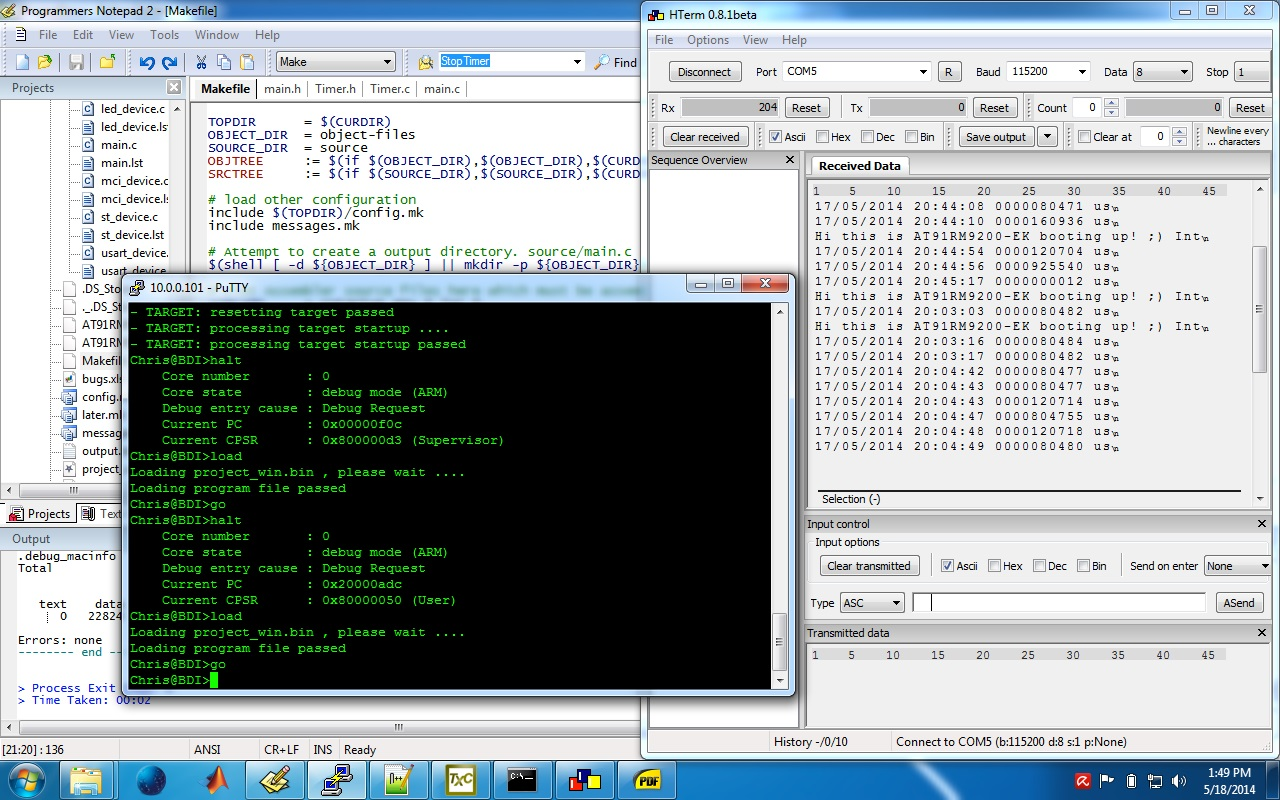
\includegraphics[height=4em]{images/IDE.jpg}};
\node [block, right of=pc, xshift=4cm] 		(BDI) {BDI2000\\ 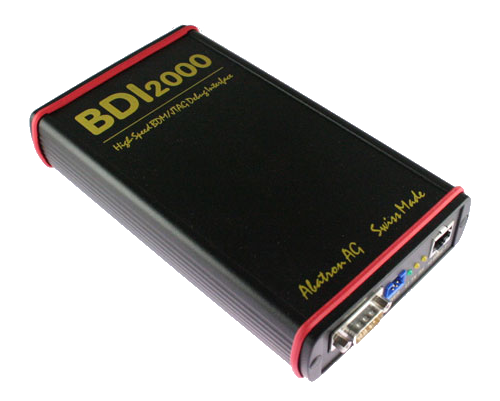
\includegraphics[height=4em]{images/bdi2000.png}};
\node [block, below of=pc] 		(IO) {Input Sensor\\ 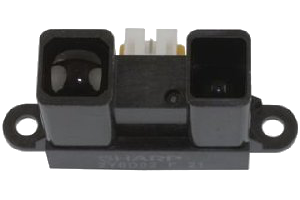
\includegraphics[height=4em]{images/GP2Y0D02YK0F.png}};
\node [block, below of=BDI] 		(AT) {AT91RM9200\\ 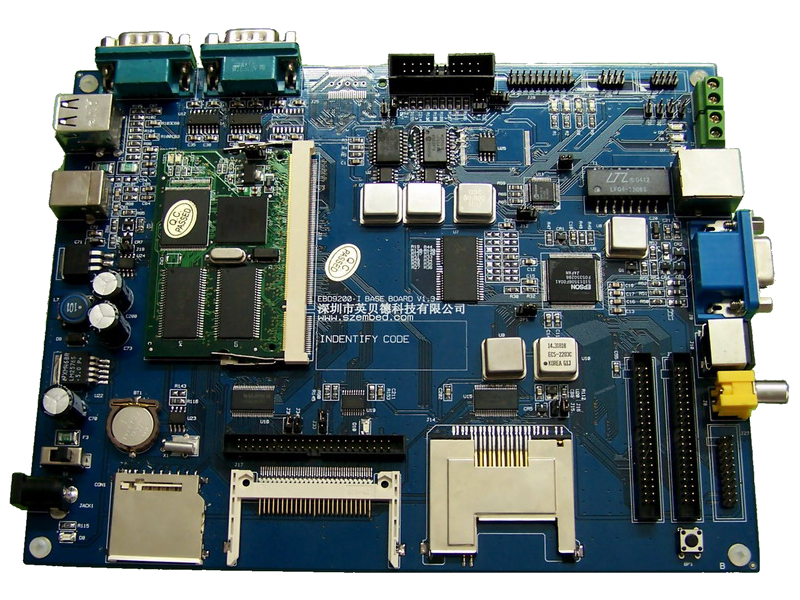
\includegraphics[height=4em]{images/AT91RM9200DB.png}};
%\node [block] 	(um2) {Umrechnung\\ SollTrq $\Rightarrow$ SollPos \\ };
%\node [block,  below of=abstmp] 	(tempmod) {$\Delta$-Temperatur- \\Algorithmus\\  };
%\node [blocksmall,  right of=tempmod, node distance=4cm] 	(multi) {$\times$};
%\node [blocksmall,  right of=multi, node distance=4cm] 	(multi2) {$\times$};
%\node [blocksmall,  above of=multi2] 	(divi) {$\div$};
%\node [blocksmall,  above of=divi] 	(minus) {$-$};
	%
 %
    %% Draw edges
    %\path [line] ([xshift=-2cm,yshift=+0.5cm] abstmp.west)--node [midway, above]{$Act_{Pwr}$}([yshift=+0.5cm] abstmp.west);
%\path [line] ([xshift=-2cm,yshift=-0.5cm] abstmp.west)--node [midway, above]{Tumg}([yshift=-0.5cm] abstmp.west);   
%
%
%\path [line] ([xshift=-2cm,yshift=+0.7cm] tempmod.west)--node [midway, above]{$P_{Eng\_Last}$}([yshift=+0.7cm] tempmod.west);
%\path [line] ([xshift=-2cm ] tempmod.west)--node [midway, above]{$nmot$}( tempmod.west);
%\path [line] ([xshift=-2cm,yshift=-0.7cm] tempmod.west)--node [midway, above]{vfzg}([yshift=-0.7cm] tempmod.west);   
%
%
\draw [dblarrow,<->] ([yshift=0.25cm]pc.east)--node [midway, above]{Ethernet, Telnet}([yshift=0.25cm]BDI.west);  
%\path [line] ([yshift=0.25cm]BDI.west)--node {}([yshift=0.25cm]pc.east);

\draw [dblarrow,<->] (BDI.south)--node [midway, right]{JTAG}(AT.north); 
%\path [line] (AT.north)--node {}(BDI.south); 

\draw [line2] ([yshift=-0.25cm]IO.east)--node [midway, below]{Digital Input}([yshift=-0.25cm]AT.west); 
\draw [dblarrow,<->] ([yshift=-0.25cm]pc.east)--([yshift=-0.25cm,xshift=2cm] pc.east)|-node [near start, above ,rotate=270]{\acs{UART}, RS232}([yshift=0.25cm] AT.west);
%\path [line] ([yshift=0.25cm]AT.west)-|([yshift=-0.25cm,xshift=2cm] pc.east)--([yshift=-0.25cm] pc.east);

%\path [line] ([xshift=-2cm] um2.west)--node [midway, above]{{SollTrq}}(um2.west); 
%\path [line] (abstmp.east)-|node [pos=0.27, above]{$Load_{Fact}$}( multi.north); 
%\path [line] (multi.east)--node [midway, above]{Gew. $\Delta T_{Hydr}$}( multi2.west);  
%\path [line] ([xshift=2cm] multi2.east)--node [midway, above]{$Vol_{Hyd1K}$}(multi2.east);
%\path [line] (multi2.north)--node [midway, above, rotate=90]{$\Delta Vol_{Hydr}$}(divi.south);
%\path [line] ([xshift=-2cm] divi.west)--node [midway, above]{{$Aktor_{Area}$}}(divi.west);   
%\path [line] (divi.north)--node [midway, above, rotate=90]{$Act_{Poscor}$}(minus.south);
%\path [line] (um2.east)--node [midway, above]{$SollPos$}(minus.west);
%\path [line] ( minus.east)--node [midway, above]{$SollPos_{Cor}$}([xshift=2cm] minus.east);
\end{tikzpicture}

		\end{center}
		\caption{System Overview}
		\label{fig:sysov}
\end{figure}


\chapter{Hardware abstraction}
In order to achieve an independent application a \ac{HAL} is introduced in the project. The basic idea is to have a strong decoupling between the different layers in the project. \autoref{fig:Layout} displays the implemented structure. The benefit of this layout is, that with the same \ac{HAL} and therefor the same \ac{API}, a switch to an other target hardware could be realized with no or little changes to the already running application. The so generic designed functionality allows scalability, extendability and hardware independence. Debugging or even the simulation of the application on the host computer is possible.\\
\begin{figure}[H]
		\begin{center}
			% Define block styles
    
\tikzstyle{block} = [rectangle, draw=blue, drop shadow,very thick,top color=white,              % a shading that is white at the top...
    bottom color=blue!20!,%fill=blue!20, 
    text centered, rounded corners, minimum height=1cm,node distance=1.3cm,]
 
 \tikzstyle{blockred} =  [rectangle, draw=red, drop shadow,very thick,top color=white,              % a shading that is white at the top...
    bottom color=red!20!,%fill=blue!20, 
    text centered, rounded corners, minimum height=1cm,node distance=1.3cm,]

\tikzstyle{blockgreen} = [rectangle, draw=green, drop shadow,very thick,top color=white,              % a shading that is white at the top...
    bottom color=green!20!,%fill=blue!20,
		text centered, rounded corners, minimum height=1cm,node distance=1.3cm,]
		
\tikzstyle{blocktrans} = [rectangle, draw=white,top color=white,              % a shading that is white at the top...
    bottom color=white,%fill=blue!20,
		text centered, rounded corners, minimum height=1cm,node distance=1.3cm,]

 

\tikzstyle{line} = [draw,line width=1.0pt, -latex']
    
\begin{tikzpicture}[node distance = 0cm, auto]
    % Place nodes

		\node [blockgreen,minimum width=\textwidth] 	(APPL) {Application};

		

		\node [block,minimum width=0.653333333333\textwidth, below of=APPL, xshift=-0.17333333\textwidth] 	(HAL) {Hardware Abstraction Layer};


		\node [blockred,minimum width=0.306666666\textwidth, below of=APPL, xshift=0.346666666\textwidth] 	(ILMS) {Interrupt Measurement};

		
		\begin{scope}[minimum width=0.1333333\textwidth]
		\node [block, below of=HAL, xshift=-0.26\textwidth] 	(LED) {LED};
		\node [block, below of=HAL, xshift=-0.086666666\textwidth] 	(UART) {UART};
		%\node [block, below of=HAL, xshift=0.086666666\textwidth] 	(USB) {USB};
		\node [blocktrans, below of=HAL, xshift=0.086666666\textwidth] 	(ASO) {$\bullet\bullet\bullet$};
		\node [block, below of=HAL, xshift=0.26\textwidth] 	(IO) {I/O};
		\node [blockred, below of=HAL, xshift=0.4333333333333\textwidth] 	(TI) {Timer};
		\node [blockred, below of=HAL, xshift=0.60666666666\textwidth] 	(COV) {Conversion};
		\end{scope}
		
%%		\node [blockgreen, below of=COV,text centered] 	(T) {TEST};
		

%\node [block] 	(LED) {LED};
%\node [block, right of=LED] 	(UART) {UART};
%\node [block, right of=UART] 	(USB) {USB};
%\node [block, right of=USB] 	(IO) {I/O};
%\node [block, right of=IO] 	(TI) {Timer};
%\node [block, right of=TI] 	(COV) {Conversion};
%\node [block, above of=LED] 	(HAL) [fit=(LED)(UART)(USB)(IO)]{Hardware Abstraction Layer};
%\node [block, above of=TI] 	(ILMS) [fit=(TI)(COV)]{ILMS};
%\node [blockgreen, above of=HAL] 	(APPL) [fit=(HAL)(ILMS)]{Application};




\end{tikzpicture}

		\end{center}
		\caption{Projekt \acs{HAL} layout}
		\label{fig:Layout}
\end{figure}
The layering in this project focus most on an abstraction of the hardware interfaces. There are for example different LED-commands allows the higher layers to turn on, off or toggle the states of one or more LED's with out knowing the hardware address or the circuit design. Such high level commands are also available for the \ac{UART} interface. Serving simple send and receive functions for the application or other function. A similar hardware abstraction is also achieved for the I/O's. The application doesn't to take care of configuring, masking or filtering the I/O. For example digital input function delivers only true or false as the input state. 
This \ac{HAL} serves strict information hiding.This means in terms of the application that it has no direct hardware access. This is only realizable for limited functionality. Some real time critical services needs to accomplish fast reaction times and reach hard deadlines, via a direct hardware access. These services can not afford to go through the complete stack or layers. The in this project work realized \ac{ILMS} is an example for such a service. Due to short latency to serve and measure an interrupt, to wait until a timer is available is not possible for this kind of service. Therefor like shown in \autoref{fig:Layout}, one timer unit belong to the service as well as conversion function which is needed to convert the results into a human readable format.\\

\section{LED}
\label{sec:LED}
The development hosts 3 different LEDs. The LEDs are controllable via different bits inside the memory mapped IO. \autoref{LEDDef} is the pin definition according to the circuit schematic (\autoref{fig:LEDsche}). This allows for the LED-functions to use symbolic names and also be concatenated inside the function calls (E.g. "resetLed(GREEN | RED | YELLOW );").\\

\begin{lstlisting}[language=C, caption={Color definition for the LED-functions}, label={LEDDef}]
#define GREEN  ((unsigned char) (1<<0))
#define YELLOW ((unsigned char) (1<<1))
#define RED    ((unsigned char) (1<<2))
\end{lstlisting}

The LED itself are low active. This means to be turned on a low voltage needs to be supplied at the corresponding output pin \cite{AT91LED}.\\
The existed LED driver was changed and reworked in a way that the state of the LED is controlled via the output voltage. The old output enable based concept had the flaw that some unknown high frequency dimed the YELLOW-Led. The output signal is now also for extendability available at the output pins.
\begin{lstlisting}[language=C, caption={Configure the LED-Pins as output}, label={LED-Init}]
void Led_init()
{	
  //Enable Register!                                                    
	AT91C_BASE_PIOB->PIO_PER  = AT91C_PIO_PB0|AT91C_PIO_PB1|AT91C_PIO_PB2;
  //Enable output!
	AT91C_BASE_PIOB->PIO_OER  = AT91C_PIO_PB0|AT91C_PIO_PB1|AT91C_PIO_PB2; 
	//Assign PB.0-2 to GND
	AT91C_BASE_PIOB->PIO_CODR = AT91C_PIO_PB0|AT91C_PIO_PB1|AT91C_PIO_PB2; 
}
\end{lstlisting}
\autoref{LED-Init} displays the Led\_init()-function. The \acs{PIO}\_PER (\acs{PIO} Enable Register) is set with the pins of the LED (PortB0-2). The output at the LED-pins is enabled via the \acs{PIO}\_OER (\acs{PIO} Output Enable Register). To finish the initialization all LEDs are activated through a set in the \acs{PIO}\_CODR (\acs{PIO} Clear Output Data Register). This is done to achieve a definite output state after initialization. The complex IO-register features via the clear and set-registers an adjustment of output pins without a read command of the current output state, followed by a dis- or conjunction and a final store command. This reduces needed processor clock cycles and registers for such small IO-operation to an (if possible) atomic instruction.\\
\autoref{tab:LEDcomands} lists the available LED-functions:

\begin{table}[H]
\begin{tabular}{llll} %\hline
\textbf{Function Call}	 &\textbf{Parameters}  &\textbf{Return} &\textbf{Description} \\
\hline
\hline
Led\_init									&None 	&None & Initialize the LED-pins, turns on all LEDs\\
toggleLed			&Symbolic Name 	&None & Toggles the output of the specified LED(s)\\
setLed					&Symbolic Name 	&None & Turns on the specified LED(s)\\
resetLed			&Symbolic Name 	&None & Turns off the specified LED(s)\\
getLed	&Symbolic Name 	&State & Returns LED(s) state\\ 
\end{tabular}
\caption{LED-functions}
\label{tab:LEDcomands}
\end{table}

\autoref{fig:LEDsche} is an extract of the development board schematic. The LEDs are supplied with 3.3V and a LED independent series resistor of $220\Omega$. The assignment to the corresponding hardware pis is also indicated.\\ 

\begin{figure}[H]
\begin{center}
	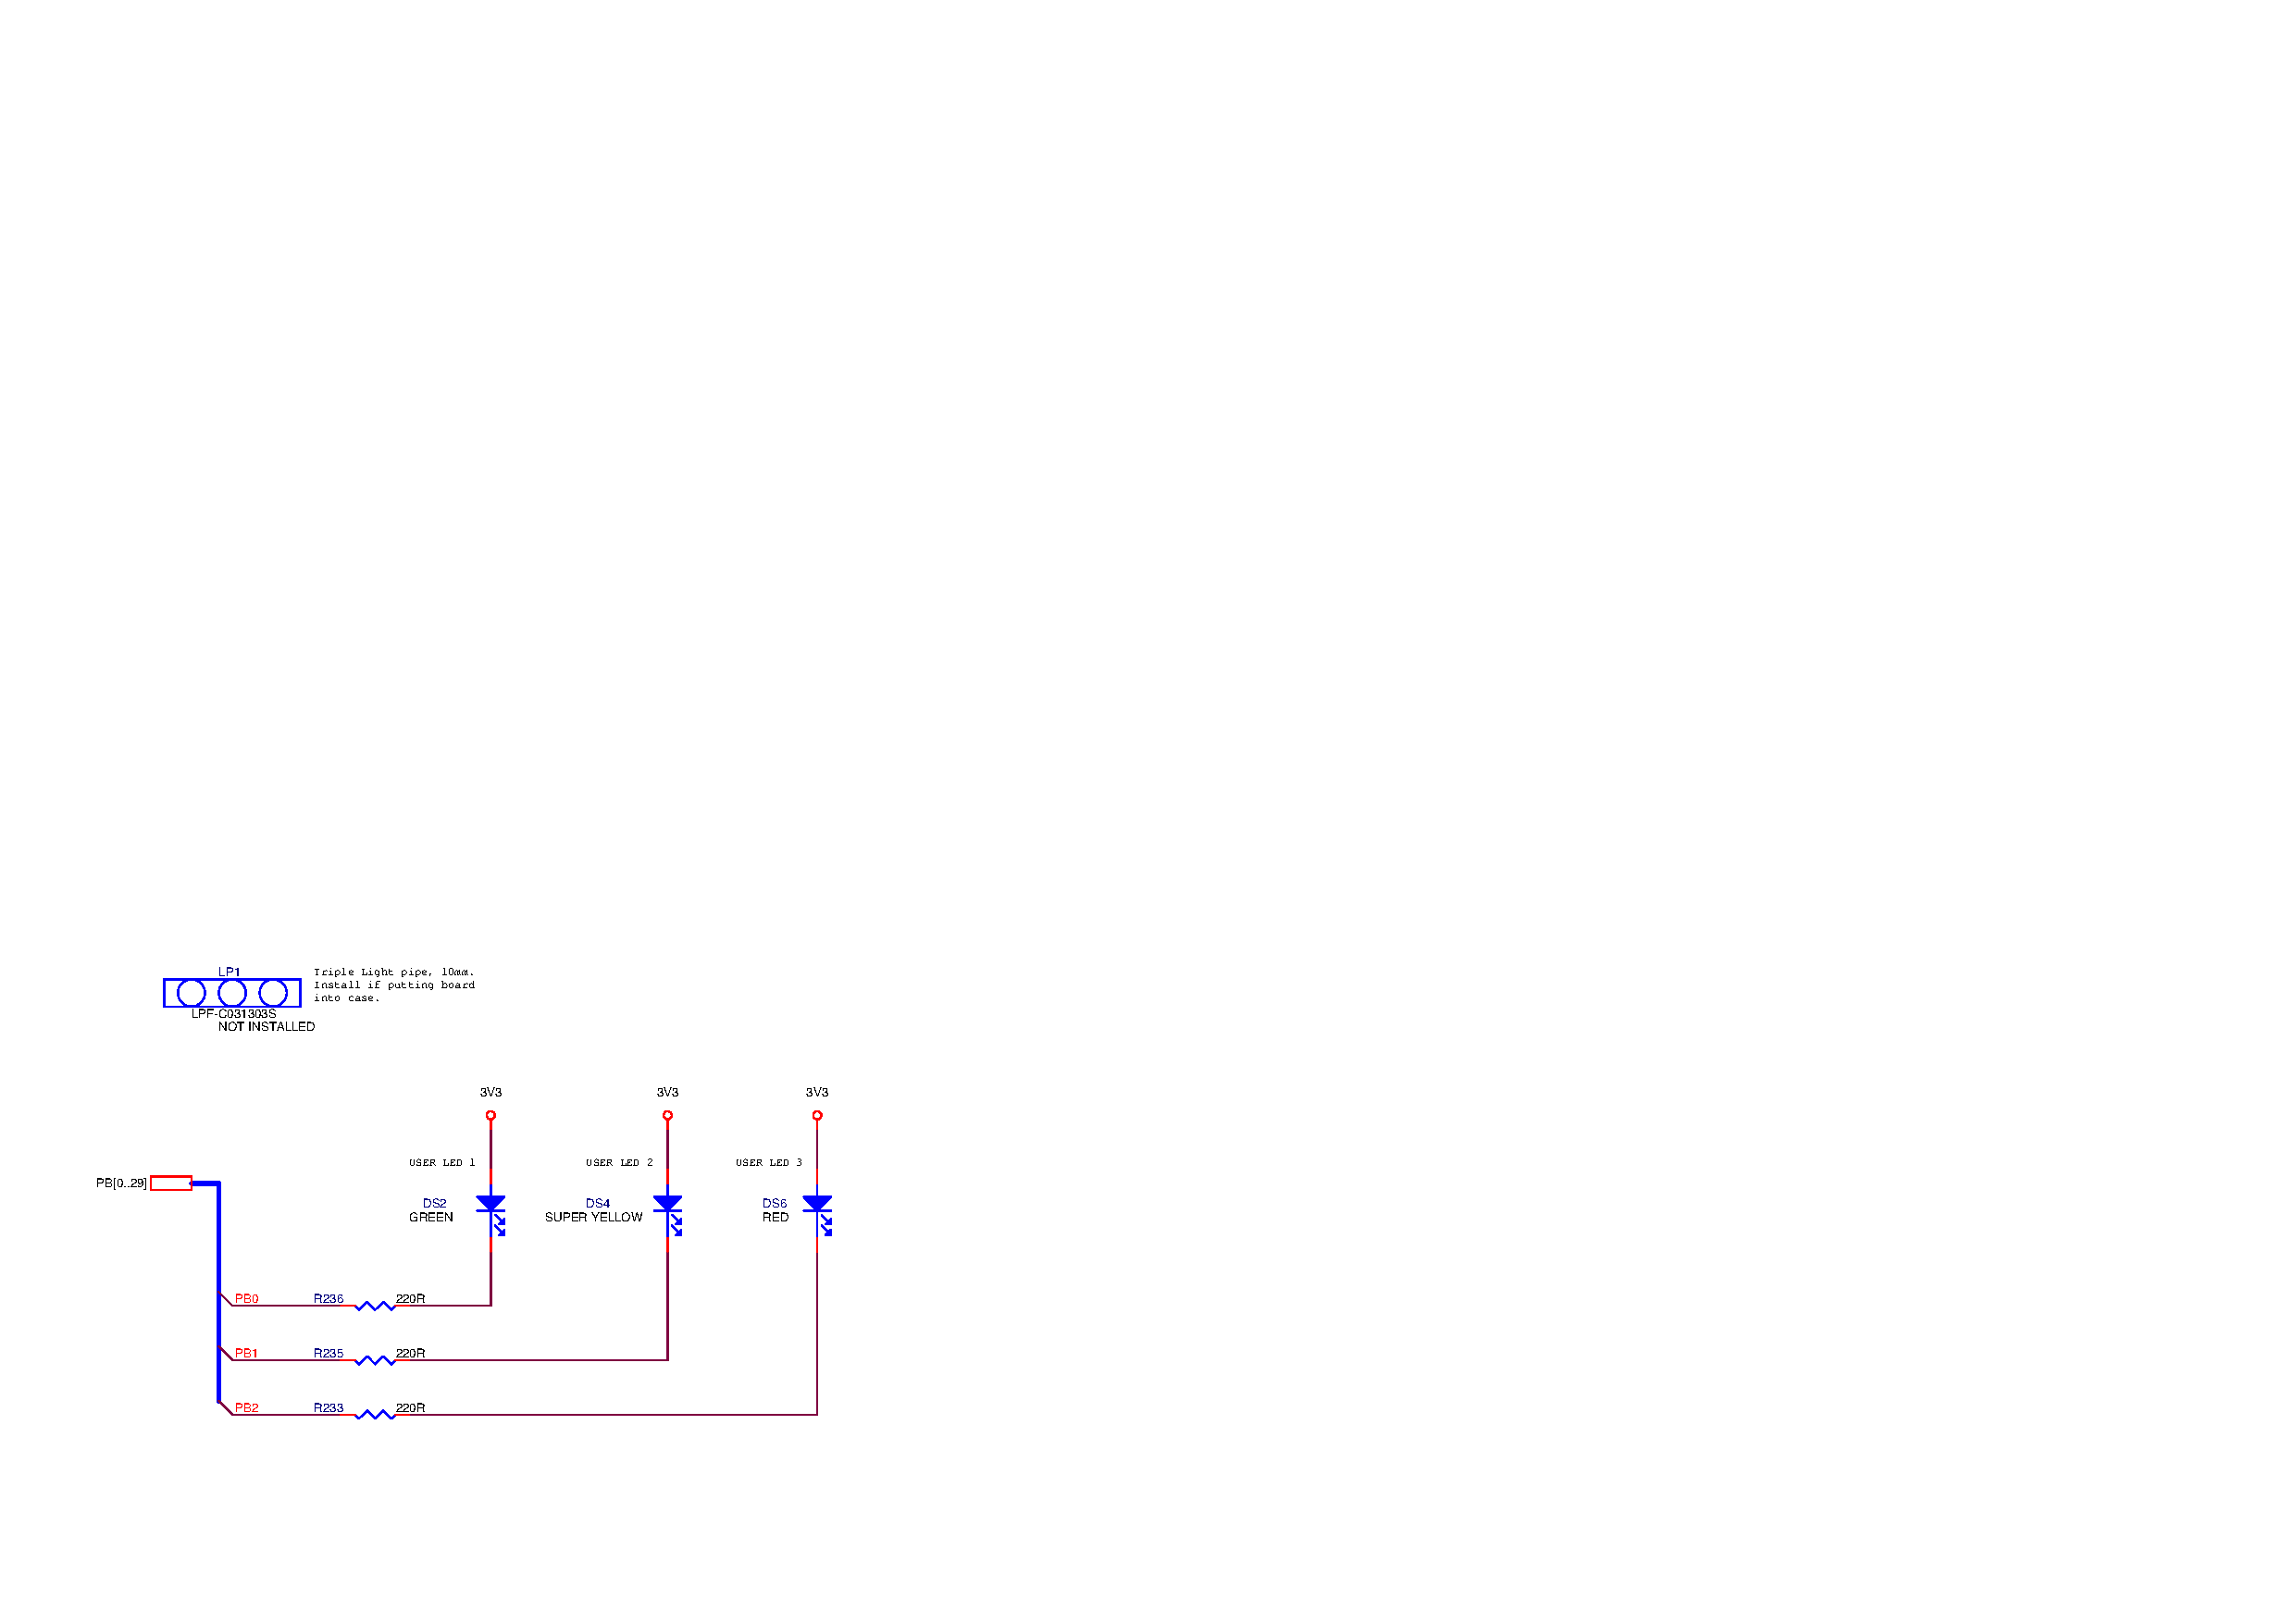
\includegraphics[width=0.8\textwidth]{images/LedScematic.pdf}
		\caption[LED Schematic AT91RM9200\_EK] {LED Schematic AT91RM9200\_EK \cite{AT91LED}}
	\label{fig:LEDsche}
\end{center}
\end{figure}




%\section{IO's}


\section{\acs{UART}}
\label{sec:RS232}
The \acf{UART} is a widely used interface in embedded systems. It's simple to configure and features flexible data rates as well as wiring length. Also different physical mediums can be used. The protocol transmit short messages containing only several bits. How ever there is is no clock synchronization, therefor the specified clock frequency has to have such a precision, to stay with in all bit timings of a transmitted frame. The interface features handshaking mechanism, but a simple serial bidirectional communication can be achieved with only 3 wires.\\
The used protocol in this project is the RS232. The features are transmission between 5 and maximally 9 bits of data. The frame itself begins with a start bit followed by the data. A one bit parity field allows error detection of all odd number of bit errors. The frame is ended 1,1.5 or 2 bits known as stop bit.\\
The RS232 specifies a negative logic for the computer to computer connection. The voltage levels need to be converted via a level converter into a positive logic with the processor voltage levels.\\
The \autoref{tab:RS232Set} shows the communication settings of the user as well as the debug interface. The handshaking mechanism is not used.\\

\begin{table}[H]
\begin{tabularx}{\textwidth}{llllll} %\hline
\textbf{Baud Rate}	 &\textbf{Data bits}  &\textbf{Parity} &\textbf{Stop Bit}&\textbf{Handshake}& \textbf{Type} \\
\hline
\hline
115200&8	& None & 1& Not used & Bidirectional\\
\end{tabularx}
\caption{User RS232 settings (8-N-1)}
\label{tab:RS232Set}
\end{table}

There are different methods for sending and receiving the data. The controller features a fully in hardware realized \ac{UART} transceiver. Therefor the received data is available for the application in a message buffer. For transmission a register used as a buffer to send out the data as soon as the there is no other data in transmission. The following enumeration explains 4 possible ways:

\begin{itemize}
	\item \textbf{Blocking:}\\
In case of receiving the application looks with a blocking function call if there is a new message in the buffer. If not it just loops the receiving status bit until there is new message available. This is called blocking, because the processor is fully occupied with the task of waiting till the status bit indicates successful received data.
For sending the core is blocked while waiting, before the data is stored in the transmission buffer. This is not suitable for an application, because if there is no data incoming or the transmission buffer is full, this will lead to a dead lock.\\
	\item \textbf{Polling:}\\
	An other possibility is the polling approach. This differs between the blocking in the way of testing if transmission or new data is present. The application can check time or event based and if the communication interface is not applicable, continue with its other tasks. The polling frequency needs to be higher as the baud rate of the \ac{UART}. How ever if the application load increases the the polling frequency (if not interrupt handled) decreases. This may lead to data loss on the receiving site or an decrease in data throughput on the sending side.\\
	\item \textbf{Interrupt:}\\
Interrupt handling for the receive case ensures no loss in data an a fast processing. As soon as valid data is available the generated interrupt executes the corresponding \ac{ISR}. The data is processed there. The core is only interrupted if new data is waiting for processing. In the case of no communication the processor has the full processing power to handle other tasks. To send data also an interrupt is generated when transmission is possible.
When there is long communication ongoing, the processors load is increased. The core has to serve the \ac{ISR} for every byte. This creates especially with high baud rates a high overhead for entering an exiting the \ac{ISR}.\\
	\item \textbf{\ac{DMA}:}\\
	To reduce the processor load, in the case of heavy communication, the \ac{DMA} controller is used. The feature of the memory access enables in the sending case to only specify a memory pointer and a data length. The peripheral \ac{DMA} controller then starts with the transmission till all data is transmitted. The processor therefor has to be interrupted only once. For receiving the \ac{DMA} can be configured in a way, such that all incomming data is stored into a specific location in the memory. An interrupt then could be triggered if the buffer is full or all data is available.\\
This method is used to transmit the result of the \ac{ILMS}. The AT91RM9200 features also a transmit next register to start a transmission right after the first one has finished.\cite{AT91DMA}\\
\end{itemize}


%################################################################################################

\newpage
%\subsection{USB}
\section{Digital Input}
For demo purpose (\autoref{DemoInt}) the duration of the high pulse of an digital input is measured. The distance measuring sensor unit (\autoref{UVsens}) is connected to the development board.\\
The microcontroller includes with the \acf{PIO} a fully programmable input/output controller. Other as in \autoref{sec:LED} the pin has to be configured as an input.\\
The controller provides features like, programmable pull up resistors, input glitch filter as well as an input change interrupt. Because of the connected input sensor neither input filtering nor a pull up resistor (connected on the sensor side) is necessary.\\ 
\autoref{IOCFG} gives an overview how the hardware input is configured. The InitDemoInterrupt function call (line 2) displays all function parameter by there mnemonic. At first the \ac{PMC} has to be configured (line 5). A special feature of the processor is \ac{PMC} peripheral clock configuration. The activation of the corresponding pin enables the update of the pin status with the master clock frequency. If not enabled the input pin stores the last level when a the clock was enabled. Best practice is to disable the input clock for not used inputs, after they have executed their last operation.\cite{AT91PMC}\\
To be able to read input signals the pin has to be configured as input. This is done with the AT91F\_PIO\_CfgInput-function. The function performs two operations. The output of this pin is deactivated and the pin is enabled.\\
Line 7 configures the \ac{AIC} (see \autoref{sec:AIC} for details) with the interrupt priority, the interrupt type and also the address where the \ac{ISR} is located. Line 8 and 10 enables the interrupt. First in the \ac{PIO}-controller and then in the \ac{AIC}.\\
Reading the \ac{PIO}\_ISR (Interrupt Status Register) is necessary because the hardware only features an change interrupt. So when ever the interrupt occurs before the programming of the \ac{AIC} or was not served the last time it needs to be cleared. This is done via reading the status register causing a clear of all pending \ac{PIO} interrupts. When then the next \ac{PIO} interrupts occurs the \ac{AIC} can serve the change and run the corresponding \ac{ISR}. An pending not served interrupt would be equivalent to a constant high level and would be never processed because of no change in the status register. Also any new interrupt would not affect this, because the status would just keep its value.\cite{AT91PIO}\\




\begin{lstlisting}[language=C, caption={Demo interrupt at PB15 configured as rising}, label={IOCFG}]
// Function call with parameters
	InitDemoInterrupt(AT91C_BASE_PIOB,AT91C_ID_PIOB, MY_INT_PIN, AT91C_AIC_PRIOR_LOWEST, AT91C_AIC_SRCTYPE_EXT_POSITIVE_EDGE);

void InitDemoInterrupt(AT91PS_PIO PIOptr, unsigned int ParallelID, unsigned int MyIOpin, unsigned int priority, unsigned int intType){
			AT91F_PMC_EnablePeriphClock (AT91C_BASE_PMC, ((unsigned int) 1 << ParallelID));
			AT91F_PIO_CfgInput (PIOptr, MyIOpin); 
			AT91F_AIC_ConfigureIt(AT91C_BASE_AIC,ParallelID,priority,intType,Measured_Interrupt_Lowlevel);
			AT91F_PIO_InterruptEnable (PIOptr, MyIOpin);
			{volatile unsigned int dummy; dummy = PIOptr -> PIO_ISR;}
			AT91F_AIC_EnableIt (AT91C_BASE_AIC, ParallelID); }
\end{lstlisting}

\subsection{Sharp sensor}
\label{UVsens}
The Sharp sensor GP2Y0D02YK0F (figure \ref{fig:sharpPic} is a distance measuring sensor with a range up to 80 cm. It provides an digital output high if an object is with in the range of the sensor. The measuring principle is based on an infrared emitting diode. Figure \ref{fig:sharpSchema} illustrates the different blocks of the sensor. The emitted light is processed in a position sensitive detector (PSD) and the signal processing circuit provides the digital output. To avoid toggling the sensor has a hysteresis of about 10 cm. Also because of the sensor design, measurements closer than approximately 4 cm are not possible. In conclusion with the in accuracy of the sensor the detecting range is between 4 cm and 80 $\pm$ 10 cm. The sensor needs a power supply of around 5V with maximally 50 mA of current. The output stage is a so called open collector output and needs an external pull up resistor around 12 k$\Omega$. The sensor is wired according to the recommended values. The power supply is connected to a \ac{USB} port of the development board. The output is connected to PB15 which is located at pin C42 of the expansion slot.\cite{sharp}\\

\begin{figure}[H]
\begin{center}
		  \subfigure[Sharp GP2Y0D02YK0F]{
    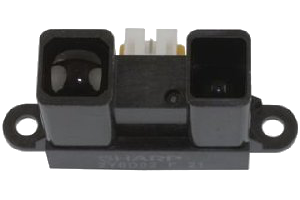
\includegraphics[width=0.42\textwidth]{images/GP2Y0D02YK0F.png}
		\label{fig:sharpPic}}
			\hspace{0.8 cm}
    \subfigure[Schematic of the sensor supply]{
   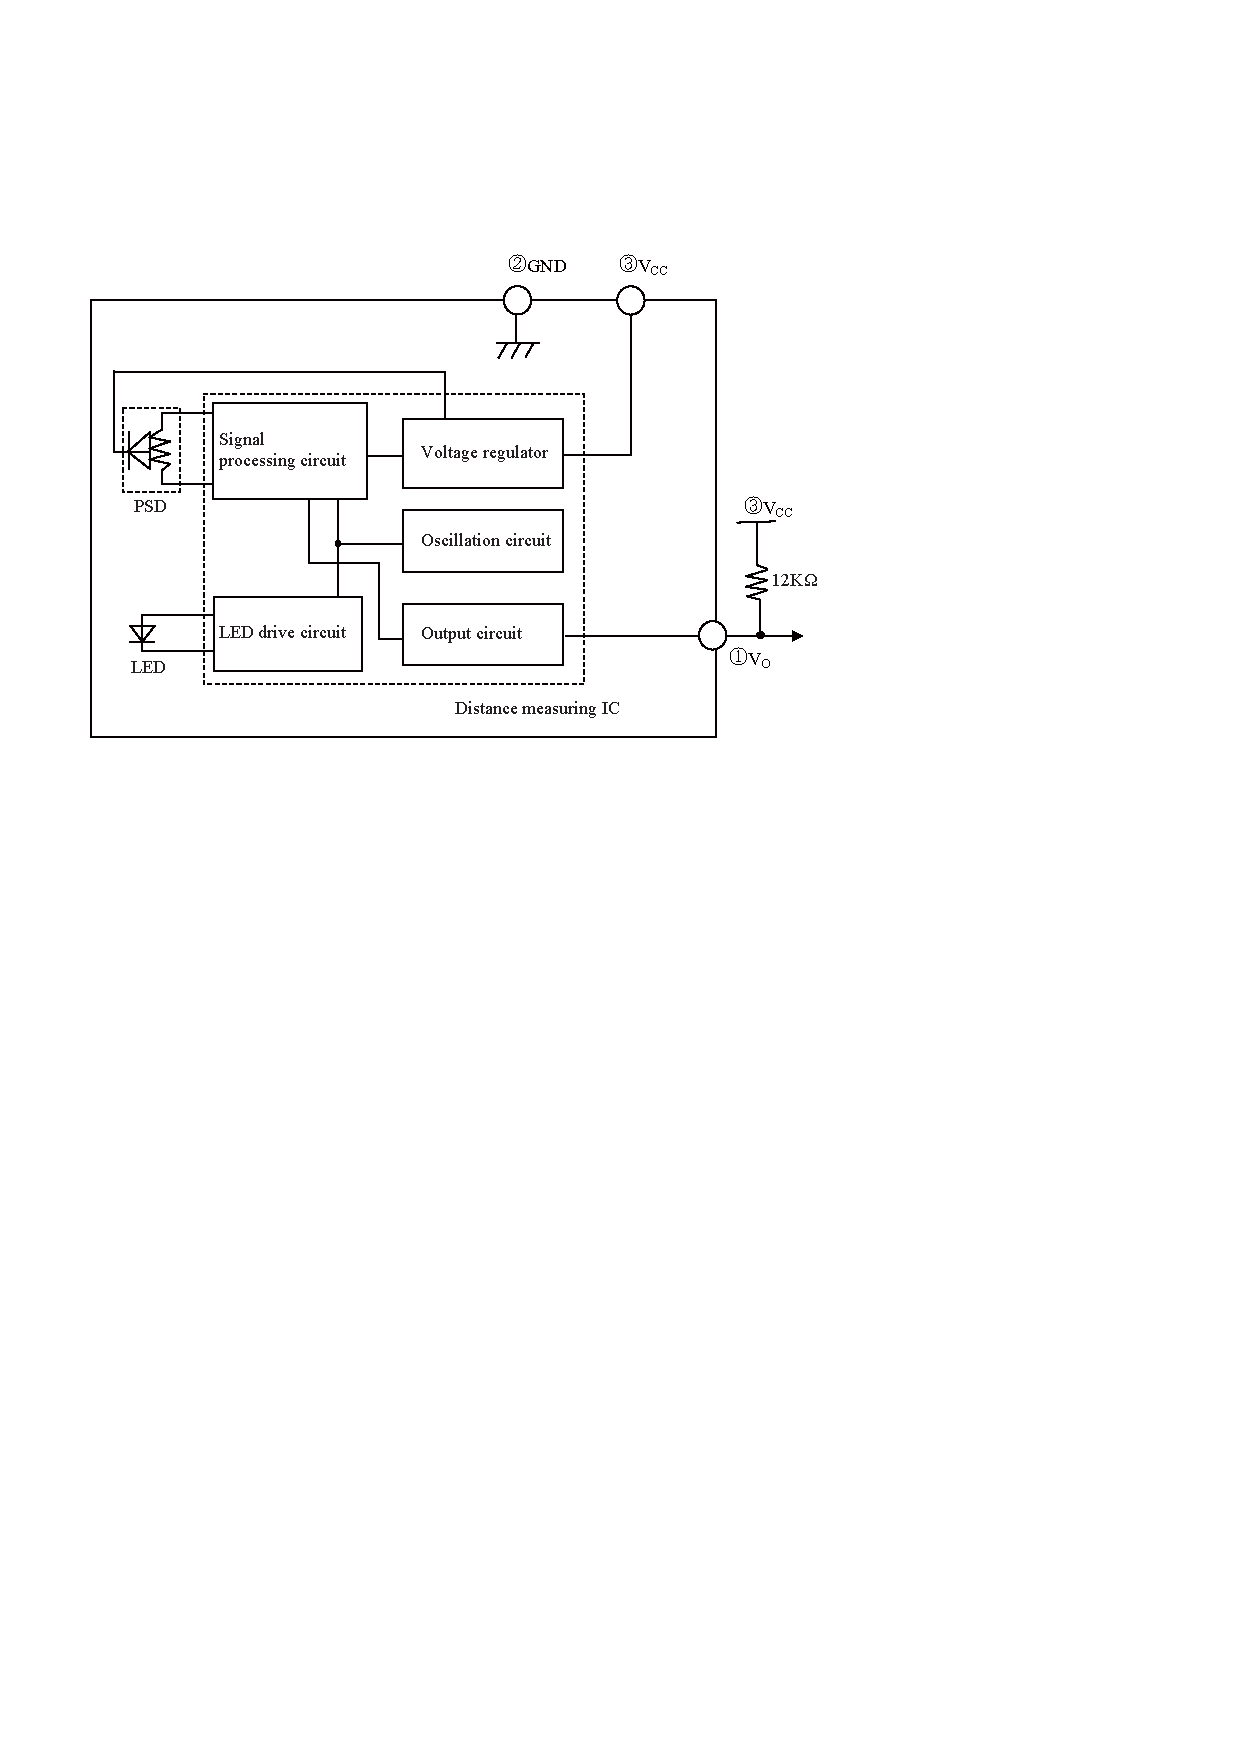
\includegraphics[width=0.42\textwidth]{images/SharpSchematics.pdf}
		\label{fig:sharpSchema}}
		\caption[Sharp GP2Y0D02YK0F Distance Measuring Sensor Unit]{Sharp GP2Y0D02YK0F Distance Measuring Sensor Unit \cite{sharp}}
		\label{fig:sharp}
		\end{center}
\end{figure}

\newpage
The sensor provides a stable output signal of around 40 ms. \autoref{fig:Sharptiming} displays the timing behavior of the sensor. The sensor update frequency is according to the timing limited by around 25 Hz. This is beneficial for the input of the microcontroller, because there is no need to filter this preprocessed, stable input signal. Line 4 in the \autoref{tab:Demointres} is a measurement of the shortest possible sensor high level duration. It is around 40.232 ms and with that in the range of the specified 38.3 $\pm$ 9.6 ms. Due to this fact all demo measurements of this table, are multiple of this duration. For example line 6 is a duration of 1167.025 ms and is approximately 29 times the minimum duration.\\

\begin{figure}[H]
\begin{center}
	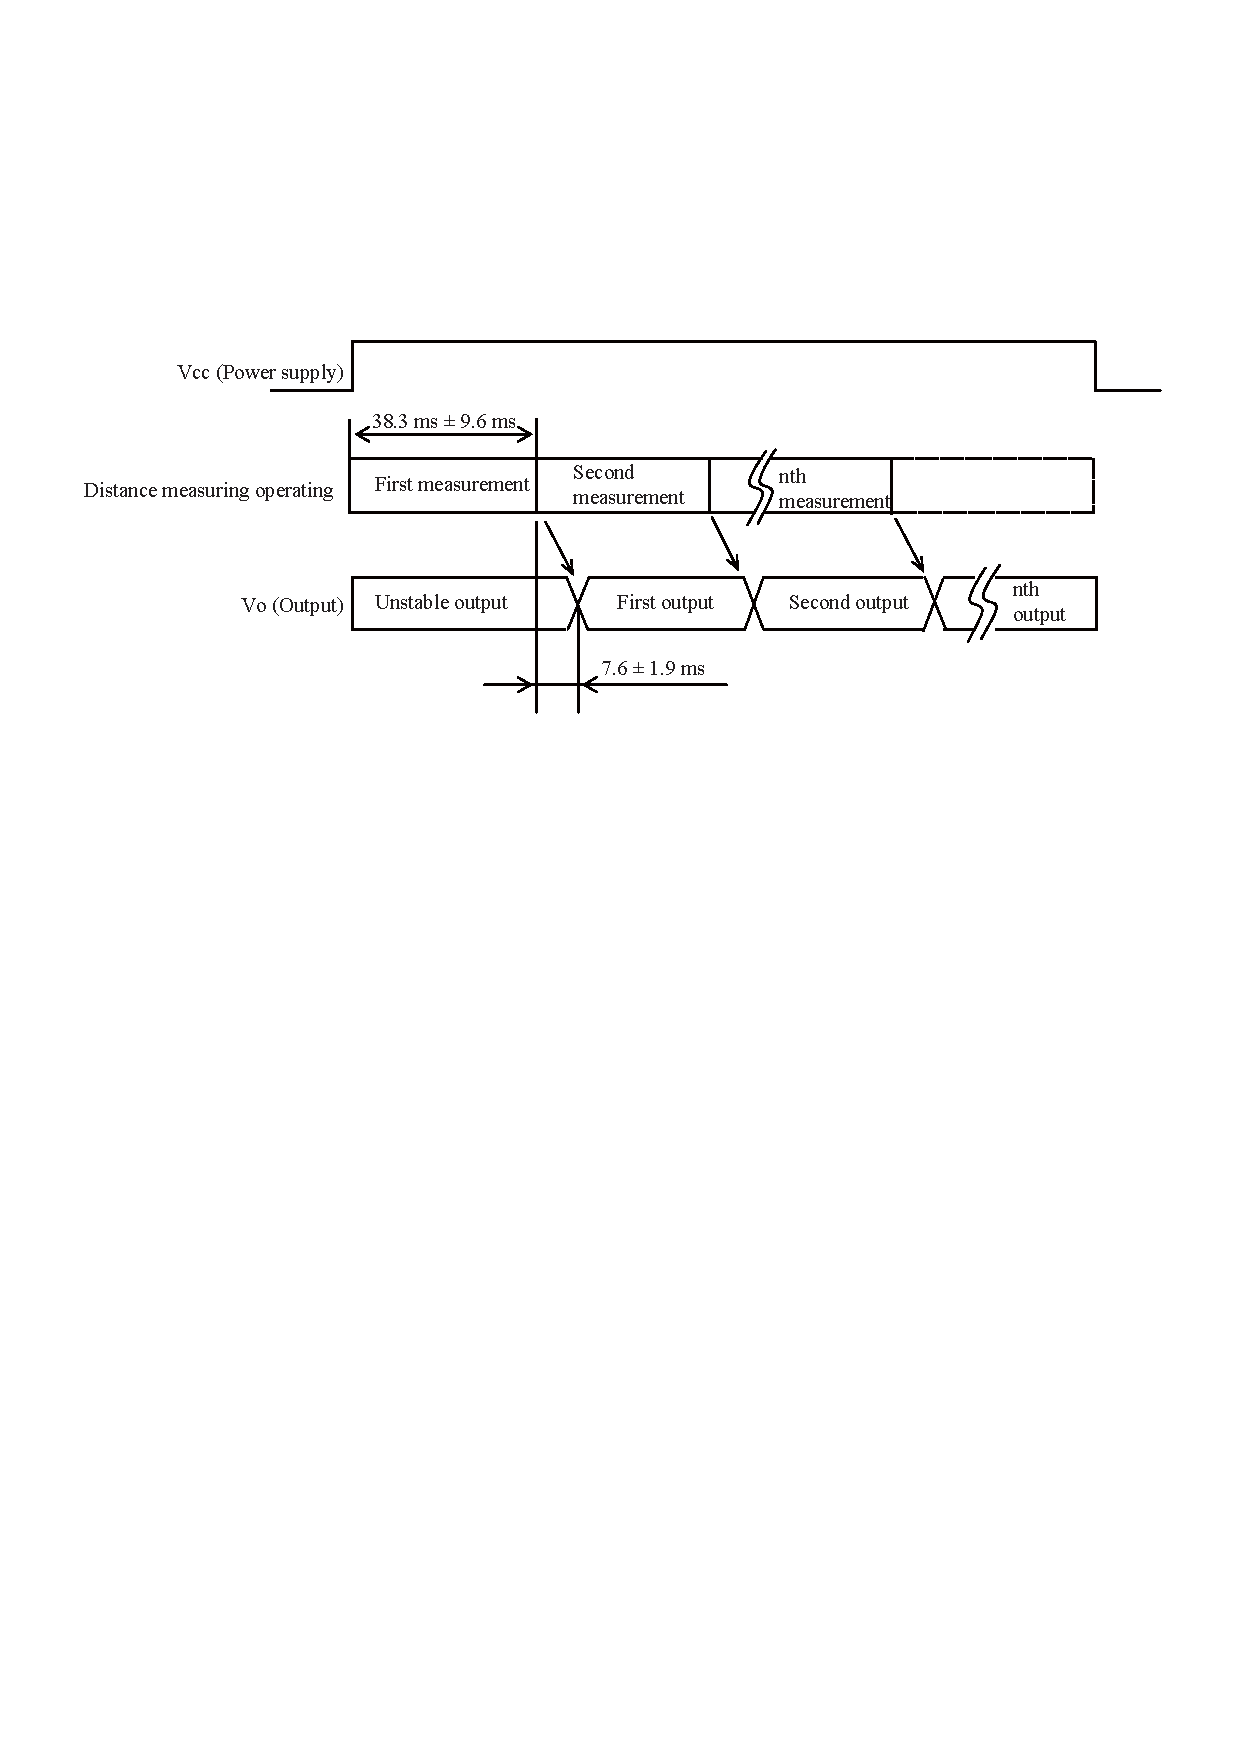
\includegraphics[width=0.8\textwidth]{images/SharpTiming.pdf}
		\caption[Sharp timing chart] {Sharp timing chart\cite{sharp}}
	\label{fig:Sharptiming}
\end{center}
\end{figure}



\section{\acs{RTC}}
\label{RTCchapter} 
The controller features a hardware \acf{RTC}. It's used inside this project to supply the date and time stamp when an measured interrupt has occurred. The \ac{RTC} has low power consumption and 200 year calendar. Also different interrupts can be triggered via programmable interrupts. The device uses the SLCK (32768 Hz) and divides this clock by 32768 to get a high precision 1 Hz clock. Time and date counting is done in hardware. The values are present in the \acf{BCD} format. This means each decimal is represented via 4 bits. Lower 4 bits encodes the unit and the upper 4 bits the tens.\cite{AT91RTC}\\
\autoref{RTCInit} lists the different commands to setup and initialize the \acs{RTC}. Line 3 checks and waits till the SEC flag is set. This is done because the user has to wait at least one second after the last update (only necessary for high frequent updating). Next the flags for updating time and date are set in the \acs{RTC} Control Register. The user also has to wait here, until the acknowledge is set in the \acs{RTC} Status Register. Line 6 selects the 24 hour mode. The next commands fills the date and time structures with the user defined settings. These two 32 bit values are stored in line 18 \& 19 in the \ac{RTC} time and date registers. These values are checked if they contain the right format and possible values. Otherwise the values are silently discarded. The clear in the next line disables the update request for time and date. The \ac{RTC} starts running again. And SEC flag is cleared with the next command to wait at least one second before re updating the time.\cite{AT91RTC}\\

\begin{lstlisting}[language=C, caption={Minimal \acs{RTC} initialization}, label={RTCInit}]
void Rtc_init(void) 
{	
	while (!(AT91C_BASE_RTC->RTC_SR & AT91C_RTC_SECEV) ); 
	AT91C_BASE_RTC->RTC_CR      = (AT91C_RTC_UPDTIM | AT91C_RTC_UPDCAL); 
	while (!(AT91C_BASE_RTC->RTC_SR & AT91C_RTC_ACKUPD) ); 
	AT91C_BASE_RTC->RTC_MR 		  = 0;         	
	rtc_time.time_bits.second 	= 0x00; 
	rtc_time.time_bits.minute 	= 0x35; 
	rtc_time.time_bits.hour 	  = 0x16; 
	rtc_time.time_bits.merid 	  = 0x00;
	
	rtc_cal.cal_bits.century 	  = 0x20; 
	rtc_cal.cal_bits.year 		  = 0x14; 
	rtc_cal.cal_bits.month 		  = 0x06; 
	rtc_cal.cal_bits.day 		    = 0x06; 
	rtc_cal.cal_bits.date 		  = 0x02;
	
	AT91C_BASE_RTC->RTC_TIMR    = (uint32)rtc_time.time_data;	
	AT91C_BASE_RTC->RTC_CALR    = (uint32)rtc_cal.cal_data;
	
	AT91C_BASE_RTC->RTC_CR 			= 0; 			
	AT91C_BASE_RTC->RTC_SCCR 		= AT91C_RTC_SECEV; 
}
\end{lstlisting}




%############################################################################################################

\chapter{Interrupt Latency Measurement Service}
\label{sec:ILMS}

The \acf{ILMS} provides a service to measure the computation time of interrupts. This could be used to check for real time capabilities of a measured task or record the worst case execution time in a test scenario. This is done by observing and recording any duration the interrupt needed with different load scenarios. Also long run times in terms of weeks or months may elongate interrupts and increase the used stack. This latency measurement is calculated with the \ac{ILMS} and transmitted over \ac{UART} (\autoref{tab:FC}) to a running and receiving database. A timestamp specifies the point in time when the execution of the interrupt started. For better readability this frame is transmitted as ASCII so also a standalone logging via a serial recorder is possible. The service is implemented in a way to use as less as possible resources of the processor and if possible compensate the measured result (see \ref{correction} for details). In order to archive for the application or programmer an easy way to specify a task to be measured, only the \ac{ISR} needs to be set to the "Measured\_Interrupt\_Lowlevel". The programmers \ac{ISR} then is automatically available as "Measured\_Interrupt\_Highlevel".\\
The main idea behind this is to start a timer, as soon as the low level routine is called through the \ac{AIC}. At this point also the time stamp is saved. After this the high level routine is loaded and executed. After the task is completed the timer is stopped and based on the timer and master clock frequency a duration of the task is calculated. The result is converted in to ASCII and transmitted via the \ac{DMA} through the \ac{UART} interface. This method allows an on chip measurement of the latency as well as serving nested interrupts.\\

\section{\ac{AIC}}
\label{sec:AIC}
The microcontroller includes also an \acf{AIC}. This allows the user to assign a priority form 0 to 7 for each interrupt source. That permits that higher prioritized interrupts to be executed even if a lower prioritized \ac{ISR} is executed at that time (interrupt nesting). The controller features different interrupt types for internal and external interrupts. Besides the priority, \acf{FIQ} and regular \acf{IRQ} can be processed. The \ac{FIQ} is always connected to the interrupt source 0. Banked registers enables a short context switch (\autoref{atcore} and \autoref{tab:regs}). Source 1 is reserved for system peripherals and source 2 to 31 for embedded peripheral or external interrupts. In this project the interrupt sources are, 3 for the digital input and 17 for the timer. The \ac{AIC} is not affected by the \ac{PMC} and no interrupt clock needs to be configured. Also vectoring provides an optimized way for branch and execution.\cite{AT91AIC}\\ % (\autoref{TimerCfg})

\section{\acs{ILMS} initialization}
The \ac{ILMS} provides 3 core functions. An extract of the "InterruptMeasurmentService.h" in \autoref{IMSH} displays these with their parameters. Before using the \ac{ILMS} the service needs to be initialized.\\
\begin{lstlisting}[language=C, caption={InterruptMeasurmentService.h functions}, label={IMSH}]
//InterruptMeasurmentService.h
void Init_Latency_Measurement	(unsigned char TimerClockBase,unsigned char TimerInterruptCompensation);
void Start_Latency_Measurement(void);
void Stop_Latency_Measurement	(void);
\end{lstlisting}
The init-command initialize the timer with the specified clock frequency. The mnemonics and resulting timer frequencies are specified in \autoref{tab:defines}. Also the last column indicates the maximum measurement duration without triggering an timer overflow (16 bit counter) at master clock speed of 60 MHz. Both input parameters are stored in the \ac{ILMS} environment to be used later on. Also a reconfiguration during run time would be possible. Similar to the I/O-configuration (\autoref{IOCFG}) the timer interrupt is configured and enabled. Compared to the lowest priority for the demo interrupt, the timer overflow requires the highest interrupt. This permits the overflow \ac{ISR} to be executed even if nested interrupts are being processed at this time (\autoref{timerovfl}.\\

\begin{table}[H]
\begin{tabular}{lllS[table-format=4.2]} %\hline
\textbf{Mnemonic}  &\textbf{Value} &\textbf{Description} &\textbf{Max. timer w/o ovfl @60MHz} \\
\hline
\hline
	 TIMER\_CLOCK1 		&0x00   &MCK/2  				& 2184.53 {$\;\mu s$}\\
	 TIMER\_CLOCK2 		&0x01		&MCK/8					&8738.13 {$\;\mu s$}\\
	 TIMER\_CLOCK3 		&0x02		&MCK/32					&34.95 {$\;m s$}\\
	 TIMER\_CLOCK4 		&0x03		&MCK/128				&139.81{$\;m s$}\\
	 TIMER\_CLOCK5 		&0x04		&SLCK (32768Hz)	&2.00 {$\;s\;$}\\
	\hline
	 INT\_COMP\_OFF 		&0x00		&\multicolumn{2}{l}{Correction disabled}\\
	 INT\_COMP\_ON 		&0x01	  &\multicolumn{2}{l}{Correction enabled}\\
\end{tabular}
\caption{mnemonic for timer and interrupt compensation}
\label{tab:defines}
\end{table}
The second function parameter describes if the time compensation for the timer overflow interrupted should be activated or is not required. Subsection \ref{correction} describes the used time approximation. The following enumeration gives examples when to use the compensation and also application where there is no need or a compensation would sophisticate the result:\\
\begin{itemize}
	\item \textbf{INT\_COMP\_OFF:}\\
	Should be used for all sorts of hardware inputs. In general where there are two separate events when the task is started and ended. E.g. input pulse width measurement. Like in the demo interrupt the measurement is started with the rising edge and ended by the falling edge of the digital I/O.\\
	
	\item \textbf{INT\_COMP\_ON:}\\
	For all measured long tasks which fully use the full processor power from start to finish. They could be interrupted by higher prioritized interrupts. How ever a scheduled task can be measured, but depending on the processor load the task may is not elongated through the timer overflow \ac{ISR} and the compensation should be turned off.
\end{itemize}
In general there is no difference for short tasks whether the compensation is active or not. This is only true as long as there is no timer overflow. The clock frequency of the timer (\autoref{tab:defines}) therefor should be a compromise between accuracy and the maximum measurable time span. To just pick the SLCK as the slowest frequency would enable measurements up to 2 s without an timer overflow. However the accuracy per tick is with 30.52 $\mu s$ (master clock 60 MHz) rather low.\\


\section{Interrupt concept}
As mentioned in \autoref{sec:ILMS}, the \ac{ILMS} provides the low level routine with a fixed callback to the application / programmer specified high level \ac{ISR}. \autoref{MILSR} is an extract of the "ISR.S". This part provides low level function. The interrupt entry macro in line 10 switches the processor mode and pushes the user register in the user stack. Also the link register is updated.\\
The "bl" command starts the interrupt latency measurement. The mnemonic branch with link adjust the \ac{PC} to the specified address and updates the link register to continue after the start with the "ldr" command (line 15). The start of the measurement clears the timer overflow counter, starts the timer and saves the time stamp.\\
The lines 15-17 are the equivalent to the bl command. However they display each step of loading the to branch address, adjusting the return address and updating the \ac{PC}. \\




\begin{lstlisting}[language=Assembler, caption={Measured interrupt low level service routing}, label={MILSR}]
@------------------------------------------------------------------------------
@ Measured_Interrupt_Lowlevel
@------------------------------------------------------------------------------
	.global Measured_Interrupt_Lowlevel
	.extern Measured_Interrupt_Highlevel
  .extern Start_Latency_Measurement
	.extern Stop_Latency_Measurement
	
Measured_Interrupt_Lowlevel:
	IRQ_ENTRY

	@Branch with Link to start the the interrupt latency measurement
	bl			Start_Latency_Measurement  

	ldr     r1, =Measured_Interrupt_Highlevel
	mov     r14, pc
	bx      r1
	
	@Branch with Link to Stop the interrupt latency measurement
	bl 			Stop_Latency_Measurement
		
	IRQ_EXIT
@------------------------------------------------------------
\end{lstlisting}
The after the high level routine was executed the "Stop\_Latency\_Measurement" is processed. At first the timer is stopped and the the overflow interrupt is disabled. A get time function combines the current 16 bit timer status together with the overflow to an 32 bit timer value. The unit here is ticks and needs to be converted with the knowledge of the timer frequency into $\mu s$. This is done with the "Convert\_Ticks\_To\_us"-function (\autoref{c2us}). The number of ticks was recorded in case "TIMER\_CLOCK2" with 1/8 MCK. With one arithmetic logical shift left (multiplication with the factor 2) and the devise by 15 a resulting division of 7.5 is realized. The timer clock frequency oscillates with 7.5 MHz therefore 7.5 ticks are equivalent to one $\mu s$. This is also done for the other clocks. The return value of the function is the measured time in microseconds.\\ 

\begin{lstlisting}[language=Assembler, caption={Extract Convert\_Ticks\_To\_us-function}, label={c2us}]
unsigned int Convert_Ticks_To_us (unsigned int Ticks,unsigned char TimerClockBase)
{ 
	 switch (TimerClockBase)
	 {
	 case TIMER_CLOCK1:
			return Ticks/30; 				//Tested [v]
		
	 case TIMER_CLOCK2:
			return (Ticks<<1)/15; 	//Tested [v]
	 //. . .
\end{lstlisting}

\subsection{Time correction}
\label{correction}
%Together with the timer clock frequency and the stored number of timer overflows, the total ticks can be computed. The value is then based on the clock frequency converted in an integer containing the time in $\mu s$.
Then depending on the state of the state of the stored variable, the compensated time is calculated by subtracting a correction factor.\\ 

\begin{table}[H]
\begin{tabular}{llll} %\hline
\textbf{Scope}	&\textbf{Part} &\textbf{Assembly lines}  &\textbf{Processor cycles} \\
\hline
\hline
Lowlevel:\\
\cline{1-1}
				& IRQ\_Entry 	&		8& 13\\
				&Other				&	3&3\\
				& IRQ\_Exit 	&7&12\\
Highlevel:\\
\cline{1-1}
				& Acknowleg int 	&		8& 8\\
				& resetLED(RED)				&	3&3\\
				& TimerOverflowCnt++ 	&3&3\\ \hhline{~~~=} 

&&&	42 (approx.)\\			
\end{tabular}
\caption{Additional processors cycles per timer overflow}
\label{tab:addCycles}
\end{table}

The correction tries to calculate the time spend to load, process and exit the timer {ISR}, elongating the measured interrupt. To calculate this the assembly code for the interrupt entry and exit macros (\autoref{IRQEntry} and \autoref{IRQExit}) together with the timer overflow assembly code is used. Most of the assembly instructions are single cycle operations. \autoref{tab:addCycles} estimates the required clock cycles. The timer \ac{ISR} it self contains no branches so no pipeline drop is expected. The start and stop of the timer are almost atomic instructions and only needed once and are therefor neglected. Due to simplicity and with a master clock of 60 MHz the correction assumes 60 clock cycles for a full service of the timer overflow interrupt. This leads that if the compensation is enabled for every overflow 1 $\mu s$ is subtracted from the measurement result.\\

\noindent\begin{minipage}{.45\textwidth}
\begin{lstlisting}[language=Assembler,caption={IRQ\_Entry},label={IRQEntry}]
@- IRQ Entry
@-----------
.macro	IRQ_ENTRY
sub     lr, lr, #4
stmfd   sp!, {lr}
ldr     r14, =AT91C_BASE_AIC
str     r14, [r14, #AIC_IVR]
mrs     r14, SPSR
stmfd   sp!, {r14}
msr     CPSR_c, #ARM_MODE_SYS 
stmfd   sp!, { r0-r3, r12, r14}
.endm
\end{lstlisting}
\end{minipage}\hfill
\begin{minipage}{.45\textwidth}
\begin{lstlisting}[language=Assembler,caption={IRQ\_EXIT},label={IRQExit}]
@- IRQ Exit
@-----------
.macro  IRQ_EXIT
ldmia   sp!, { r0-r3, r12, r14}
msr     CPSR_c, #I_BIT | 
				ARM_MODE_IRQ
ldr     r14, =AT91C_BASE_AIC
str     r14, [r14, #AIC_EOICR]
ldmia   sp!, {r14}
msr     SPSR_cxsf, r14
ldmia   sp!, {pc}^
.endm
\end{lstlisting}
\end{minipage}

\subsection{Timestamp and result conversion}
The stored date and time has to be converted into ASCII characters. Due to the fact that all values are stored as \ac{BCD} the conversion can be made rather simple  compared to the result value. The index inside the costant arry Dec2ASCII (\autoref{D2ASCII}) is used to select the correct corresponding ASCII value of each number. This is done for the unit and tens separately by masking and shifting.\\
\begin{lstlisting}[language=C,caption={Constant Dec2ASCII},label={D2ASCII}]
const unsigned char Dec2ASCII[]="0123456789";
\end{lstlisting}
This could be also done by just adding the offset between number and ASCII value (decimal 48). Each value is then stored in the correct place inside the date and time string. The whole conversion is repeated until time and date stamp is completed. The time and date separator between the digits could be chosen individual to enhance readability.\\ 
The measured interrupt latency is stored in an unsigned integer (32 bit) and has to be converted into ASCII as well to be transmitted via the serial connection. The function "Dec2ASCII\_Ticks" (\autoref{Res2ASCII}) also takes care of storing the converted values into the "ASCII\_UART\_Buffer". The constant MEASVALOFF is the offset between the position of the time stamp and the result inside the buffer. The core concept of the function is to convert the value into ASCII and if the value is smaller as the maximum number of characters to fill this blank with the blank symbol (second function parameter). To achieve the conversion the unsigned integer value is divided via the Divider variable. The result of the integer division is then compared if it's greater than zero. And if so the value is converted via the addition of decimal 48 and stored into the buffer. Also the indication number has occurred ("numberoccurred") is set to true. If the value is zero the blank symbol is filled into the buffer. The remaining integer number is calculated via the modulo operator. Also the Divider is down scaled by the factor 10. In the second round of the for loop the integer division is calculated. The if statement does a disjunction with the now may set "numberoccoured". This is necessary that now the zero value instead of the blank symbol should be used if there was a previous other digit than zero.\\
The whole for loop is run exactly 10 times and therefor has a almost constant conversion time independence from the value that needs to be converted. The blank symbol helps to achieve a constant length to ensure the frame format and readability. A demo recording result  is shown in \autoref{tab:Demointres}.\\

 
\begin{lstlisting}[language=C,caption={Result to ASCII conversion},label={Res2ASCII}]
void Dec2ASCII_Ticks(unsigned int value,unsigned char blanksym)
{	unsigned char numberoccoured=0;
	unsigned int num;
	unsigned int ValToWork=value;
	unsigned int i;
	unsigned int Divider=1000000000;
	
	for(i=0;i<10;i++)
	{	
		num=ValToWork/Divider;
			if(num|numberoccoured)
			{			ASCII_UART_Buffer[i+MEASVALOFF]=(unsigned char)num+48;
						numberoccoured=1;															}
			else
			{			ASCII_UART_Buffer[i+MEASVALOFF]=blanksym; 		}
		ValToWork\%=Divider;
		Divider/=10;
	}
}
\end{lstlisting}








\subsection{Measurement transmission}
The complete string is after the update of time stamp and measurement result ready to be transmitted. This is done via the \ac{DMA}. The transmission routine there selects the user RS232 and sets the message address as well as the number of bytes to be transmitted. The routine needs this information to program the \ac{DMA} register. Depending on the current transmission state, either the transmit pointer register or if a transmission is on going the transmit next pointer register is set\footnote{If no register is available, the transmission is dropped. The function returns with an error code (not handled)}.\\
The full string is then transmitted. \autoref{TransTime} calculates the transmission time for one full message: 
\begin{align}
String\_length \times Bits\_per\_character \div	Bits\_per\_second\;&=\;  Transmission\_time\notag\\ 
34 \times 10 \div 115200\;&=\;2.86\;ms
\label{TransTime}
\end{align}

Each of the 34 characters (\autoref{tab:FC}) is transmitted with one start and one stop bit. This results in the number "bits per character". With the baud rate of 115200 bits per second one message needs less than 3 ms to be sent. 
With the whole process of converting the time and date to ASCII as well as the value transmission, the \ac{ILMS} is limited by around 4 ms. Therefor sporadic interrupts could be handled once via the "`next transmission \ac{DMA} register. But the whole \ac{ILMS} is not able to serve higher interrupt frequencies than approximately 25 Hz without improvements (see \autoref{improv} for suggestions).



\subsubsection{RS232 frame format}
\autoref{tab:FC} specifies the transmitted string with all sections to be received and processed with the database or stand alone software. The Datestamp contains only numbers and has a part length\footnote{Including space character at the end (see \autoref{tab:Demointres} for details)\label{inklSpace}} of 11 characters. The Timestamp contains 9 characters\footref{inklSpace} followed by the result with a length\footref{inklSpace} of 11. The string is completed by the unit $\mu s$ and the "\textbackslash n" with 3 characters.\\   

\begin{table}[H]
\begin{tabular}{llllll} %\hline
\textbf{Frame}	 &\textbf{Datestamp} &\textbf{Timestamp} 		&\textbf{Measurement} 	&\textbf{Unit} &\textbf{Delimiter} \\
\hline
\hline
Symbolic				&DD/MM/YYYY			&HH:MM:SS									& Value						& Unit  & \textbackslash n \\ %\cline{1-2}
Example				&18/05/2014			&15:57:30								& 0000123456						& $\mu s$  & \textbackslash n \\ %\cline{1-2}

\end{tabular}
\caption{RS232 Frame Components}
\label{tab:FC}
\end{table}






%\subsubsection{Interrupt configuration}

%\subsubsection{Timer configuration}
%\label{TimerCfg}

\newpage
\subsection{Measurement scenarios}
\label{timerovfl}
There are various scenarios of interrupt occurrence possible. \autoref{fig:IntEX} gives an overview about 3 different measured interrupts. In general the time axis of the figures features no time unit and is only used to reference for the event description. The time between two timestamps doesn't have to be of the same duration. The left column descries different tasks. The application has in this example no priority\footnote{Priorities are referenced by the \ac{AIC} priority}. A rising arrow from one task indicates an interruption of the this task. An arrow in downwards direction indicates the \ac{ISR} of the higher priority task was completed and the interrupted task continue to run. In terms of the \ac{ILMS} there is no additional interrupt after starting the measurement and the measured interrupt. This is a normal (callback) function call and is indicated with a line with no arrowhead. The whole chart is organized from top down starting with the highest priority.\\
In figure \ref{fig:IntExa} a short interrupt is measured. The application is in running state until at time point 2 an interrupt for the measured interrupt occurs. The \ac{ILMS} starts its service by saving the \ac{RTC} values and starting the timer. With a normal function call the \ac{ISR}, which has to be measured, is loaded. The measured \ac{ISR} then is active in the example till moment 5. The \ac{ILMS} then stops the Timer and triggers the the time calculation and correction as well as the conversion to ASCII. The service sets the \ac{DMA} for the auto transmission of the result string and returns to continue the main application. The message then is transmitted in parallel while the application already is executed. Because of the time constraint due to a transmission time of around 4 ms the \ac{ILMS} is not able to measure interrupts which occur and finish in less than 4 ms in a short time range.\\
For a visual explanation it is assumed that timer stop and the conversion of the measurement result takes around 1 ms (time between point 5 and 6). The application becomes running again and the transmission of the 34 byte string takes according to \autoref{TransTime} less then 3 ms. So the complete string would be transmitted until point 9 on the scale. This would allow a new result transmission. With the \ac{DMA} next transmission buffer this would be possible once\footnote{\ac{ILMS} used only one message buffer} in a short time period, until both buffers are available again. Therefor especially high frequent, low computing time interrupts are not measurable.\\
In the figure \ref{fig:IntExa} the interrupt occurs at point in time 10 so every 8 instant of time and is handled and measured in the same way as the interrupt at time 2.\\
In figure \ref{fig:IntExab} a long \ac{ISR} has to be measured. Like in the previous example the application is running and is interrupted at time point 2 to execute a measured interrupt. After the start of timer and the store of the start time the measured interrupt is executed. It is active until point in time 5.5. At this moment an timer overflow occurs. The timer is configured with a high priority permitting the timer \ac{ISR} to interrupt the measured interrupt. The timer overflow then is active till point 6 of the scale. While being active the interrupt is acknowledged and an counter, counting the number of overflows, is increased. As well as for demo purpose the "RED" LED is turned off. The falling arrow indicates that the prior \ac{ISR} was served. The metered interrupt then becomes active and continues until time point 8. This example indicates an clock frequency of the timer which leads to an overflow every 2.5 time units with a timer overflow computation time of 0.5 units. This influences especially for high clock frequency an elongation of the measured interrupt. However this is necessary due to the fact that the timer registers are 16 bit. The interrupt continues and is one more time interrupted by the timer overflow until it stops the measurement at point 10. Like in the previous example the time is calculated and converted into $\mu s$. Now it depends on the timer configuration if the time in the timer overflow \ac{ISR} is subtracted from the result (see \autoref{correction}). The result then is send via the RS232 while the application continues.\\
Figure \ref{fig:IntExac} is an example of an long measured interrupt with timer overflows and other higher prioritized interrupts intercepting the \ac{ISR} of the measured interrupt. Also in this example the application is running and interrupted at point 2. The \ac{ILMS} starts the measurement and continues with the metered interrupt. This one is active (ACT) until point in time 4. The Example contains multiple system interrupts (System Int a,b,c). These interrupts could be also other user or peripheral interrupts with higher priorities compared to the measured interrupt. After the intercept System Int c) is active. This one is also interrupted by the timer overflow interrupt having the highest priority in the whole scenario. This one is like previous configured to occur every 2.5 time units. After the timer \ac{ISR} has been executed the System Int c) continues for 0.5 time slice and is interrupted by the higher prioritized System Int b). At time point 7.5 then the highest System Int a) occurs and is served. After the timer interrupt at time 8 the whole chain then follows in descending order the measured interrupt then is executed again. Between time 10 and 15 two more timer interrupts and one System Int b) is processed. The time is then stopped and converted and send to the stand alone or database server software. In this example the measured interrupt would only need 3.5 time units to be completed. But this execution time is not reached due to the higher priorities competing for processor time. Instead in this case the interrupt has an execution time of 12 units without compensation. In case of normal operation there would be then no timer interrupt and the execution time would be 10 units.\\ 
In longtime measurements the execution time of different scenarios could be measured and recorded to figure out the worst case execution time of one task. The results then can be checked against possible critical deadlines for this specific task\\
%-----------------------
\begin{figure}[H]
		\begin{center}
		% Time skale vektor
\newcommand{\timingaxis}[1][]{%
  \begin{scope}[#1]
  \draw [timing/table/axis] (0,-\nrows) -- (\twidth+1,-\nrows);
	\draw (\twidth+1,-\nrows-0.1)node [below,inner sep=2pt] {\scalebox{.75}{\tiny t}};
  \foreach \n in {0,1,...,\twidth} {
    \draw [timing/table/axis ticks]
        (\n,-\nrows+.1) -- +(0,-0.2)
        node [below,inner sep=2pt] {\scalebox{.75}{\tiny\n}};
  }
  \end{scope}
}
\tikzset{%
    timing/table/axis/.style={->,>=latex},
    timing/table/axis ticks/.style={},
}
% ---------------------  
		
		
		
		
		
		
		\subfigure[Short measured interrupt, no timer overflow or competing other interrupts]{
			\begin{tikztimingtable}[
							timing/slope=0,         % no slope
							timing/coldist=2pt,     % column distance
							%timing/rowdist=0.34cm,
							timing/coldist=0.25cm,
							timing/rowdist=0.75em,
							timing/yunit=0.75em,
							xscale=2,yscale=1.0, % scale diagrams
							timing/d/background/.style={fill=white},
							thick               % set line width
						]
						{Timer overflow}     						& [orange]    										\\
						{}															& [black]																	\\%Arrow
						{System Int a)}     						& [black] 										\\
						{}															& [black] 									\\%Arrow
						{System Int b)}     						& [black] 										\\
						{}															& [black] 										\\%Arrow
						{System Int c)}     						& [black] 										\\
						{}															& [black] 															\\%Arrow
						{Measured Interrupt} 						& [red]  3S0U2D{Active}0U 6S 2D{Active}0U  \\
						{}															& [black]3S 0G 2S 0G 6S 0G 2S 0G						\\%Arrow
						{\acs{ILMS}} 										& [blue]  2S0U1D{Start}0U2S0U1D{Stop}0U4S0U1D{Start}0U2S0U1D{Stop}0U       		        \\
						{}															& [black]2S 4A 4W 4A W																						\\%Arrow
						{Application} 								  & [green]  0U2D{ Running }0U4S0U4D{ Running }0U4S0U4D{Running}0U              \\
					\extracode
					\makeatletter
					\timingaxis%\relax
					 \begin{pgfonlayer}{background}
						% Draw shaded backgrounds
						\shade [right color=orange!20,left color=orange!20](0,1.0) rectangle (\twidth+2.5,0.0);
						\shade [right color=yellow!20,left color=yellow!20] (0,-1.0) rectangle (\twidth+2.5,-6.0);
						\shade [right color=red!20,left color=blue!20] (0,-7.0) rectangle (\twidth+2.5,-10.0);
						\shade [right color=green!20,left color=green!20](0,-11) rectangle (\twidth+2.5,-12);
					 
						% Add background grid lines
						\begin{scope}[gray,semitransparent,semithick]
							\horlines{1,3,...,13}
							\foreach \x in {0,...,18}
								\draw (\x,1) -- (\x,-\nrows);
							% similar: \vertlines{1,...,6}
						\end{scope}
						% Add labels
						\node [anchor=west,inner sep=0pt] at (\twidth+0.1,0.5) {\tiny Prio: High};
						\node [anchor=west,inner sep=0pt] at (\twidth+0.1,-1.5) {\tiny Prio: Mid 3};						
						\node [anchor=west,inner sep=0pt] at (\twidth+0.1,-3.5) {\tiny Prio: Mid 2};
						\node [anchor=west,inner sep=0pt] at (\twidth+0.1,-5.5) {\tiny Prio: Mid 1};
						\node [anchor=west,inner sep=0pt] at (\twidth+0.1,-7.5) {\tiny Prio: Low};
						\node [anchor=west,inner sep=0pt] at (\twidth+0.1,-11.5) {\tiny Prio: None};
					 \end{pgfonlayer}
					\end{tikztimingtable}%

		\label{fig:IntExa}}\\
		\vspace{0.5 cm}
    \subfigure[Long measured interrupt, with timer overflow but no competing other interrupts]{
    						 \begin{tikztimingtable}[
							timing/slope=0,         % no slope
							timing/coldist=2pt,     % column distance
							%timing/rowdist=0.34cm,
							timing/coldist=0.25cm,
							timing/rowdist=0.75em,
							timing/yunit=0.75em,
							xscale=2,yscale=1.0, % scale diagrams
							timing/d/background/.style={fill=white},
							thick               % set line width
						]


						{Timer overflow}     						& [orange] 5.5S0U0.5D 0U2S0U0.5D0U    										\\
						{}															& [black] 5.5S 0.5A 0G 2S 0.5A 0G 													\\%Arrow
						{System Int a)}     						& [black] 5.5S 0G	0.5S 0G 2S 0G 0.5S 0G 										\\
						{}															& [black] 5.5S 0G	0.5S 0G 2S 0G 0.5S 0G										\\%Arrow
						{System Int b)}     						& [black] 5.5S 0G	0.5S 0G 2S 0G 0.5S 0G									\\
						{}															& [black] 5.5S 0G	0.5S 0G 2S 0G 0.5S 0G 										\\%Arrow
						{System Int c)}     						& [black] 5.5S 0G	0.5S 0G 2S 0G 0.5S 0G										\\
						{}															& [black] 5.5S 0G	0.5S 2W 0G 0.5S W																\\%Arrow
						{Measured Interrupt} 						& [red]  3S0U2.5D{Active}0U0.5S0U2D{Active}0U0.5S0U1.5D{Active}0U   \\
						{}															& [black]3S 0G 7S 0G 																						\\%Arrow
						{\acs{ILMS}} 										& [blue]  2S0U1D{Start}0U7S0U1D{Stop}0U       		        \\
						{}															& [black]2S 9A W 																						\\%Arrow
						{Application} 								  & [green]  0U2D{ Running }0U9S0U7D{ Running }0U              \\
					\extracode
					\makeatletter
					\timingaxis%\relax
					 \begin{pgfonlayer}{background}
						% Draw shaded backgrounds
						\shade [right color=orange!20,left color=orange!20](0,1.0) rectangle (\twidth+2.5,0.0);
						\shade [right color=yellow!20,left color=yellow!20] (0,-1.0) rectangle (\twidth+2.5,-6.0);
						\shade [right color=red!20,left color=blue!20] (0,-7.0) rectangle (\twidth+2.5,-10.0);
						\shade [right color=green!20,left color=green!20](0,-11) rectangle (\twidth+2.5,-12);
					 
						% Add background grid lines
						\begin{scope}[gray,semitransparent,semithick]
							\horlines{1,3,...,13}
							\foreach \x in {0,...,18}
								\draw (\x,1) -- (\x,-\nrows);
							% similar: \vertlines{1,...,6}
						\end{scope}
						% Add labels
						\node [anchor=west,inner sep=0pt] at (\twidth+0.1,0.5) {\tiny Prio: High};
						\node [anchor=west,inner sep=0pt] at (\twidth+0.1,-1.5) {\tiny Prio: Mid 3};						
						\node [anchor=west,inner sep=0pt] at (\twidth+0.1,-3.5) {\tiny Prio: Mid 2};
						\node [anchor=west,inner sep=0pt] at (\twidth+0.1,-5.5) {\tiny Prio: Mid 1};
						\node [anchor=west,inner sep=0pt] at (\twidth+0.1,-7.5) {\tiny Prio: Low};
						\node [anchor=west,inner sep=0pt] at (\twidth+0.1,-11.5) {\tiny Prio: None};
					 \end{pgfonlayer}
					\end{tikztimingtable}%
		\label{fig:IntExab}}\\
		\vspace{0.5 cm}
		\subfigure[Long measured interrupt, with timer overflow and other higher prioritized interrupts]{
    						\begin{tikztimingtable}[
							timing/slope=0,         % no slope
							timing/coldist=2pt,     % column distance
							%timing/rowdist=0.34cm,
							timing/coldist=0.25cm,
							timing/rowdist=0.75em,
							timing/yunit=0.75em,
							xscale=2,yscale=1.0, % scale diagrams
							timing/d/background/.style={fill=white},
							thick               % set line width
						]


						{Timer overflow}     						& [orange] 5.5S 0U0.5D0U2S 0U0.5D0U2S 0U0.5D0U2S 0U0.5D0U2S   \\
						{}															& [black] 5.5S0A0.5S0G2S0A0.5S0W2S0A0.5S0G2S0A0.5S0G2S	\\%Arrow
						{System Int a)}     						& [black] 5.5S0G0.5S0G1.5S 0U[brown]0.5D0U0.5S0U0.5D0U [black]1.5S0G0.5S0G2S0G0.5S0G\\
						{}															& [black] 5.5S0G0.5S0G1.5S0A1.5S0W1.5S0G0.5S0G2S0G0.5SW								\\%Arrow
						{System Int b)}     						& [black] 5.5S0G0.5S0G0.5S 0U[cyan]1D{Int B}1.5S0.5D0U [black]1S0G0.5S0G 1S 0U[cyan]1D0U0.5S0U0.5D0U			\\
						{}															& [black] 5.5S0G0.5S0.5W 3A 1W 0G 0.5S 0G 1S 2A G						\\%Arrow
						{System Int c)}     						& [magenta] 4S0U1.5D{Int C} 0.5S0U0.5D0U 3S0U0.5D0U	[black]0.5S0G0.5S0G1S0G2S0G \\
						{}															& [black] 4S6A0W0.5S0G0.5S1W0G2SW															\\%Arrow
						{Measured Interrupt} 						& [red]  3S0U1D{ACT}0U 6S0U0.5D0U 0.5S0U1D0U 2S0U1D0U  \\
						{}															& [black]3S 0G 12S 0G 																				\\%Arrow
						{\acs{ILMS}} 										& [blue]  2S0U1D{Start}0U12S0U1D{Stop}0U       		        \\
						{}															& [black]2S 14A W 																						\\%Arrow
						{Application} 								  & [green]  0U2D{ Running }0U14S0U2D{ Running }0U              \\
					\extracode
					\makeatletter
					\timingaxis%\relax
					 \begin{pgfonlayer}{background}
						% Draw shaded backgrounds
						\shade [right color=orange!20,left color=orange!20](0,1.0) rectangle (\twidth+2.5,0.0);
						\shade [right color=yellow!20,left color=yellow!20] (0,-1.0) rectangle (\twidth+2.5,-6.0);
						\shade [right color=red!20,left color=blue!20] (0,-7.0) rectangle (\twidth+2.5,-10.0);
						\shade [right color=green!20,left color=green!20](0,-11) rectangle (\twidth+2.5,-12);
					 
						% Add background grid lines
						\begin{scope}[gray,semitransparent,semithick]
							\horlines{1,3,...,13}
							\foreach \x in {0,...,18}
								\draw (\x,1) -- (\x,-\nrows);
							% similar: \vertlines{1,...,6}
						\end{scope}
						% Add labels
						\node [anchor=west,inner sep=0pt] at (\twidth+0.1,0.5) {\tiny Prio: High};
						\node [anchor=west,inner sep=0pt] at (\twidth+0.1,-1.5) {\tiny Prio: Mid 3};						
						\node [anchor=west,inner sep=0pt] at (\twidth+0.1,-3.5) {\tiny Prio: Mid 2};
						\node [anchor=west,inner sep=0pt] at (\twidth+0.1,-5.5) {\tiny Prio: Mid 1};
						\node [anchor=west,inner sep=0pt] at (\twidth+0.1,-7.5) {\tiny Prio: Low};
						\node [anchor=west,inner sep=0pt] at (\twidth+0.1,-11.5) {\tiny Prio: None};
					 \end{pgfonlayer}
					\end{tikztimingtable}%
					\label{fig:IntExac}}\\
		\vspace{0.5 cm}
		\caption{Example of possible interrupts occurrence and the corresponding handling}
		\label{fig:IntEX}
		\end{center}
\end{figure}
%--------------------------


\newpage
\subsection{Demo interrupt function}
\label{DemoInt}
The demo interrupt uses the output signal of the sharp distance sensor (\autoref{UVsens}) to trigger an interrupt when an obstacle is in range of the sensor. The high level routine is executed after the start of the \ac{ILMS}. \autoref{DemoIntISR} gives an overview of the main part of the high level \ac{ISR}. For demo purpose and as an user feed the GREEN LED is turned on. With the while loop (line 5) the controller stays in that interrupt as long as the obstacle is not removed in front of the sensor. This serves as measurement of the high period of the sensor. After the while loop is break the LED is turned off\footnote{Toggling of the YELLOW LED is done every time after the \ac{ILMS} is stopped} and the high level is completed. During this the \ac{ILMS} clocked the execution (in this case high duration time). After completion the value is then converted an send to the Database or stand alone software.\\
In the case of a duration measurement the compensation for the timer overflow interrupt should be turned of. How ever this waiting for low could be also seen as demonstration what could happen if other task interrupt the removing of the obstacle. In terms of the processor this means what happens if there are other higher priorities interrupting and elongating the measured interrupt like in figure \ref{fig:IntExac}.

\begin{lstlisting}[language=C,caption={Extract of the demo interrupt high level \ac{ISR}},label={DemoIntISR}]
void  Measured_Interrupt_Highlevel (void)
{			// . . .
	
			setLed(GREEN);
			while(AT91F_PIO_GetInput (AT91C_BASE_PIOB) & MY_INT_PIN); // Wait if high!
			resetLed(GREEN);

			// . . .					}
\end{lstlisting}
\autoref{tab:Demointres} is an extract of an record of interrupt measurements created with the demo interrupt and the sharp distance sensor.
\begin{table}[H]
\begin{tabular}{l}  %\hline
\textbf{Measurement Result} \\
\hline
\hline
18/05/2014\textvisiblespace 16:59:39\textvisiblespace 0000080460\textvisiblespace us\textbackslash n\\
18/05/2014\textvisiblespace 16:59:41\textvisiblespace 0000080456\textvisiblespace us\textbackslash n\\
18/05/2014\textvisiblespace 16:59:43\textvisiblespace 0011866587\textvisiblespace us\textbackslash n\\
18/05/2014\textvisiblespace 17:00:07\textvisiblespace 0000040232\textvisiblespace us\textbackslash n\\
%18/05/2014\textvisiblespace 17:29:09\textvisiblespace 0002776273\textvisiblespace us\textvisiblespace \textbackslash n\\
%18/05/2014\textvisiblespace 17:29:12\textvisiblespace 0000563274\textvisiblespace us\textvisiblespace \textbackslash n\\
%18/05/2014\textvisiblespace 18:28:52\textvisiblespace 0000120712\textvisiblespace us\textvisiblespace \textbackslash n\\
%18/05/2014\textvisiblespace 18:28:54\textvisiblespace 0000120708\textvisiblespace us\textvisiblespace \textbackslash n\\
%18/05/2014\textvisiblespace 18:28:55\textvisiblespace 0000965858\textvisiblespace us\textvisiblespace \textbackslash n\\
%18/05/2014\textvisiblespace 18:28:56\textvisiblespace 0000845122\textvisiblespace us\textvisiblespace \textbackslash n\\
%18/05/2014\textvisiblespace 18:28:57\textvisiblespace 0000442668\textvisiblespace us\textvisiblespace \textbackslash n\\
18/05/2014\textvisiblespace 18:28:58\textvisiblespace 0000120731\textvisiblespace us\textbackslash n\\
18/05/2014\textvisiblespace 18:28:59\textvisiblespace 0001167025\textvisiblespace us\textbackslash n\\
%18/05/2014\textvisiblespace 18:34:07\textvisiblespace 0000080490\textvisiblespace us\textvisiblespace \textbackslash n\\
%18/05/2014\textvisiblespace 18:34:09\textvisiblespace 0002736411\textvisiblespace us\textvisiblespace \textbackslash n\\
%18/05/2014\textvisiblespace 18:34:14\textvisiblespace 0005754692\textvisiblespace us\textvisiblespace \textbackslash n\\
%18/05/2014\textvisiblespace 18:34:23\textvisiblespace 0010181320\textvisiblespace us\textvisiblespace \textbackslash n\\

\end{tabular}
\caption{Demo interrupt results}
\label{tab:Demointres}
\end{table}

\chapter{Conclusion}
The \ac{ILMS} enables a precise time measurement of the interrupt execution time. By using the internal timer there is no need for external hardware or a co-processor. The time spent in the timer overflow can be estimated and corrected. By using the highest priority for the timer overflow, also nested interrupts can be served. It is then also possible to measure the execution time of a \ac{FIQ}-\ac{ISR} if no timer overflow occurs\footnote{The time between an interrupt becoming pending until the start of execution (including the context switch) is not measured with the \ac{ILMS} and would require a major change in the interrupt concept}. The timer frequency is configurable and should be set as a trade of between accuracy or time without an timer overflow. In general a precision of $1\;\mu s$ and a maximum duration of around 5 s can be achieved. The \ac{RTC} provides the start time and date stamp when an interrupt occurred. Together with the value the whole measurement is transmitted as a 34 byte string. The frame format then can be processed in a database software. An ASCII character format ensures also readability via a serial monitor but also limits the \ac{ILMS} in terms of the ability to measure high frequent interrupts. A demo interrupt was used to check the measured results for plausibility.\\

\section{Further improvements}
\label{improv}
\begin{itemize}
	%\item \textbf{Flexible message with or without timestamps}\\
	
	\item \textbf{Flexible configuration}\\
				The \ac{ILMS} could be configured via RS232 by the user or the database software.
				\begin{itemize}
						\item Messages with or without time and/or date stamp.
						\item Timer frequency selection.
						\item Accuracy selection (selection of the base time unit or a flexible configuration e.g. 3 fractional digits).
						\item Enable or disable the time correction.
						\item Configuring whether the \ac{RTC} is saved at interrupt occurrence or completion.
						\item RAW mode for database high speed transmission. (4 byte UNXI timestamp, 4 byte result and fixed unit ticks).
						\item Flexible date and time transmission (only included if there was a change in the values), 					requires reliable message transmission.
				\end{itemize}
	
	\item \textbf{Message buffering}\\
				 Message buffering and reliable transmission with message acknowledge / handshaking mechanism. Scalable message buffer.
	
	\item \textbf{Resynchronizing of the RTC}\\
				The \ac{RTC} time could be synchronized via DCF77 receiver. Through an DCF77 decoder time and date is coded via a pulse width modulation. After a frame is successfully received the time could be updated every minute. This would require one more system timer. 
	\item \textbf{Result plausibility  check}\\
				Use a second timer with a slow frequency to compute the measured time to. This would allow to the detect if e.g. when metering the \ac{FIQ} timer overflow were missed. Also if the results would differ if 32 aren't enough to store the value.
	
	%\item \textbf{Flexible timestamps before the interrupt or after it finishes}\\
	
	\item \textbf{Timer selection and priority}\\
	Flexible configuration of the used timer and warning when application uses the same timer. Also e.g. macro based checking if the timer functionality can be achieved (has the timer a higher priority than the measured interrupt or is the timer in use).
	
\end{itemize}


%\chapter{Grundlagen}
\onehalfspacing
%In diesem Kapitel sind die Grundlagen der Arbeit, sowie das Aufgabenumfeld erl�utert.\\

\section{Start/Stopp-System}
Start/Stopp ist eine Funktion die beim Fahrzeugstillstand, wenn kein Antriebsmoment mehr vom Fahrer gefordert wird, den \ac{VM} auszuschalten um dadurch Kraftstoff zu sparen. Dadurch wird der Leerlaufverbrauch in Standphasen (zum Beispiel Ampelstopps) vermieden. Der Motorstopp erfolgt automatisiert, sobald alle notwendigen Bedingungen daf�r erf�llt sind. Der Motorstart am Ende einer Start/Stopp-Phase erfolgt ebenso automatisch.\\
Die Start/Stopp-Funktionalit�t wird sowohl bei Fahrzeugen mit Manuellem- als auch mit Automatikschaltgetriebe durch verschiedene Betriebsstrategien hinsichtlich der Aktivierung eingesetzt.\\
Die folgenden Ausf�hrungen, soweit nicht anders beschrieben, beziehen sich auf ein Fahrzeug mit manuellem Schaltgetriebe.\\

\subsection{Stop in Neutral}
Die klassische und bei Fahrzeugen verbreitetste Start/Stopp-Funktionalit�t, das sogenannte \ac{SiN}, funktioniert im Fahrzeugstillstand.
Es m�ssen je nach Hersteller unterschiedlichste Bedingungen erf�llt sein, damit die Freigabe f�r einen Motorstopp erteilt wird:
\newpage
\begin{itemize}
			\item Neutralgangsensor erkennt, dass kein Gang eingelegt ist
      \item Der Drehzahlsensor des Antiblockiersystems gibt Null\footnote{Aktuelle Applikationen erlauben auch schon einen Motorstopp oberhalb 0 km/h, z.B. kleiner 2 km/h.} $\frac{rad}{s}$ an
      \item Der elektronische Batteriesensor meldet, dass gen�gend Energie f�r einen Startvorgang verf�gbar ist
%      \item Der Fahrer bet�tigt die Bremse
      \item Der Fahrer bet�tigt die Kupplung nicht
\end{itemize}

Je nach Hersteller gibt es noch mehr Freigabebedingungen f�r einen Motorstopp. Diese sind zum Beispiel eine Mindestumgebungs- und Motortemperatur, oder die Freigabe des Klimamanagements. Ebenso l�sst sich die Start/Stopp-Funktionalit�t meistens vom Fahrer, �ber einen Schalter, abschalten. Auch sicherheitskritische Bedingungen zum Beispiel durch eine ge�ffnete Motorhaube verhindern einen Start oder Stopp des Motors. Dadurch wird verhindert, dass ein sich im Start/Stopp-Zustand befindliches Fahrzeug bei Reparaturarbeiten und sinkendem Batterieladungszustand den \ac{VM} startet.\\

\textbf{Ablauf einer \ac{SiN}-Phase}\\
Der Fahrer h�lt zum Beispiel an einer roten Ampel an. Er tritt die Kupplung und legt den Neutralgang ein. Sobald er das Kupplungspedal nicht mehr bet�tigt und den Wagen mit der Fu�bremse fest h�lt (Abbildung \ref{fig:sinEnable}), wird das Start/Stopp-System, sofern alle andern Freigabebedingungen erf�llt sind, aktiviert. Der \ac{VM} wird abgeschalten und verbraucht nun keinen Kraftstoff. Alle anderen Systeme wie die Bordelektronik bleiben w�hrend dieser Stoppphase aktiv. Sobald der Fahrer weiterfahren will, erkennt die Motorsteuerung, dass die Kupplung (Abbildung \ref{fig:sinEnd}) bet�tigt wird. Das Start/Stopp-System verl�sst den Stoppzustand und  der Ritzelstarter bekommt das Signal den Motor zu starten. W�hrend der Fahrer den ersten Gang einlegt l�uft der Motor auf Leerlaufdrehzahl hoch und es kann angefahren werden (Abbildung \ref{fig:sinDrv}).\cite{boschESC3}\\\\

\begin{figure}[H]
\begin{center}
    \subfigure[SiN einleiten]{
   \includegraphics[width=0.29\textwidth]{images/SiNStart.pdf}
		\label{fig:sinEnable}}
		\hspace{0.2 cm}
    \subfigure[SiN abbrechen]{
    \includegraphics[width=0.29\textwidth]{images/SiNEnd.pdf}
		\label{fig:sinEnd}}	
		\hspace{0.2 cm}
		\subfigure[Fahrer f�hrt an]{
    \includegraphics[width=0.29\textwidth]{images/SiNDrv.pdf}
		\label{fig:sinDrv}}	
		\caption[Bedingungen f�r Stop in Neutral]{Bedingungen f�r Stop in Neutral \cite{pedl}}
		\label{fig:sinBedingungen}
		\end{center}

\end{figure}

Durch ein Start/Stopp-System �ndern sich die Anforderungen bez�glich mehrerer Komponenten. Der Motorstart sollte beim wieder einschalten, schnell, sicher und komfortabel\footnote{Komfortabel in Bezug auf Motorstart bedeutet, dass der Motor ab der Startanforderung des Fahrers, innerhalb von 400 ms gestartet wird und dass der Fahrer keine Totzeiten wahrnimmt.
Die Vibrationen, die der Fahrer sp�rt, sollen dabei so gering wie m�glich sein.\cite{boschESC3}} erfolgen, damit der Fahrer wie gewohnt weiterfahren kann und nicht auf den Motorstart warten muss. Durch die h�here Anzahl an Startzyklen wird ein verst�rkter Ritzelstarter sowie eine zyklenfeste Batterie mit Batteriesensor ben�tigt. Dazu kommt, dass das System eine Emissionsrelevanz aufweist und daher im Betrieb �berwacht werden muss um die Anforderungen der \ac{OBD} zu erf�llen.\\
Im gesetzlichen \ac{NEFZ} senkt dieses System den Kraftstoffverbauch und damit die $CO_2$-Emissionen um bis zu $5\%$. Im Stadtabschnitt des Zyklus um bis zu $8\%$. In der Realit�t im dichten Innenstadtverkehr ist das Potential, insbesondere zur "`Rush-Hour"', noch h�her.\cite{kirschner}\\


\subsection{Stop in Gear}
Die Freigabebedingungen wurden bei den ersten Start/Stopp-Systemen sehr konservativ gew�hlt. Der Motorstopp wird meist nur bei idealen Bedingungen eingeleitet. Die Funktionsweise war im \ac{NEFZ} aufgrund idealer Umgebungsbedingungen\footnote{Zum Beispiel 20 �C Umgebungstemperatur} gew�hrleistet. Legt ein Fahrer beim Stillstand nicht den Neutralgang ein, sondern h�lt sein Fahrzeug mit gedr�ckter Kupplung und Bremspedal fest wird das System nicht aktiviert. Bei einer Fahrzeuganmietung von Start/Stopp f�higen Fahrzeugen zeigen interne Umfragen, dass die meisten Fahrer erst nach mehreren hundert Kilometern Fahrstrecke die Start/Stopp-Funktionalit�t des Fahrzeuges entdecken.\\
Damit nicht nur im Zyklus sondern auch im realen Fahrbetrieb der Nutzen von Start/Stopp umgesetzt wird, kann eine Bedienstrategie gew�hlt werden, bei dem der \ac{VM} auch bei eingelegtem Gang abgeschaltet wird. So wird auch bei kurzen Stopps, in denen der Fahrer die herk�mmliche \ac{SiN}-Funktionalit�t nicht aktiviert, Kraftstoff eingespart.\\\\
\textbf{Ablauf einer Stop in Gear-Phase}\\
Anders als beim \ac{SiN} wird der \ac{VM} beim \ac{SiG} schon bei ge�ffneter Kupplung abgeschalten. Ein Einlegen des Neutralgangs ist nun nicht mehr notwendig. Der Wiederstart des \ac{VM} kann dabei entweder auf das Verlassen des Bremspedals als auch auf ein leichtes "`Kommen lassen"' der Kupplung getriggert werden. Der Fahrer kann nun normal anfahren. Um ein Toggeln des Systems zum Beispiel im "`Stop-and-Go"'-Verkehr zu verhindern wird zudem ein Motorstopp erst nach einer gewissen Zeit\footnote{Applikationsspeziefisch: 2 Sekunden im Versuchstr�ger implementiert} und dem �berschreiten einer Schwellgeschwindigkeit\footnote{Applikationsspeziefisch: Schwelle liegt bei ca. 15 Km/h im Versuchstr�ger} wieder freigegeben.\\
Durch diese Bedienstrategie l�sst sich sowohl der erlebbare Start/Stopp-Effekt vergr��ern, um damit sowohl Kraftstoff als auch $CO_2$-Emissionen einzusparen. Auch im \ac{NEFZ} ist das \ac{SiG} Konzept gegen�ber \ac{SiN} nochmals circa $1,5\%$ sparsamer. Dieses Potential kommt im \ac{NEFZ} vor allem durch die genaue zeitliche Vorgabe der Kupplungsbet�tigungen w�hrend der Standphasen. Diese erfolgen etliche Sekunden vor dem Ende einer Standphase. Durch \ac{SiG} kann der Motor fr�her abgeschalten werden und bleibt gegen�ber dem \ac{SiN} l�nger aus, bis er beim L�sen der Bremse oder leichtem Schlie�en des Kupplungspedals wieder gestartet wird.\cite{boschESC3}\\
\newpage





%----------------------------------------------------------------------------------------------------------------
\section{Segeln}
Segeln bedeutet den Fahrzustand, wenn das Fahrzeug rollt und der \ac{VM} vom restlichen Antriebstrang getrennt ist. Das Fahrzeug rollt in einer solchen Segelphase ohne die Schleppverluste des Motors (auch als "`Motorbremse"' bekannt). Damit kann ein segelndes Fahrzeug durch seine kinetische Energie eine deutlich gr��ere Distanz (Abbildung \ref{fig:RollDistanz}) ohne Antriebsmoment zur�cklegen, als mit mitgeschlepptem \ac{VM} (Schubabschaltung\footnote{Unbefeuerter \ac{VM}, Kraftstoffeinspritzung wird ausgeblendet}).

\begin{figure}[H]
\begin{center}
	\includegraphics[width=0.9\linewidth]{images/RollDistanceA3.pdf}
		\caption[Vergleich Roll-Distanz]{Vergleich Roll-Distanz \cite{boschESC3}}
	\label{fig:RollDistanz}
\end{center}
\end{figure}
Der Motor kann w�hrend dieser Segelphase im Leerlauf betrieben oder abgeschalten werden. Diese beiden Betriebsarten pr�gen in der Automobilindustrie folgende Begriffe:
\begin{itemize}
			\item Motor-Leerlauf-Segeln (Coasting / \ac{IDC})
      \item Motor-Stopp-Segeln (\ac{SSC})
\end{itemize}
%verbrauchsoptimiert\footnote{\ac{VM} wird im optimalen Punkt, hinsichtlich seines Kraftstoffverbrauches und des ben�tigten Motormoments, betrieben}

Das Motor-Leerlauf-Segeln ist bereits bei verschiedenen Herstellern in Serie. Auch der Sportwagenhersteller Porsche setzt im neuen Porsche Boxster auf Segeln zur Verbrauchsreduzierung \cite{Porsche}. VW bietet diese Technologie unter anderem in einem VW Passat (1.4L, TSI BlueMotion) Modell an. Das Fahrzeug verf�gt �ber ein automatisiertes Doppelkupplungsgetriebe und fordert f�r die Freigabe des Leerlauf-Segelns folgende Bedingungen:
\begin{itemize}
			\item Der Fahrer bet�tigt kein Pedal
      \item Die Fahrzeuggeschwindigkeit betr�gt mehr als 10 km/h
\end{itemize}

Von dieser Strategie profitieren insbesondere vorausschauende Fahrer. Allerdings ist durch die im Automatikgetriebe vorgegebene Schaltstrategie der Verbrauchsvorteil gering, da diese den \ac{VM}, bei keinem Momentenwunsch durch den Fahrer, meist nahe der Leerlaufdrehzahl betreibt. Auch die Leerlaufdrehzahl w�hrend der Fahrt liegt h�her gegen�ber der im Fahrzeugstillstand\footnote{Drehzahl im Leerlauf-Segel-Betrieb bei circa 900 U/min\cite{boschESC3}}. Auch kurze Segelphasen wirken der Kraftstoffersparnis entgegen, da diese die Schubphasen verdr�ngen, in denen kein Kraftstoff verbraucht werden w�rde.\cite{boschESC3}\\
Motor-Stopp-Segeln ist eine Weiterentwicklung von Start/Stopp. Diese Strategie ist bereits bei Hybridfahrzeugen in Serie realisiert. Diese erlangen einen signifikanten Anteil ihrer Verbrauchseinsparungen durch das Motor-Stopp-Segeln.% Der Fahrer f�hrt w�hrend einer Motor-Stopp-Segelphase mit der E-Maschine. Der Fahrer kann damit je nach Geschwindigkeit und Batterieladung segeln oder durch die E-Maschine die Geschwindigkeit konstant halten. 
Das "`elektrische"' Fahren kann als, durch die E-Maschine unterst�ztes Segeln betrachtet werden.
Fordert der Fahrer eine Beschleunigen des Fahrzeugs wird der \ac{VM} wieder gestartet. Dies erfolgt entweder durch einen Riemenstartergenerator oder durch einen Momentenvorhalt der E-Maschine, der beim Schlie�en einer Trennkupplung genutzt wird um den \ac{VM} zu starten. Diese kostenintensiven Systeme senken den wirtschaftlichen Vorteil.\\
Die Funktionalit�t des \ac{SSC} wurde in der ESC3 bereits sowohl f�r automatisierte- als auch manuelle Getriebe realisiert. Hier ergeben sich gegen�ber einem Hybridfahrzeug verschiedene Anforderungen an das Fahrzeug. Ziel ist es hier, dass \ac{SSC} auch beim Handschalter ohne ein ge�ndertes Bedienkonzept f�r den Fahrer funktioniert\footnote{VW setzte das Konzept bereits in den 90er Jahren im Golf Ecomatic um. Das ge�nderte Bedienkonzept (kein Kupplungspedal aber Handschalter) f�hrte zu einer geringen Kundenakzeptanz.\cite{GolfECO}}. Das hei�t, �hnlich dem \ac{SiG} muss der Fahrer eine Segelphase nicht durch zum Beispiel Einlegen des Neutralganges aktiv einleiten, sondern dies wird automatisch erledigt, sobald der Fahrer keinen Momentenwunsch mehr ans Fahrzeug stellt. Da das bekannte Konzept mit Kupplungspedal und Schalthebel in seiner Funktionsweise nicht ver�ndert wird, ist f�r den Fahrer kein "`neulernen"' im Umgang mit einem Start/Stopp-segelf�higem-Fahrzeug n�tig. Dadurch wird gefordert, dass die Kupplung nun elektronisch gesteuert werden kann, um so Segelphasen zu erm�glichen.\\
Durch das Motorabstellen w�hrend der Fahrt geht die Redundanz im Bordnetz verloren. Bei einem Ausfall der Fahrzeugbatterie steht nun keine elektrische Versorgung durch den Generator mehr zur Verf�gung\footnote{Untersuchen haben jedoch gezeigt, dass heute nicht bei allen Fahrzeugen und Fahrzust�nden ein Betrieb ausschlie�lich mit dem Generator m�glich ist. Der Regler kann bei einer dynamischen Bordnetzlast, ohne eine Fahrzeugbatterie, keinen Spannungswert in einem Spannungsbereich von 10-15V einregeln\cite{boschESC3}}. Somit w�ren keine elektrischen Funktionen mehr verf�gbar. Dieses ist sicherheitsrelevant (bewirkt Ausfall von ABS, ESP, Licht uvm.) und muss durch geeignete Ma�nahmen, zum Beispiel eine Redundanz im Bordnetz gel�st werden. Ebenso wird f�r den Wiederstart des Motors entweder ein verst�rkter Starter\footnote{circa 600.000 Motorstarts �ber die Fahrzeuglebensdauer \cite{boschESC3}} oder verschiedene Startarten im Fahrzeug implementiert werden.\\
Das Verbrauchspotential wurde bei der Robert Bosch GmbH bereits in einer Studie im Vergleich zum Serien-Start/Stopp-Fahrzeug analysiert. Beim \ac{IDC} ergaben sich 5,5\%\footnote{\label{fn:FTPVerbr}Versuchstr�ger: VW Golf V Plus 1.4L 90KW manuelles 6-Gang Schaltgetriebe mit \ac{SiG}, Testzyklus \ac{FTP}} Verbrauchsvorteil im \ac{FTP}, dieser ist vor allem durch den hohen Drehzahlabstand des eingelegten Ganges im Bezug zur Leerlaufdrehzahl erkl�rbar. Bei Motor-Stopp-Segeln ergaben sich im Zyklus 8,8\%\footref{fn:FTPVerbr} Kraftstoffersparnis.\cite{boschESC3}\\


\textbf{Im Versuchstr�ger umgesetzte Start/Stopp-Segel-Strategie bei manuellem Schaltgetriebe}\\
\begin{figure}[H]
\begin{center}
    \subfigure[Segeln einleiten]{
   \includegraphics[width=0.29\textwidth]{images/SSCStart.pdf}
		\label{fig:sscEnable}}
		\hspace{0.2 cm}
    \subfigure[Segeln abbrechen einkuppeln]{
    \includegraphics[width=0.29\textwidth]{images/SSCEndB.pdf}
		\label{fig:sscEnd}}	
		\hspace{0.2 cm}
		\subfigure[Segeln abbrechen, Motorstart]{
    \includegraphics[width=0.29\textwidth]{images/SSCEndG.pdf}
		\label{fig:sscDrv}}	
		\caption[Prototypische Bedingungen f�r \ac{SSC} im Versuchstr�ger]{Prototypische Bedingungen f�r \ac{SSC} im Versuchstr�ger\cite{pedl}}
		\label{fig:SSCBedingunen}
		\end{center}
\end{figure}
Die Start/Stopp-Segel-Funktionalit�t greift �hnliche Bedingungen wie beim Automatikgetriebe auf. Bet�tigt der Fahrer keines seiner drei Pedale (Abbildung \ref{fig:sscEnable}) und w�nscht damit keine Momenten�nderung oder einen Gangwechsel, wird Segeln aktiviert. Das Fahrzeug erlaubt Segeln ab dem zweiten Gang\footnote{Im ersten Gang ist Segeln nicht Komfortabel, bez�glich des Motorstarts, umzusetzen} und unterhalb 3500 U/min des \ac{VM}. Im zweiten Gang wird das Konzept des Leerlaufsegelns verfolgt, um hier schnell, bei meist dynamischer Fahrweise, auf Momenten�nderungen reagieren zu k�nnen. Dennoch ist hier eine segelnde Fahrweise m�glich. Ab dem dritten Gang wird der Motorstopp erlaubt. Hier stehen alle implementierte Startarten (Abschnitt \ref{SrtArten}) zur Verf�gung.\\
Bet�tigt der Fahrer w�hrend einer Segelphase die Bremse (Abbildung \ref{fig:sscEnd}) wird der Motor �ber die Kupplung angeschleppt und der Motor im Schubabschalten betrieben. Eine Verriegelung sorgt daf�r, dass Segeln erst nach einem erneuten Beschleunigen (Gaspedalbet�tigung) durch den Fahrer wieder aktiviert wird. Dem Fahrer steht so die bekannte "`Motorbremse"' zur Verf�gung. Durch die Bet�tigung des Gaspedals wird eine Segelphase ebenso abgebrochen (Abbildung \ref{fig:sscDrv}). Der \ac{VM} wird je nach Startart wiedergestartet, auf Zieldrehzahl gebracht und eingekuppelt. Der Fahrer kann nun weiterfahren.

\subsection{Startarten}
\label{SrtArten}
Zum Wiederstart des Motors sind im Versuchstr�ger verschiedene Startarten implementiert. Diese werden, je nach Drehzahl des auslaufenden Motors, ausgew�hlt:
\begin{itemize}
	\item \textbf{Wiederbefeuern}\\ 
Diese Startart ist speziell f�r den \ac{CoM}-Fall\footnote{Fahrer bet�tigt, w�hrend des auslaufenden Motors, das Gaspedal}. Wenn die Motordrehzahl oberhalb einer Mindestdrehzahl\footnote{Projekt spezifisch, beim Versuchstr�ger ist die Drehzahlgrenze 500 $min^{-1}$} ist, so kann der Motor ohne Fremd\-aggregate gestartet werden, indem die Kraftstoffeinspritzung eingeblendet wird. Dies ist der Fall, wenn eine Startanforderung vorliegt bevor der Motor die Drehzahl Null erreicht.

	\item \textbf{Schub�bernahme}\\ 
Bet�tigt der Fahrer w�hrend einer Segelphase die Bremse wird der Starttyp Schub�bernahme ausgew�hlt. Bei dieser Startart gibt es keine Kraftstoffeinspritzung, sondern die Kupplung wird langsam geschlossen. Ziel ist es w�hrend des Bremsvorganges eine Rekuperation durch den Generator zu erm�glichen. Das Schlie�en der Kupplung l�uft geregelt ab, damit das Schleppmoment des Motors kein pl�tzliches ruckartiges Bremsen des Fahrzeuges verursacht.

%	\item \textbf{\ac{CoM}-Start}\\
%Falls eine Startanforderung w�hrend des Motorauslaufs vorliegt und die Motordrehzahl ist unterhalb der Wiederbefeuerungsgrenze, kann durch \ac{CEP}-Pr�diktion\footnote{\ac{CEP} erm�glicht das einspuren des Starters zum ersten pr�diktierten Nulldurchgang der Motordrehzahl. Ebenso ist ein abstellen des Motors in einem Winkelbereich von 80 bis 140 Grad \ac{KWvZOT} m�glich} ein schneller Wiederstart eingeleitet werden.

\item \textbf{Ritzelstarter}\\
Bei niedrigen Geschwindigkeiten und Motordrehzahl gleich Null wird ein Start mit dem Ritzelstarter gestartet. Dieser bietet auch die R�ckfallebene falls ein Kupplungsstart nicht erfolgreich war.
\item \textbf{Kupplungsstart}\\
Der Kupplungsstart wird immer dann ausgew�hlt, wenn der Fahrer in einer Segelphase das Gaspedal bet�tigt. Durch diese Startart ist es m�glich, den Spannungseinbruch am Bordnetz, sowie die Ger�usche die durch den Ritzelstarter verursacht werden, zu vermeiden.\cite{boschESC3} 
\end{itemize}

\subsection{Wiederstart}
\label{KpplStrt}
Nach einer Start/Stopp-Segelphase muss der \ac{VM} wieder gestartet werden. Dies erfolgt im Versuchstr�ger ab dem dritten Gang durch einen sogenannten Kupplungsstart. Durch diese Startart wird der Motor angeschleppt und wieder gestartet. Mit Hilfe der elektronisch gesteuerten Kupplung im Versuchstr�ger (Abschnitt \ref{VersuchstKupplung}) kann dieser Start vom Motorsteuerger�t eingeleitet werden. Durch die Bet�tigung des Gaspedals wird von der \ac{ECU} das Wunschmoment vom Fahrer eingelesen. Daraufhin w�hlt die \ac{ECU}, wenn die Bedingungen f�r den Kupplungsstart erf�llt sind, diesen aus. Der Kupplungsstart beginnt mit dem Anrei�en (Abbildung \ref{fig:KpplSrt}). Dazu wird die Kupplung entsprechend eines vorgegebenen Momentenverlaufs geschlossen. Bei diesem Verlauf wird die Kupplung bis zum Bereich des Kisspoint\footnote{Punkt an dem die Kupplung Drehmoment �bertr�gt} mit einem hohen Gradienten\footnote{Versuchstr�gerspezifisch $800 Nm/s$} geschlossen. Dadurch verk�rzt sich die Zeit bis zum Kisspoint und dem Beginn des eigentlichen Anrei�ens. Die nun leicht geschlossene Kupplung �bertr�gt Moment auf den \ac{VM}. Dieses Moment wird entsprechend des Verlaufs in Abbildung \ref{fig:KpplSrt} erh�ht. Der \ac{VM} �berwindet damit sein "`Losbrechmoment"' und dreht sich. Das Kupplungsmoment bleibt solang konstant, bis ein Zylinder seinen \acs{OT} im \ac{VT} �berwindet. Reicht die Energie f�r ein �berschreiten des ersten \ac{OT} nicht aus, so wird mit der Kupplung das zu �bertragene Moment erh�ht. Vor dem ersten \ac{OT} wird in den betreffenden Zylinder Kraftstoff eingespritzt und gez�ndet. Das Kupplungsmoment wird nun verringert und der \ac{VM} l�uft ohne weitere Kupplungsenergie auf seine Zieldrehzahl hoch. Ist bei einer Kupplungsstartanforderung das Anschleppen �ber die Kupplung nicht erfolgreich wird der \ac{VM} �ber den Ritzelstarter gestartet. Im Bereich der Drehzahlregelung wird der Motor auf seine Zieldrehzahl beschleunigt. Diese Drehzahl liegt leicht �ber der f�r den eingelegten Gang errechneten Getriebedrehzahl. Erst wenn die Drehzahl des Motors gr��er als die Getriebedrehzahl ist, kann vom \ac{VM} positives Moment auf den Antriebsstrang �bertragen werden. Ist die Drehzahlregelung abgeschlossen, beginnt die Schlupfregelung. Diese regelt die Kupplung und das Motormoment bis wieder ein vollst�ndig geschlossener Antriebsstrang vorliegt.\cite{boschESC3}\\

\begin{figure}[H]
\begin{center}
	\includegraphics[width=0.9\linewidth]{images/geregelteseinkuppeln.pdf}
		\caption[Ablauf Kupplungsstart und geregeltes einkuppeln]{Ablauf Kupplungsstart und geregeltes einkuppeln \cite{boschESC3}}
	\label{fig:KpplSrt}
\end{center}
\end{figure}

F�r den Kupplungsstart ist vor allem die Momentengenaugkeit  des Kupplungsmodells wichtig. Die weiteren Einflussgr��en auf diesen Start im Versuchstr�ger sind im Wesentlichen:
%\begin{multicols}{2}
%    \raggedcolumns 
%    \begin{itemize}
%    	\item Die Motortemperatur
%      \item Das �bertragene Kupplungsmoment
%      \item Die Motorabstellposition
%      \item Der eingelegte Gang
%      \item Abstellzeit des \ac{VM}
%      \item Schlie�geschwindigkeit der Kupplung
%     \end{itemize}
%\end{multicols}


%###############################################
\begin{figure}[H]
\begin{center}
\begin{tikzpicture}[every node/.style={concept, circular drop shadow}]
  \path[small mindmap,concept color=green!90,text=black]
  
  
    node[concept,fill=white, line width=1ex,text=black, minimum size=2cm] {Qualit�t des Kupplungs\-starts}
    [clockwise from=0] % N�tig damit verbindungslinien gezogen werden
    
    
    child[concept color=lightblue, grow=0   , minimum size=2cm] { node[concept] {Motor\-temper\-atur}}  
    child[concept color=lightblue, grow=60  , minimum size=2cm] { node[concept] {Kupplungs\-moment}}
    child[concept color=lightblue, grow=120 , minimum size=2cm] { node[concept] {Motor\-abstell\-position} }
    child[concept color=lightblue, grow=180 , minimum size=2cm] { node[concept] {Eingelegter Gang} }
    child[concept color=lightblue, grow=240 , minimum size=2cm] { node[concept] {Abstellzeit des VM} }
    child[concept color=lightblue, grow=300 , minimum size=2cm] { node[concept] {Kupplungs\-gradient} }
    ;
  
\end{tikzpicture}

\end{center}
\caption[Einflussgr��en des Kupplungsstarts]{Einflussgr��en des Kupplungsstarts\cite{boschESC3}}
		\label{fig:kpple}
\end{figure}
%###############################################



\newpage
\section{Grundlagen des Viertakt-Ottomotors}
Der Ottomotor\footnote{Benannt nach Nikolaus August Otto (1832 bis 1891)} ist ein Hubkolbenmotor der die chemische Energie des verbrennten Kraftstoffes in Bewegungsenergie umwandelt. Ein Luft-Kraftstoffgemisch wird durch eine Fremdz�ndung (Z�ndkerze) entz�ndet. Die nun freiwerdende Energie wird durch einen linear laufenden Kolben, der durch die Pleuelstange mit der Kurbelwelle verbunden ist, in eine Rotationsbewegung umgewandelt. Die meisten \ac{VM} im Automobilbereich arbeiten nach dem Viertakt-Verfahren. In Abbildung \ref{fig:OttoMot} ist das Verfahren anhand eines Motors mit Saugrohreinspritzung dargestellt.\\

Im ersten Takt, dem \textbf{Ansaugtakt} (Abbildung\ref{fig:OttoMot}-(a)), wird der Zylinder mit dem Luft-Kraftstoffgemisch gef�llt. Das Einlassventil (5) wird ge�ffnet und durch den Kolben ausgehend vom \ac{OT} wird mit dessen Abw�rtsbewegung das Brennraumvolumen (7) vergr��ert. Das Luft-Kraftstoffgemisch str�mt nun in den sich immer weiter vergr��ernden Brennraum. Dieser erreicht im \ac{UT} des Zylinders sein Maximum ($V_h$ + $V_c$). Das Einlassventil schlie�t. der Zylinder ist nun mit einem homogenen Gemisch gef�llt.\\

Im zweiten Takt, dem \textbf{Verdichtungstakt} (Abbildung\ref{fig:OttoMot}-(b)), bewegt sich der Kolben aufw�rts. Er verkleinert dadurch das Brennraumvolumen. Im \ac{OT} ist das Kompressionsvolumen ($V_c$) erreicht. Das Verdichtungsverh�ltnis $\varepsilon$ ergibt sich aus:
\begin{equation}
	\varepsilon = (V_h\;+\;V_c)/V_c
	\end{equation}\\
Das Verdichtungsverh�ltnis liegt beim Saugrohr - oder Direkteinspritzer im Bereich von 7...13. Davon sind Kenngr��en wie das erzeugte Drehmoment, Schadstoffemissionen aber auch der Kraftstoffverbrauch abh�ngig. Beim Benzindirekteinszpritzer kann der Kraftstoff auch erst gegen Ende des Verdichtungstaktes bei einer sogenannten Schichtladung eingespritzt werden.\\

Im \textbf{Arbeitstakt} (Abbildung\ref{fig:OttoMot}-(c)) wird bereits kurz vor dem Erreichen des \ac{OT} das Gemisch durch die Z�ndkerze (2) gez�ndet. Dieser Z�ndzeitpunkt, auch Z�ndwinkel genannt, gibt an wie viel Grad \ac{KWvZOT} das Gemisch durch den Z�ndfunken der Z�ndkerze gez�ndet werden soll. Bis sich das gesamte Gemisch entz�ndet\footnote{mittlere Flammengeschwindigkeit circa 15...25 m/s}, hat der Zylinder den \ac{OT} bereits �berschritten. Durch die Entflammung und die dabei frei werdende Verbrennungsw�rme erh�ht sich der Druck im Zylinder und treibt damit den Kolben nach unten.\\

Das verbrannte Gemisch wird im \textbf{Aussto�takt} (Abbildung\ref{fig:OttoMot}-(d)) ausgesto�en. Hierzu �ffnet, bereits kurz vor dem Erreichen des \ac{UT}, das Auslassventil (6). Durch den hohen Druck str�men die hei�en Gase aus dem Zylinder. Ebenso wird mit dem aufw�rts gehenden Kolben wieder das Brennraumvolumen verkleinert, um so die restlichen Verbrennungsr�ckst�nde aus zuleiten. Leicht �berlappende Steuerzeiten der Ventile erlauben hier auch ein vollst�ndiges entleeren des Abgases, das sich sonst noch im Kompressionsvolumen befinden w�rde.\\

\begin{figure}[H]
\begin{center}
    \subfigure{
   \includegraphics[height=0.29\textheight]{images/GrundlagenOttomotor.pdf}
		\label{fig:Otto1}}
		\hspace{0.0 cm}
    \subfigure{
    \includegraphics[height=0.29\textheight]{images/GrundlagenOttomotorEk.pdf}
		\label{fig:Otto2}}	
		\caption[Arbeitsspiel des Viertakt-Ottomotors]{Arbeitsspiel des Viertakt-Ottomotors \cite{boschOtto}}
		\label{fig:OttoMot}
		\end{center}

\end{figure}

Nach zwei Kurbelwellenumdrehungen sind alle vier Takte abgeschlossen und beginnen von Neuem. Die Nockenwelle(n), die die Steuerzeiten der Ventile vorgibt, wird von der Kurbelwelle aus �ber zum Beispiel einen Zahnriemen angetrieben. Dabei ist das Untersetzungsverh�ltnis der Nockenwelle bezogen auf die Kurbelwelle somit 2:1.\\
Das Luft-Kraftstoff-Verh�ltnis ($\lambda$ Lambda\footnote{$\lambda = \frac{zugef"uhrter Luftmasse}{theoretischer Luftbedarf}$\;\;\;\; St�chiometrisches Verh�ltnis 1 kg Kraftstoff  zu 14,7 kg Luft}) hat Einfluss auf den spezifischen Kraftstoffverbrauch, die Leistung des Motors, sowie die Schadstoffzusammensetzung des Abgases. \cite{boschOtto}\\


\newpage
\section{Motorsteuerung Motronic}
Ottomotoren wurden bis Ende der 60er Jahre rein mechanisch gesteuert. Im Wesentlichen konnten durch die mechanische Steuerung nur die Kraftstoffmenge sowie der Z�ndwinkel beeinflusst werden. Durch die h�heren Anforderungen an Abgasemissionen und Kraftstoffverbrauch wurde eine Einf�hrung der elektronischen Motorsteuerung unumg�nglich. Die erste 1979 von Bosch in Serie gebrachte Motronic\footnote{Motronic ist die Bezeichnung f�r ein Motormanagementsystem} umfasste im Wesentlichen die elektronische Einspritzung und Z�ndung. Dieses anf�nglich dem Rennsport und Oberklassefahrzeugen vorbehaltene System, setzte sich im Laufe der Zeit in immer mehr Fahrzeugen durch. Dies ist nicht zuletzt durch die rasante Entwicklung in der Halbleitertechnik m�glich gewesen. Durch immer leistungsf�higere Mikrocontroller, mit h�herer Rechen- und Speicherkapazit�t, konnten immer mehr Funktionen in das Steuerger�t integriert werden. Die aktuelle MED-Motronic umfasst Funktionen wie zum Beispiel Klopfregelung, Ladedruckregelung f�r den Abgasturbolader, Abgasr�ckf�hrung, Tankentl�ftung, Lambdaregelung usw., sowie die Benzin-Direkteinspritzung. \cite{boschOttoM}\cite{boschMotronic}

\subsection{Implementierung von Software-Funktionen}
Um Software auf der Motorsteuerung zu implementieren, analysieren und kalibrieren zu k�nnen, werden spezielle Steuerger�te, die mit einer sogenannten \ac{ETK}-Schnittstelle ausgestattet sind, eingesetzt. Die auf dem Ethernet-Protokoll aufbauende \ac{ETK}-Schnittstelle von ETAS stellt einen direkten Zugang zu den Parametern und Variablen im Steuerger�t her. Die echtzeitf�hige Schnittstelle arbeitet auf einem parallelen Daten- und Adressbus des Mikrocontrollers.\\
Softwarefunktionen werden meist als C-Code, der aus Entwicklungsumgebungen generiert wird, mit einer vorhandenen Basissoftware zusammengef�hrt. Dadurch entsteht eine komplette Motorsteuerungssoftware. Die Software besteht immer aus zwei Dateien. Zum Einen aus einem Hex-File, das den Maschinencode f�r das Steuerger�t enth�lt. Zum Anderen enth�lt die A2l-Datei Symbolische Namen f�r Variablen im Steuerger�t. In dieser Zuordnung sind sowohl der Variablentyp, die Quantisierung und die Speicheradresse im Steuerger�t hinterlegt. Durch die modellbasierte Software \ac{ASCET} wird der C-Code generiert. \ac{ASCET} ist f�r den Entwurf eingebetteter Software f�r Steuerfunktionen und Regelalgorithmen geeignet. Eine graphische Beschreibung der Software erleichtert die Softwareerstellung und bietet einen besseren �berblick. Dem Anwender wird, durch vorgegebene Rechenraster, Initalisierungstasks sowie Formeln zur Quantisierung von Rechengr��en, der Umgang mit der Software erleichtert.\cite{boschESC3}\\
\begin{center}
	\includegraphics[width=0.7\linewidth]{images/Inca.pdf}
		\caption[Online-Verstellung von Parametern des Datenstands mit dem Werkzeug INCA ]{Online-Verstellung von Parametern des Datenstands mit dem Werkzeug INCA \cite{schaeuffele}\cite{boschESC3}}
	\label{fig:MESSCAL}
\end{center}

Die Einstellung der Parameterwerte der Software-Funktionen wird als Kalibrierung bezeichnet. Die Parameter liegen in der Regel in Form von Kennwerten, Kennlinien und Kennfeldern in der Software vor. Die Einstellung muss h�ufig f�r jeden Fahrzeugtyp individuell erfolgen. Nach der Flashprogrammierung des Mikrocontrollers wird eine Kopie f�r die Online-Kalibrierung angelegt. Diese befindet sich im Calibration-RAM (CAL-RAM) im Steuerger�t (Abbildung \ref{fig:MESSCAL}). Der Referenzdatenstand bildet die Basis f�r das Einstellen der Parameter. Die Referenzseite ist Schreibgesch�tz, wodurch das parametrieren auf der Arbeitsseite erfolgt. Dieser Vorgang erfolgt durch das Kalibrierungs- und Messwerkzeug INCA. Ist ein besserer Datensatz auf der Arbeitsseite appliziert worden, kann der Anwender diesen als Referenzseite �bernehmen um die n�chsten �nderungen gegen den nun als Basis dienenden Datensatz zu testen.\cite{schaeuffele}\cite{ascet}\cite{etk}\\


\subsection[Rapid Prototyping mit ASCET-Bypass und EHOOKS]{Rapid Prototyping mit \ac{ASCET}-Bypass und EHOOKS}



Die \ac{ASCET}-Funktionalit�t erlaubt es "`Freischnitte"' in einem Basisprogrammstand zu erstellen. Dadurch k�nnen Teile ersetzt, hinzugef�gt oder ge�ndert werden. Um den Entwicklungsprozess zu verk�rzen, wurde von ETAS ein Bypass-System entwickelt. Durch diesen Bypass k�nnen neue Softwareentwicklungen f�r die Prototypenphase implementiert werden, ohne einen komplett neuen Softwarestand f�r die Motorsteuerung zu erstellen. Diese Art von Prototyping hat den Vorteil, dass keine Softwareentwickler und Softwareintegratoren notwendig sind, sondern auch Ingenieure von anderen Bereichen, Funktionen entwickeln und implementieren k�nnen. Der Zeitaufwand verk�rzt sich, da der Build der Software direkt auf dem Arbeitsrechner innerhalb weniger Minuten erfolgen kann.

%\begin{center}
%	\includegraphics[width=0.7\linewidth]{images/ehooks.pdf}
%		\caption[Rapid Prototyping EHOOKS]{Rapid Prototyping EHOOKS \cite{ehooks}}
%	\label{fig:ehooks}
%\end{center}

\begin{center}
	\includegraphics[width=0.7\linewidth]{images/ehooks2.pdf}
		\caption[Rapid Prototyping EHOOKS]{Rapid Prototyping EHOOKS \cite{ehooksN}\cite{boschESC3}}
	\label{fig:ehooks}
\end{center}


Mit dem Softwarewerkzeug EHOOKS wird Steuerger�tesoftware f�r Bypass-Anwendungen auf effiziente Art und Weise freigeschnitten. Der EHOOKS-Benutzer kann Bypass-Frei\-schnitte, ohne die Kenntnis von Softwaredetails, direkt in der HEX- und A2L-Dateien der Motorsteuerungssoftware platzieren. Als Ausgangspunkt dienen beide Dateien eines Basisprogrammstand der EHOOK-f�hig ist (Abbildung \ref{fig:ehooks}). Dieser wird mit den Algorithmen der erstellten Bypass-Logik zusammengef�gt. Es entstehen neu modifizierte HEX- und A2L-Dateien. Die HEX-Datei kann per Flashprogrammierung direkt auf das Entwicklungssteuerger�t �bertragen werden. Die ge�nderte oder hinzugef�gte Software wird durch einen "`Global-Enabler"' aktiviert. Das Steuerger�t rechnet nun die neue Funktion und �berschreibt betroffene Variablen. Ebenso besteht die M�glichkeit eines "`Control-HOOKS"'. Durch diesen kann zur Laufzeit �ber Bedingungen die Berechnung der Bypassgr��en eingeschaltet werden. Der Zugang zum Quellcode oder der Software-Build-Umgebung des Steuerger�tes ist, f�r die Bypass-Funktionalit�t, nicht notwendig.\cite{ehooks2}\cite{boschESC3}

\newpage
\section{Kupplungssysteme}
Kupplungen stellen eines der wichtigsten Verbindungselemente in der Antriebstechnik dar. Sie lassen sich generell in schaltbar und nicht schaltbar unterteilen. Wobei im Automobilbereich als Anfahrelement nur eine schaltbare Kupplung eingesetzt werden kann. Die Aufgabe der Kupplung ist es hier die Drehzahll�cke zwischen \ac{VM} und Getriebewelle zu schlie�en. Somit l�sst sich die Kupplung w�hrend des Startvorgangs als Drehzahlwandler (Abbildung \ref{fig:RPMCLTH}) betrachten.\cite{naunheimer}\cite{boschESC3}\\

\begin{center}
	\includegraphics[width=0.7\linewidth]{images/KupplungalsDrehzahlwandler.pdf}
		\caption[Kupplung als Drehzahlwandler]{Kupplung als Drehzahlwandler\cite{naunheimer}\cite{boschESC3}}
	\label{fig:RPMCLTH}
\end{center}

Das Ausgangsdrehmoment $M_2$ ist gleich dem Eingangsdrehmoment $M_1$. W�hrend des Einkuppelvorgangs wirkt aufgrund unterschiedlicher Drehzahl zwischen der Druckplatte und der Kupplungsscheibe Gleitreibung. Diese erzeugt W�rme und f�hrt zum Belagverschlei�. Erst im eingekuppelten Zustand liegt Haftreibung vor. Die von der Kupplung �bertragene Leistung ist durch Gleichung \ref{eq:P} beschrieben. W�hrend des Schlupfbetriebes\footnote{Rutschen der Kupplung} wird die Verlustleistung ($P_V$ Gleichung \ref{eq:PV}) in W�rme umgesetzt.\\
\begin{equation}
P=2*\pi*M*n
\label{eq:P}
\end{equation}

\begin{equation}
P_V=P_2-P_1
\label{eq:PV}
\end{equation}

Der Wirkungsgrad ($\eta_K$) bezogen auf die Leistungs�bertragung der Kupplung ist definiert als:
\begin{equation}
\eta_K=\frac{P_2}{P_1}=\frac{M_2*2*\pi*n_2}{M_1*2*\pi*n_1}
\label{eq:wrk}
\end{equation}

Mit $M_1\;=\;M_2$ ergibt sich f�r den Wirkungsgrad:
\begin{equation}
\eta_K=\frac{n_2}{n_1}
\label{eq:wrkk}
\end{equation}

Der Schlupf S ist als die auf die Eingangsdrehzahl bezogene Drehzahldifferenz zwischen Ein- und Ausgangsdrehzahl definiert:
\begin{equation}
S=\frac{n_1-n_2}{n_1}=1-\eta_K
\label{eq:schlpf}
\end{equation}

Somit hat eine geschlossene Kupplung ihren h�chsten Wirkungsgrad. Der Schlupf ist dann, aufgrund gleicher Ein- und Ausgangsdrehzahlen so wie der wirkenden Haftreibung, gleich Null. F�r Anfahrkupplungen von Fahrzeugen lassen sich drei Betriebszust�nde definieren:
\begin{itemize}
	\item Kupplung ist ge�ffnet, sie �bertr�gt kein Moment
	\item Kupplung schlie�t / �ffnet, sie befindet sich im Schlupf
	\item Kupplung ist geschlossen, sie �bertr�gt Moment und ist nicht im Schlupf
\end{itemize}
Das �bertragbare Drehmoment der Kupplung beruht auf dem Coulombschen Reibungsgesetz, �ber das allgemein ein Reibmoment $M_R$ definiert werden kann.

\begin{figure}[H]
\begin{center}
	\includegraphics[width=1\linewidth]{images/Reibmoment.pdf}
		\caption[Mittlerer Reibradius  und Reibmoment MR]{Mittlerer Reibradius $r_m$ und Reibmoment $M_R$ \cite{albers}\cite{boschESC3}}
	\label{fig:Reibmoment}
\end{center}
\end{figure}


Abgeleitet f�r die Kupplung ergibt sich folgende Gesetzm��igkeit:
\begin{equation}
M_R=M_K=\mu*F_N*r_m*z
\end{equation}

Hierbei ist f�r z die Anzahl der aktiven Reibfl�chen\footnote{Bei einer Einscheiben-Trockenkupplung sind es zwei Reibfl�chen} einzusetzen. $F_N$ ist eine von der Tellerfeder erzeugte Normalkraft, die f�r die Anpressung der Kupplungsscheiben sorgt. Der fl�chenbezogene mittlere Radius errechnet sich durch die Gleichung:

\begin{equation}
	r_m=\frac{2}{3}\;\frac{(r^3_a-r^3_i)}{(r^2_a-r^2_i)}
\end{equation}
Dieser kann f�r kleine Differenz der Radien durch folgende N�herung ersetzt werden:
\begin{equation}
	r_m=\frac{(r_a+r_i)}{2}
\end{equation}

Das maximal �bertragbare Kupplungsmoment $M_{ue}$, welches im geschlossenen Zustand ohne Schlupf �bertragen werden kann, wird durch die Haftreibungszahl $\mu_{Haft}$ beeinflusst.

\begin{equation}
	M_{ue}=\mu_{Haft}*F_{N, max}*r_m*z
\end{equation}

F�r die Schlupfphase w�hrend des Synchronisierungsvorgangs zwischen An- und Antriebsseite ist das Schaltmoment oder Rutschmoment zu betrachten, welches durch die Gleitreibungszahl $\mu_{dyn}$ gegeben ist.
\begin{equation}
	M_S=\mu_{dyn}*F_{N,S}*r_m*z
	\label{M_S}
\end{equation}
Die Vorg�nge w�hrend eines Kupplungsstarts beschreibt die Gleichung \eqref{M_S} mit der Gleitreibungszahl $\mu_{dyn}$. Der Gleitreibwert �ndert sich im Betrieb, insbesondere unter Temperatureinfl�ssen, wechselnden Gleitgeschwindigkeiten und dem Verschlei� st�ndig.


\begin{figure}[H]
\begin{center}
	\includegraphics[width=1\textwidth]{images/muedyn.pdf}
		\caption[Exemplarisches Reibwertverhalten: Guss/organischer Belag \newline (Trockenlauf)]{Exemplarisches Reibwertverhalten: Guss/organischer Belag \newline (Trockenlauf) \cite{albers}\cite{boschESC3}}
	\label{fig:mue_dyn}
\end{center}
\end{figure}


Au�er durch die nicht steuerbaren Faktoren wie zum Beispiel das $\mu_{dyn}$, Temperatureffekten, Verschlei� der Kupplung, ist das �bertragene Kupplungsmoment von der Normalkraft $F_N$ abh�ngig. Die Normalkraft wird durch eine Bewegung der Ausr�ckschwinge (siehe Abbildung \ref{fig:trkKpl} auf Seite \pageref{fig:trkKpl}) variiert.\cite{albers}\cite{boschESC3}\\


%-------------------------------------
In den meisten Fahrzeugen mit manuellem Schaltgetriebe werden Kupplungssysteme in Einscheiben-Trockenkupplung in Membranfeder-Ausf�hrung verwendet (Abbildung \ref{fig:trkKpl}). Diese zeichnen sich durch einen guten Wirkungsgrad, sowie einem kleine Massentr�gheitsmoment\footnote{Das Massentr�gheitsmoment kann durch Zusatzanforderungen bez�glich D�mpfung oder automatisierte Kriechanfahrten zunehmen} aus. Durch die kleine Masse, einer guten Regelbarkeit, und einem gro�en �bertragbarem Drehmoment, k�nnen sie auch in kleinen Baur�umen eingesetzt werden.

\begin{figure}[H]
\begin{center}
    \subfigure{
   \includegraphics[height=0.47\textheight]{images/Kupplungsaufbau.pdf}
		\label{fig:Clth}}
		\hspace{0.0 cm}
    \subfigure{
    \includegraphics[height=0.47\textheight]{images/KupplungsscheibeBez.pdf}
		\label{fig:Clth2}}	
		\caption[Pkw-Einscheiben-Trockenkupplung (ZF Sachs)]{Pkw-Einscheiben-Trockenkupplung (ZF Sachs) \cite{naunheimer}}
		\label{fig:trkKpl}
		\end{center}
\end{figure}

Die Einscheiben-Trockenkupplung in Membranfeder-Ausf�hrung (Abbildung \ref{fig:trkKpl}) besteht aus folgenden Baugruppen:

\begin{itemize}
\setlength{\itemsep}{0pt}
	\item 1/ Kupplungsscheibe mit fast ausnahmslos integriertem Torsionsd�mpfer
	\item 2/ Druckplatte (befestigt am Schwungrad des \ac{VM})
	\item 3/ Kupplungsbet�tigung mit Ausr�cker
	\item 4/ Schwungrad
\end{itemize}

Bei der Trockenkupplung wird das Motormoment �ber das Schwungrad (4) und der darauf befestigten Druckplatte (2) durch die Reibung der Kupplungsscheibe (1) auf die Getriebewelle �bertragen.\cite{boschESC3}



%%\subsection{�bersicht}
%%\subsection{Einsatz im Fahrzeug} 
%%\subsection{eCL bei manuellem Schaltgetriebe}
%%\subsection{Konzept}
%%\subsection{Vorteile der elektronischen Kupplungsaktuierung}
%%\subsection{Momentenvorgabe durch ECU}



\section{Versuchstr�ger Audi A3}
\label{VersuchstKupplung}



Als Versuchstr�ger wird ein Audi A3, Baujahr 2009 mit einem 1,4 l TFSI-Motor und 6-Gang-Schaltgetriebe eingesetzt. Das Fahrzeug ist in der Serienkonfiguration bereits Start/Stopp-f�hig und wurde auf Start/Stopp-Segeln umger�stet.\\

\textbf{Versuchstr�gerdaten:}

\begin{minipage}[H]{0.63\textwidth}
\begin{table}[H]
\begin{tabular}{ll} 
\cellcolor{lightwhite} 	Motortechnologie					&\cellcolor{lightwhite}	TFSI										\\	
\cellcolor{lightblue}		Bauart 										&\cellcolor{lightblue}		4 Zyl. Reihe				\\
\cellcolor{lightwhite} 	Ventile pro Zyl.    			&\cellcolor{lightwhite}	4										\\
\cellcolor{lightblue}		Hubraum 									&\cellcolor{lightblue}		1390 $\text{cm}^\text{3}$						\\
\cellcolor{lightwhite}	Nennleistung							&\cellcolor{lightwhite}	92 kW (125 PS) bei 5000 $\text{min}^\text{-1}$	\\
\cellcolor{lightblue}		spez. Leistung						&\cellcolor{lightblue}		65.7 kW/l						\\
\cellcolor{lightwhite}	Max. Drehmoment						&\cellcolor{lightwhite}	200 Nm bei 1500-3500 $\text{min}^\text{-1}$ \\
\cellcolor{lightblue}		spez. Drehmoment					&\cellcolor{lightblue}		143.9 Nm/l					\\
\cellcolor{lightwhite}	Kraftstoff								&\cellcolor{lightwhite}	ROZ 95							\\
\cellcolor{lightblue}		Abgasnorm									&\cellcolor{lightblue}		EU4									\\
\cellcolor{lightwhite}	Getriebe									&\cellcolor{lightwhite}	6-Gang-Schaltgetriebe					\\									\cellcolor{lightblue}	Kraft�bertragung				  	&\cellcolor{lightblue}		Frontantrieb 									\\
\cellcolor{lightwhite}	0-100 km/h								&\cellcolor{lightwhite}	9,6 s					\\	
\cellcolor{lightblue}		Kupplungssystem 					&\cellcolor{lightblue}	Einscheiben-Trocken \\							

		\end{tabular}
		\caption[Fahrzeugdaten des Audi A3]{Fahrzeugdaten des Audi A3 \cite{a3tfsi}\cite{SSP432}}
\label{tab:Daten}
\end{table}
\end{minipage}
%
%
\begin{minipage}[H]{0.37\textwidth}
\vspace*{1cm}
\begin{figure}[H]

	\includegraphics[width=\linewidth]{images/audi.pdf}
	\vspace*{0.9cm}
		\caption{Audi A3 eCL}
	\label{fig:audi}

\end{figure}
\end{minipage}
\\

\subsection{Topologie des elektronischen Kupplungssystems}

Der Versuchstr�ger ist mit einem elektro-hydraulischen Kupplungsaktuator ausgestattet und dieser ist mit dem originalen Kupplungsnehmerzylinder verbunden. Die hydraulische Verbindung zum Kupplungspedal ist unterbrochen und anstelle des Geberzylinders ist ein Linearsensor\footnote{Hall-Wegsensor} verbaut, der die Position des Pedals an das Motorsteuerger�t weitergibt. Dieser ist direkt im Kupplungspedal integriert. Die Ansteuerung des Aktors erfolgt direkt vom Motorsteuerger�t. Zus�tzlich wird ein Neutralgangsensor\footnote{Originaler Serien-Neutralgangsensor} benutzt, um die Position des Schalthebels zu erkennen. An dem Kupplungsnehmerzylinder und an der Kupplung selbst sind keine �nderungen notwendig.\cite{boschESC3}

\begin{figure}[H]
\begin{center}
	\includegraphics[width=0.6\linewidth]{images/system.pdf}
		\caption[Topologie elektronisches Kupplungssystem]{Topologie elektronisches Kupplungssystem \cite{boschESC3}}
	\label{fig:system}
\end{center}
\end{figure}


%%\subsection{Kenndaten}
%%\subsection{Umger�stete Komponenten}
\subsubsection{Kupplungspedal}
\label{eClPed}
Das Kupplungspedal bleibt beim umger�steten Fahrzeug dem Fahrer erhalten. Position und Funktion im Fahrzeug entsprechen einem Serienfahrzeug. Die Pedalkraft wird �ber eine Mechanik dem "`Serienpedalgef�hl"' nachempfunden. Abbildung \ref{fig:pedForce} zeigt die Pedalkraft die n�tig ist um die Kupplung zu �ffnen. Durch die Hysterese im Kraft-Weg-Diagramm ist eine h�here Kraft zum �ffnen der Kupplung erforderlich. Diese steigt zuerst recht linear an um am Kisspoint unterst�tzt durch eine �bertotpunktfeder am Pedal sowie dem Umklappen der Tellerfeder der Kupplung wieder abzufallen. Dadurch wird ein geringeres Kraftniveau zum Offenhalten der Kupplung erreicht. Am Anschlag des Pedals (hier etwa 140 mm) nimmt die Kraft wieder zu.

\begin{figure}[H]
\begin{center}
	\includegraphics[width=0.8\textwidth]{images/pedalkraft.pdf}
		\caption[Kupplungsbet�tigungskraft Serien-Audi A1 1.4l]{Kupplungsbet�tigungskraft Serien-Audi A1 1.4l \cite{boschESC3}}
	\label{fig:pedForce}
\end{center}
\end{figure}


Durch die elektronische Kupplungssteuerung kann das Kraftniveau f�r die Bet�tigung der Kupplung f�r den Fahrer abgesenkt werden. Es gilt somit nicht mehr, dass drehmomentst�rkere Motoren st�rkere Kupplungsbet�tigungen erfordern. Der Hersteller kann so die Pedalkennlinie individuell auf sein Fahrzeug abstimmen.



\subsubsection{"`Smart Actuator"'}
\label{sact}

\begin{figure}[H]
\begin{center}
    \subfigure[Smart-Actuator]{
   \includegraphics[width=0.45\textwidth]{images/Smartactuator.pdf}
		\label{fig:Sac}}
		\hspace{0.1 cm}
    \subfigure[Thermisches Modell]{
    \includegraphics[width=0.45\textwidth]{images/ModelSmartActuator.pdf}
		\label{fig:SacT}}	
		\caption{CAN gesteuerter "`Smart Actuator"'}
		\label{fig:SmartAct}
		\end{center}
\end{figure}

Die Kupplung wird �ber den, in Abbildung \ref{fig:Sac} gezeigten "`Smart Actuator"' gesteuert. Dieser erh�lt seine Sollpositionsvorgabe direkt von der Motorsteuerung �ber einen Privat-CAN-Bus. �ber diesen Bus werden im 5 ms Raster bidirektionale Nachrichten ausgetauscht. Der Aktor regelt seine Position �ber eine interne Regleung und sendet per CAN-Nachricht seine Statusinformationen, sowie seine aktuelle Position an das Motorsteuerger�t. Der Aktuator selbst, besteht aus einem Elektromotor, der �ber zwei Getriebe einen Hydraulikzylinder bewegt. Dieser "`neue"' Hydraulikgeber ist �ber die Hydraulikleitung mit dem Seriennehmerzylinder der Kupplung verbunden. Zus�tzlich wurde hierzu noch ein Ausgleichsventil �ber ein ABS-Ventil mit in die Hydraulikstrecke integriert. Dieses Ventil funktioniert als Schn�ffelbohrung, das bedeutet, wenn der Aktuator die Kupplung geschlossen hat wird das Ventil ge�ffnet, um so einen Ausgleich der Hydraulikfl�ssigkeit hin zum Ausgleichsbeh�lter zu erm�glichen. Durch dies ist auch eine Entl�ftung der Strecke m�glich. 
%\footnote{Funktionsweise als Schn�ffelbohrung}
\begin{table}[H]
\begin{tabular}{llll} %\hline
\textbf{ID}	 &\textbf{Typ} 	&\textbf{Signal} 	&\textbf{Bedeutung}  \\
\hline
\hline
ID 1							&						&ControlMode					& Einstellen der Positionssteuerung\\ \cline{1-2}
									&						&TargetValue					& Zielposition des Aktuators\\
									&						&EnableReferenceRun		& Leitet Referenzfahrt des Aktors ein\\
									&						&AmbientTemperature		& Umgebungstemperatur f�r den Aktor\\
\hline
\hline
ID 2			  			&						&CurrentState					& Aktorzustand\\ \cline{1-2}
									&						&Volume								& Aktor ist Volumen / Position\\
									&						&SplyVoltage			  	& Spannungswert am Aktor\\
									&						&SplyCurrent					& Aktorstrom inklusive Ansteuerelektronik\\
\end{tabular}
\caption{CAN-Nachrichten des Aktuator aus Sicht der \ac{ECU}}
\label{tab:CAN}
\end{table} 

Der Aktuator ist in selbsthemmender Bauweise ausgef�hrt und ben�tigt bei ge�ffneter als auch geschlossener Kupplung keinen Haltestrom\footnote{Aktuator selbsthemmend bis circa 60 Bar}. Dies wird durch die Spindelsteigung im Getriebe des Aktuators erreicht. Dadurch ist aber auch die Dynamik begrenzt. Diese ist insbesondere bei sportlichen Schaltungen oder beim schnellem �ffnen der Kupplung n�tig. Der Hydraulikgeber im Aktuator hat ein maximales Volumen von $4920\;mm^3$ auf einer Verschiebungsl�nge von $12,6875$ mm. Damit l�sst sich die Aktorfl�che berechnen:
\begin{equation}
	A_{Aktor}=\frac{V_{Aktor}}{l_{Aktor}}=\frac{4920\;mm^3}{12,6875\;mm}= 387,78\;mm^2
\end{equation}
Durch die Druckdefinition
\begin{equation}
	p=\frac{F}{A}
\end{equation}
l�sst sich durch die Aktorfl�che die Kraft berechnen, die n�tig ist um mit dem Aktor 1 Bar\footnote{1 Bar $\hat{=} \;10^5 Pa$} Druck zu erzeugen:
\begin{equation}
	F_{Act1Bar}= p*A=10^5*387,78\;mm^2=38,778\;\frac{N}{Bar}
	\label{eq:F1Bar}
\end{equation}
Durch die Kupplungs-Druckkennlinie beim �ffnen der Kupplung (Abbildung \ref{fig:ClthPres}) l�sst sich, durch den Druck in der  Hydraulikstrecke ($p_{hydr}$), die daf�r notwendige theoretische Energie berechnen.

\begin{figure}[H]
\begin{center}
	\includegraphics[width=\textwidth]{images/Druckint2.pdf}
		\caption{Druckkennline Audi A3 beim Kupplungs�ffnen}
	\label{fig:ClthPres}
\end{center}
\end{figure}

\begin{equation}
	I_{Druck}= \int_0^t\;p_{hydr}\;dt =  6,1273*10^5\;Pa*s
\end{equation}
Durch die Integrationszeit l�sst sich der mittlere Druck im Kupplungssystem berechnen. 
\begin{equation}
	\bar{p}_{avg}= \frac{I_{Druck}}{t} = \frac{6,1273*10^5\;Pa*s}{0,4\;s}=15,318\;Bar
	\label{eq:pmit}
\end{equation}
�ber den in Gleichung \ref{eq:pmit} berechnetem Mitteldruck ($\bar{p}_{avg}$) von circa 15 Bar l�sst sich mit dem Ergebnis der  Gleichung \ref{eq:F1Bar} die durchschnittlich ben�tigte Kraft des Aktuators zur Erzeugung des Mitteldrucks errechnen:
\begin{equation}
	F_{avg}= \bar{p}_{avg}*F_{Act1Bar}=15,318\;Bar*38,778\;\frac{N}{Bar}=594,016\;N
	\label{eq:Fmit}
\end{equation}
Die theoretische ben�tigte Aktorenergie bestimmt sich aus der vom Aktor zur�ckgelegten Strecke, sowie der mittleren Kraft des Aktors $F_{avg}$.
\begin{equation}
	E_{theor.}= F_{avg}*S_{Aktor}=594,016\;N*12,6875*10^{-3}\;m=7,54\;Nm=7,54\;Ws
	\label{eq:wAkt}
\end{equation}

\newpage
\subsubsection{�bersicht der eCS Software}
Die \ac{eCS}-Software stellt die Basisfunktionalit�ten der Segelfunktion sowie der elektronisch gesteuerten Kupplung dar.\\
\begin{figure}[H]
\begin{center}
\input{parts/SystemECLSW}
\end{center}
\caption[�bersicht Softwarestruktor eCS]{�bersicht Softwarestruktor eCS \cite{boschESC3}}
\label{fig:sysEclSw}
\end{figure}

Abbildung \ref{fig:sysEclSw} zeigt die Grundsoftwarestruktur der momentenorientierten Kupplungssteuerung. Bis auf die Eingriffe der Segelfunktion folgt die Kupplung immer dem Fahrerwunsch. Dies wird durch direktes umsetzen der Kupplungspedalstellung auf den Aktor realisiert. Der Fahrer wird als "`Master"' im System priorisiert, das hei�t er bestimmt das maximal �bertragbare Moment der Kupplung. Unterst�tzt wird der Fahrer dabei von der \ac{eCS}-Software, die zum Beispiel ein Abw�rgen, automatisches Anfahren oder die \ac{SSC}-Funktionalit�t beinhaltet. \\
Das Wunschmoment (\textit{SollTrq}) an die Kupplung wird in der Momentenstruktur gebildet und durch die Aktorkupplungsmoment-Kennlinie (Abschnitt: \ref{actNMPOS}) in eine Soll-Position (\textit{SollPos}) umgerechnet. Die Position wird zum Beispiel durch Druck- oder Temperaturschwankungen (Abschnitt: \ref{PressNm}) korrigiert. Der Hardware-Treiber beinhaltet den Versand und Empfang der bidirektionalen CAN-Nachrichten. Die dabei empfangene Ist-Position (\textit{IstPos}) wird wieder �ber eine Positionskorrektur und der Umrechnung in ein Ist-Moment (\textit{IstTrq}) der \ac{eCS}-Software �bergeben. Durch diese Struktur der Software kann eine Positionskorrektur durchgef�hrt werden, ohne das die \ac{ECU} ein falsches Drehmoment errechnet.\\

\newpage
\subsubsection{Kupplungsmomentenkennlinie}
\label{actNMPOS}
Das Kupplungsmoment wird �ber die Aktorposition gesteuert. Die Abbildung \ref{fig:A3ApplClth} zeigt den Momentenverlauf der Kupplung bez�glich des Aktorweges. Die Kennlinie wird �ber St�tzstellen (\textbf{\textcolor{red}{+}}-Applikationspunkte) in der \ac{ECU} abgelegt und zur Laufzeit adaptiert. Ein negatives Moment wird von der Kupplung nicht �bertragen, der \textbf{\textcolor{green}{\noindent\rule{0.5cm}{4pt}}}-Bereich kann somit �ber die Momentenansteuerung zur Positionierung des Aktors, hin zum voll ge�ffneten Zustand, verwendet werden.\\

Dabei lassen sich drei Definitionen bez�glich der Aktorposition ($Act_{Pos}$)bei richtig bef�llter Hydraulikstrecke aufstellen:\\

\begin{savenotes}
\begin{table}[H]
\begin{tabular}{rlrl} %

\multicolumn{3}{l}{\textbf{Aktorposition [mm]}}	 & \textbf{Definition} \\
\hline
\hline
 0 &$\leq$ $Act_{Pos}$ < & 2,1875 & Kupplung ist ge�ffnet und �bertr�gt kein Moment\\
 2,1875 &$\leq$  $Act_{Pos}$ $\leq$ &10,1875 & Kupplungsmoment\footnote{Schlupf ist abh�ngig vom aktuellen Motormoment. Ist dies kleiner als das Kupplungsmoment wird der Schlupf abgebaut. Maximales Motormoment im Versuchstr�ger 200 Nm} wird geregelt\\
10,1875 &< $Act_{Pos}$ $\leq$ &12,6875 & Kupplung �bertr�gt maximales Moment (300 Nm) \\ 
%&&&\ac{VM}- und Getriebeeingangsdrehzahl identisch\\
\end{tabular}
\caption{Aktorpositionsdefinitionen}
\label{tab:Actpos}
\end{table}
\end{savenotes} 
%

\begin{figure}[H]
\begin{center}
	\includegraphics[width=\textwidth]{images/A3ClthKennline.pdf}
		\caption {Applizierte Aktor-Kupplungskennlinie im Versuchstr�ger}
	\label{fig:A3ApplClth}
\end{center}
\end{figure}



\newpage
\section{Verwendetes Messsystem}
\label{Messystem}
Zum Abgleich und zur Verifikation des Hydrauliksystems wurden im Versuchstr�ger zus�tzliche Sensoren verbaut.\\
\begin{itemize}
	\item \textbf{Drucksensor:}(Abbildung \ref{fig:drucksen})\\
Der Drucksensor\footnote{Raildrucksensor DS-HD-KV4.2 14 MPa} sitzt in der Hydraulikstrecke vom Aktor zum, durch das ABS-Ventil abgesperrten, Ausgleichsbeh�lter. Damit ist im station�ren Zustand der gemessene Druck gleich dem in der Aktor-Nehmerzylinder-Strecke. Der Sensor arbeitet im Messbereich 0 bis 140 Bar, bei 5 V Versorgungsspannung. Die Ausgangskennlinie ist linear, $ 1\;V\;\hat{=}\;35\;Bar$. Die Kennlinie ist mit einem Offset von $+0,5\;V$ beaufschlagt, dadurch ist ein Erkennen von Kurz- oder Spannungsschl�ssen m�glich.\cite{Psen}

\item \textbf{Wegsensor:}(Abbildung \ref{fig:potentiometer})\\
Um die Kupplungsposition mit zu erfassen, wurde am Ausr�ckhebel der Kupplung ein Linearpotentiometer\footnote{Linearpotentiometer LP 50} angebracht. Dadurch ist die Messung der tats�chlichen Kupplungsposition, ohne Berechnung �ber den Hydraulikdruck, m�glich. Der Sensor besitzt einen linearen Messbereich von 50 mm und wird mit +5V Spannung direkt vom Steuerger�t versorgt. \cite{Poti}
 %Diese ist gegen�ber der schwankenden Bordnetzspannung stabilisiert. Die Aufl�sung des Sensors ist theoretisch unbegrenzt\footnote{Messtolleranz in Ruhelage ca. 0,1 mm} und wird bei 50 mm L�nge, zu 1 V je 10 mm.
\item \textbf{Temperatursensoren:}(Abbildung \ref{fig:uberHyd})\\
Um die Temperatur des Hydraulikmediums zu messen wurden in der Hydraulikleitung zwei Temperatursensoren mit verbaut. Durch diese Sensoren werden die Einfl�sse von Temperaturschwankungen im Medium ermittelt.

\end{itemize}

\begin{figure}[H]
\begin{center}
    \subfigure[Drucksensor im Hydrauliksystem\cite{Psen}]{
   \includegraphics[width=0.40\textwidth]{images/Drucksensor.pdf}
		\label{fig:drucksen}}
		\hspace{1.0 cm}
    \subfigure[Wegsensor an der Kupplung\cite{Poti}]{
    \includegraphics[width=0.40\textwidth]{images/Liniarpotentiometer.pdf}
		\label{fig:potentiometer}}	
		\caption{Zus�tzliche Sensoren im Versuchstr�ger}
		\label{fig:Sensoren}
		\end{center}
\end{figure}



Beide Sensoren so wie zus�tzlich im Fluid der Hydraulikstrecke angebrachte Temperatursensoren werden �ber einen A/D-Thermoscan mit dem ETAS-Messsystem aufgezeichnet.\\

\begin{figure}[H]
\begin{center}
	\includegraphics[width=\textwidth]{images/AudiSensoren.pdf}
		\caption {�bersicht der Hydraulikstrecke und Sensoren}
	\label{fig:uberHyd}
\end{center}
\end{figure}
Die Sensorwerte werden zusammen mit anderen Messgr��en der \ac{ECU} im \ac{MDA} von ETAS dargestellt. Die Analyse der Daten erfolgt in MATLAB von The MathWorks. Dabei werden die Signale bedarfsgerecht aufbereitet, gefiltert, um so Vergleiche zwischen Modell und realen Messfahrten aufzuzeigen oder daraus Applikationswerte f�r die Algorithmen im Steuerger�t zu ermitteln.\\
Die Kalibrierung der Sensoren erfolgt dabei beim Drucksensor durch die Wahl des Offsetparameter direkt im \ac{ASCET}-Modell. Die Temperatursensoren werden vom AD-Thermoscan\footnote{ES650 - Thermo- und A/D-Modul} kalibriert und direkt als Messgr��en in �C der Aufzeichnung zur Verf�gung gestellt. Der Abgleich und die Positionsumrechung des theoretisch\footnote{Messtolleranz  circa 0,01 mm} unbegrenzt aufl�senden Linearpotentiometer erfolgt wahlweise in MATLAB oder \ac{MDA}.

%Der Linearpotentiometer wird mit +5V Spannung direkt vom Steuerger�t versorgt. Diese ist gegen�ber der schwankenden Bordnetzspannung stabilisiert. Die Aufl�sung des Sensors ist theoretisch unbegrenzt\footnote{Messtolleranz in Ruhelage ca. 0,1 mm} und wird bei 50 mm L�nge, zu 1 V je 10 mm.

\newpage
\section{Hydraulikmedium zur Kupplungsansteuerung}
\label{HydMed}
Zur Kraft�bertragung zwischen Kupplungsgeber- und Nehmerzylinder wird Hydraulikfl�ssigkeit verwendet. Die Hydraulikfl�ssigkeit des Kupplungssystems ist identisch mit der des Bremssystems. Beide Systeme werden aus einem gemeinsam genutzten Ausgleichsbeh�lter mit Hydraulikmedium versorgt. Aus Sicherheitsgr�nden ist der Zulauf f�r das Kupplungssystem im Ausgleichsbeh�lter, im Gegensatz zum Bremssystem, weiter oben angebracht. Dadurch wird sichergestellt, dass bei einem defekten Kupplungssystem immer noch gen�gend Medium f�r die Bremsanlage zur Verf�gung steht. Ebenso wird der F�llstand des Vorratsbeh�lters elektronisch �berwacht.\\
Die Anforderungen an die Hydraulikfl�ssigkeit sind stark von den Anforderungen des Bremssystems abh�ngig und lassen sich zu folgenden Punkten zusammenfassen:
\begin{itemize}
	\item Inkompressibilit�t bei Druckschwankungen
	\item geringe Temperaturausdehnung
	\item Hoher Siedepunkt
\end{itemize}
Vor allem der Siedepunkt ist ein G�tekriterium f�r die Bremsfl�ssigkeit, da diese bei zu geringem Siedepunkt fr�her verdampft, wodurch beim Bremsen zuerst das verdampfte Medium komprimiert werden muss, bis der volle Hydraulikdruck an der Bremsanlage zur Verf�gung steht.\cite{break}\cite{breakwiki}\\
Bremsfl�ssigkeiten sind meist hygroskopisch und vermischen sich dadurch �ber die Zeit mit Wasser aus der Umgebungsluft. Die Wasserl�slichkeit ist deshalb n�tig, damit die Siedetemperatur nicht der des Wassers im System entspricht. Insgesamt senkt sich aber der Nasssiedepunkt mit der aufgenommenen Wassermenge. Diese Eigenschaften werden vom United States Department of Transportation (DOT) zur Klassifizierung der Bremsfl�ssigkeiten verwendet.

\begin{savenotes}
	\begin{table}[H]
	\begin{tabular}{llll} %\hline
	\textbf{Typ} & \textbf{Siedetemperatur} & \textbf{Nasssiedepunkt\footnote{Der Nasssiedepunkt wird mit ca. 3,5\% Wasseranteil gemessen}} &\textbf{Viskosit�t bei 100 �C}\\
	\hline
	\hline
	DOT 3 & $\geq 205$ [�C]& $\geq 140$ [�C] & $\geq 1,5$ [$mm^2/s$]  \\
	DOT 4 & $\geq 230$ [�C]& $\geq 155$ [�C] & $\geq 1,5$ [$mm^2/s$]  \\
	DOT 5 & $\geq 260$ [�C]& $\geq 180$ [�C] & $\geq 1,5$ [$mm^2/s$]  \\
	\end{tabular}
	\caption[Klassifizierung von Bremsfl�ssigkeiten]{Klassifizierung von Bremsfl�ssigkeiten \cite{break}\cite{breakwiki}}
	\label{tab:klsBreak}
	\end{table} 
\end{savenotes}



\newpage

Die Temperaturausdehnung der Bremsfl�ssigkeit wird in Abbildung \ref{fig:BremsTemp} am Beispiel von Hydraulan 404\footnote{Hydraulan 404 entspricht der ISO 4925, Class 6 \cite{Hyd404}} dargestellt. Der Temperatureinfluss ist linear in Bezug auf die Dichte des Mediums.

\begin{figure}[H]
\begin{center}
	\includegraphics[width=\textwidth]{images/Hydraulan404.pdf}
		\caption [Temperaturausdehnung der Bremsfl�ssigkeit Hydraulan 404]{Temperaturausdehnung der Bremsfl�ssigkeit Hydraulan 404 \cite{BASF}}
	\label{fig:BremsTemp}
\end{center}
\end{figure}

Durch die Kennlinie l�sst sich die Volumenausdehnung der Fl�ssigkeit �ber die Dichte berechnen:\\
\begin{equation}
	Dichte=\frac{Masse}{Volumen} \Rightarrow \rho=\frac{m}{V}
\end{equation}

Durch die Wahl von zwei Datenpunkten l�sst sich die Volumen�nderung bestimmen:
\begin{itemize}
	\item 	Datenpunkt 1: 1,04 $g*cm^{-3}$ @ 40  �C 
	\item		Datenpunkt 2: 0,96 $g*cm^{-3}$ @ 130 �C
\end{itemize}
Mit den Datenpunkten berechnet sich bei konstanter Masse das Volumen zu:
\begin{equation}
	V_{1}=\frac{m}{1,04\;g*cm^{-3}}=0,9615\;m*cm^{3}\;\;\;
	V_{2}=\frac{m}{0,96\;g*cm^{-3}}=1,042\;m*cm^{3}
\end{equation}
Durch die beiden Volumen und einer Temperaturdifferenz von 90 K l�sst sich die Ausdehnung ($\gamma_{Hydraulan 404}$) je K errechnen:

\begin{equation}
	\gamma_{Hydraulan 404} =\frac{V_{2}-V_{1}}{T_{2}-T_{1}} =\frac{1,042 - 0,9615\;cm^{3}}{130 - 40\;\text{�C}}=0,894\; \frac{\permil}{\text{K}}
	\label{eq:facthyd}
\end{equation}


\newpage
\section{Messzyklus Stuttgart-Rundkurs}
\label{SRKdesc}
Der Stuttgart-Rundkurs (Abbildung \ref{fig:SRK}) wurde von Bosch in Zusammenarbeit mit dem IVK/FKFS Stuttgart entwickelt. Dieser stellt einen Streckenverlauf rund um Stuttgart mit unterschiedlichen Streckenabschnitten dar. Diese gliedern sich zu 31\% Autobahn, 38\% �berlandfahrten und 31\% Stadtverkehr. Mit einer Gesamtl�nge von etwa 62 km ist er deutlich l�nger als die gesetzlichen Referenzfahrzylken. Ebenso bietet der Rundkurs im Vergleich zum in Europa g�ltigen \ac{NEFZ}, ein deutlich dynamischeres und realeres Geschwindigkeitsprofil. Die im \ac{NEFZ} vorgegebenen "`Geschwindigkeitstrassen"' erlauben nahezu keine segelnde Fahrweise.\cite{boschESC3}\\
Der Zyklus wurde zur Validierung der im Versuchstr�ger implementierten Algorithmen dieser Arbeit herangezogen, da dieser in seinen Eigenschaften f�r eine segelnde Fahrweise geeignet ist und im Gegensatz zu gesetzlichen Zyklen Segelzeiten gr��er 100 Sekunden erlaubt. Des Weiteren sind so auch Vergleiche zwischen Verbrauchs- oder Segelzeitmessungen mit fr�heren Bosch Stuttgart-Rundkurs Fahrten m�glich.\\
In Tabelle \ref{tab:SrkDat} sind die durchschnittlichen Fahrprofildaten des Stuttgart-Rundkurs aufgezeigt:

\begin{table}[H]
\begin{tabular}{lllll} %\hline
\textbf{Fahrzeit} & \textbf{\O-Segelstrecke} & \textbf{\O-Segelphasen}& \textbf{\O-Stoppphasen} & \textbf{\O-Stoppzeit} \\
\hline
\hline
4200 sec &23 km &99&30&574 sec\\

\end{tabular}
\caption[Durchschnittliche Fahrprofildaten des Stuttgart-Rundkurs]{Durchschnitts Fahrprofildaten des Stuttgart-Rundkurs \cite{boschESC3}}
\label{tab:SrkDat}
\end{table} 



\begin{figure}[H]
\begin{center}
	\includegraphics[width=0.9\textwidth]{images/SRKInkscape2.pdf}
		\caption [Fahrzyklus Stuttgart-Rundkurs]{Fahrzyklus Stuttgart-Rundkurs \cite{SRK}\cite{boschESC3}}
	\label{fig:SRK}
\end{center}
\end{figure}



%Aufbau / Funktionsweise
%	Kenngr��en
%Referenzlauf
%%\subsection{Aufbau der Hydraulikstrecke}



%\include{parts/Ausblick}



%\include{parts/Danksagung} % Danksagung



%%%%%%%%% Anhang, Literaturverzeichnis %%%%%%%%%%%%%
%\include{parts/anhang} % Anhang
%\include{parts/Software} % Software

%------------- Altes Abb. Verzeichnis in Gruppen
\phantomsection
\addcontentsline{toc}{chapter}{List of Figures}
\listoffigures % Bilderverzeichnis

\clearpage
\phantomsection
\addcontentsline{toc}{chapter}{List of Tables}
\listoftables % Tabellenverzeichnis}
\clearpage


\phantomsection
\addcontentsline{toc}{chapter}{List of Listings}
\renewcommand{\lstlistlistingname}{List of Listings}
%\renewcommand{\lstlistingname}{List of Listings}
\lstlistoflistings
\clearpage

%%\begingroup
%%\phantomsection
%%\addcontentsline{toc}{chapter}{\listfigurename}
%%\renewcommand*{\addvspace}[1]{}
%%\listoffigures
%%\cleardoublepage
%%\phantomsection
%%\addcontentsline{toc}{chapter}{\listtablename}
%%\listoftables
%%\endgroup

%------------- Altes Abb. Verzeichnis ohne Gruppen
%%\begingroup
%%\phantomsection
%%\addcontentsline{toc}{chapter}{\listfigurename}
%%\renewcommand*{\addvspace}[1]{}
%%\listoffigures
%%\cleardoublepage
%%\phantomsection
%%\addcontentsline{toc}{chapter}{\listtablename}
%%\listoftables
%%\endgroup

\phantomsection
\addcontentsline{toc}{chapter}{Bibliography}
\bibliography{Quellen}
\bibliographystyle{alpha}


\end{document}
% ENDE
